\documentclass[11pt,final,fleqn]{article}

% basic packages
\usepackage[T1]{fontenc}
\usepackage[margin=1in] { geometry }
\usepackage{amssymb,amsmath, bm}
\usepackage{verbatim}
\usepackage[latin1]{inputenc}
%\usepackage[OT1]{fontenc}
\usepackage{setspace}
\usepackage{natbib}
\usepackage{enumitem}
\usepackage[hyphens,spaces,obeyspaces]{url}
\usepackage[font={bf}]{caption}
%\usepackage{pgfplots}
%\usepackage[font={bf}]{caption}
\usepackage{latexsym}
%\usepackage{euscript}
\usepackage{graphicx}
\usepackage{marvosym}
%\usepackage[varg]{txfonts}  Older version of ``g'' in math.
\usepackage{pdflscape}
\usepackage{algorithm}

% bibliography packages
\usepackage{natbib}
\bibpunct{(}{)}{;}{a}{}{,}
\bibliographystyle{apa}
\renewcommand{\bibname}{References}

% hyperref options
\usepackage{color}
\usepackage{hyperref}
\usepackage{xcolor}
\hypersetup{
    colorlinks,
    linkcolor={blue!50!black},
    citecolor={blue!50!black},
    urlcolor={blue!80!black}
}
\newcommand*{\Appendixautorefname}{Appendix}
\renewcommand*{\sectionautorefname}{Section}
\renewcommand*{\subsectionautorefname}{Section}
\renewcommand*{\subsubsectionautorefname}{Section}
\newcommand{\subfigureautorefname}{\figureautorefname}
\newcommand{\aref}[1]{\hyperref[#1]{Appendix~\ref{#1}}}
\newcommand{\algorithmautorefname}{Algorithm}

% packages for tables
\usepackage{longtable}
\usepackage{booktabs, threeparttable}
\usepackage{threeparttablex}
\usepackage{tabularx}
% dcolumn package
\usepackage{dcolumn}
\newcolumntype{.}{D{.}{.}{-1}}
\newcolumntype{d}[1]{D{.}{.}{#1}}
\captionsetup{belowskip=10pt,aboveskip=-5pt}
\usepackage{multirow}
% rotating package
\usepackage[figuresright]{rotating}
\usepackage{pdflscape}
\usepackage{subcaption}
\usepackage{caption} 
\captionsetup[table]{skip=5pt}

% packages for figures
\usepackage{grffile}
\usepackage{afterpage}
\usepackage{float}
\usepackage[section]{placeins}
\usepackage[export]{adjustbox}

% theorem package
\usepackage{theorem}
\theoremstyle{plain}
\theoremheaderfont{\scshape}
\newtheorem{theorem}{Theorem}
\newtheorem{assumption}{Assumption}
\newtheorem{lemma}{Lemma}
\newtheorem{proposition}{Proposition}
\newtheorem{remark}{Remark}
\newcommand{\qed}{\hfill \ensuremath{\Box}}
\newcommand\indep{\protect\mathpalette{\protect\independenT}{\perp}}
\DeclareMathOperator{\sgn}{sgn}
\DeclareMathOperator{\tr}{tr}
\DeclareMathOperator{\argmin}{arg\min}
\DeclareMathOperator{\argmax}{arg\max}
\def\independenT#1#2{\mathrel{\rlap{$#1#2$}\mkern2mu{#1#2}}}
\providecommand{\norm}[1]{\lVert#1\rVert}
\renewcommand\r{\right}
\renewcommand\l{\left}
\newcommand\E{\mathbb{E}}
\newcommand\dist{\buildrel\rm d\over\sim}
\newcommand\iid{\stackrel{\rm i.i.d.}{\sim}}
\newcommand\ind{\stackrel{\rm indep.}{\sim}}
\newcommand\cov{{\rm Cov}}
\newcommand\var{{\rm Var}}
\newcommand\SD{{\rm SD}}
\newcommand\bone{\mathbf{1}}
\newcommand\bzero{\mathbf{0}}
\DeclareMathOperator{\logit}{logit}
\DeclareMathOperator{\Cat}{Cat}
\DeclareMathOperator{\Multinomial}{Multinomial}

% file paths and definitions
\makeatletter
\newcommand*\ExpandableInput[1]{\@@input#1 }
\makeatother

% spacing 
\usepackage[compact]{titlesec}
\setlength{\parindent}{0pt}
\setlength{\parskip}{6pt plus 2pt minus 1pt}
\setstretch{1}

% appendix settings
\usepackage[toc,page,header]{appendix}
\renewcommand{\appendixpagename}{\centering Appendices}
\usepackage{chngcntr}
\usepackage{etoolbox}
\usepackage{lipsum}

% new commands
\newcommand\CPP{{C\texttt{++}}}
\newcommand\R{{\textsf{R}}}
\newcommand*\sameaff[1][\value{footnote}]{\footnotemark[#1]}
\newcommand\floor[1]{\lfloor#1\rfloor}
\newcommand\ceil[1]{\lceil#1\rceil}
\newcommand{\code}[1]{\texttt{#1}}

% subsubsection

\titleclass{\subsubsubsection}{straight}[\subsection]

\newcounter{subsubsubsection}[subsubsection]
\renewcommand\thesubsubsubsection{\thesubsubsection.\arabic{subsubsubsection}}
\renewcommand\theparagraph{\thesubsubsubsection.\arabic{paragraph}} % optional; useful if paragraphs are to be numbered

\titleformat{\subsubsubsection}
  {\normalfont\normalsize\bfseries}{\thesubsubsubsection}{1em}{}
\titlespacing*{\subsubsubsection}
{0pt}{3.25ex plus 1ex minus .2ex}{1.5ex plus .2ex}

\makeatletter
\renewcommand\paragraph{\@startsection{paragraph}{5}{\z@}%
  {3.25ex \@plus1ex \@minus.2ex}%
  {-1em}%
  {\normalfont\normalsize\bfseries}}
\renewcommand\subparagraph{\@startsection{subparagraph}{6}{\parindent}%
  {3.25ex \@plus1ex \@minus .2ex}%
  {-1em}%
  {\normalfont\normalsize\bfseries}}
\def\toclevel@subsubsubsection{4}
\def\toclevel@paragraph{5}
\def\toclevel@paragraph{6}
\def\l@subsubsubsection{\@dottedtocline{4}{7em}{4em}}
\def\l@paragraph{\@dottedtocline{5}{10em}{5em}}
\def\l@subparagraph{\@dottedtocline{6}{14em}{6em}}
\makeatother

\setcounter{secnumdepth}{4}
\setcounter{tocdepth}{4}

% title
\title{A Description of the IVI-RA Model v2.0 
\thanks{We thank Melody Owen, Emily Glowienka, Ian McGovern, Zarmina Khankhel, and Maria Lorenzi for conducting the systematic literature review and running the network meta-analysis for this version of the IVI-RA model. We thank Ming Xu for support with model adaptation. We thank Darius Lakdawalla, Jason Shafrin, Mark Linthicum, Jeffrey Curtis, Carole Wiedmeyer, and members of the Innovation and Value Initiative's scientific advisory panel for reviewing an earlier version of this document. Finally, we thank Sam Norton for help with the latent class growth model.} 
\footnote{This report should be referenced as follows: Incerti, D, Jansen, JP. A Description of the IVI-RA Model v2.0. 2020; last updated January 2020.}
}
\author{Devin Incerti\footnote{Previously at the Innovation and Value Initiative and Precision Medicine Group} \and Jeroen P. Jansen\footnote{Innovation and Value Initiative and Precision Medicine Group}}


\date{\today}

\usepackage{Sweave}
\begin{document}
\Sconcordance{concordance:model-description.tex:model-description.Rnw:%
1 143 1 50 0 1 18 219 1 1 19 150 1 1 87 32 1 1 10 26 1 1 9 25 1 1 %
8 20 1 1 8 22 1 1 89 1 1 1 36 27 1 1 20 27 1 1 11 14 1 1 34 22 1 1 %
8 38 1 1 10 56 1 1 10 27 1 1 58 48 1 1 11 20 1 1 19 13 1 1 21 25 1 %
1 30 18 1 1 38 30 1 1 53 214 1 1 36 9 1 1 15 59 1 1 87 162 1 1 4 %
247 1}

\maketitle

\begingroup
 \hypersetup{linkcolor=black} \tableofcontents
 \listoffigures
 \listoftables
\endgroup


\clearpage
\phantomsection
\section*{Executive summary}\label{sec:executive-summary}
\addcontentsline{toc}{section}{Executive summary}
This document describes version 2.0 of the \href{http://www.thevalueinitiative.org/}{Innovation and Value Initiative's (IVI's)} individual patient simulation model for rheumatoid arthritis (RA) (the IVI-RA model). The model simulates the costs, health outcomes, and risks associated with disease-modifying anti-rheumatic drugs (DMARDs) including conventional DMARDs (cDMARDs), biologic DMARDs (bDMARDs), and Janus kinase/signal transducers and activators of transcription (JAK/STAT) inhibitors for patients with moderate to severe rheumatoid arthritis (RA) who have previously failed treatment with cDMARDs. The model is intended to help decision-makers assess the value of treatments for a population of patients with RA.

\subsection*{Open-Source Value Project}
The IVI-RA model is part of IVI's Open Source Value Project (OSVP), which is building an open, collaborative, and consensus-based process for the development of tools for value assessment. Models developed by the OSVP process are iterative, evolving as the science of value assessment advances and as new evidence becomes available.

OSVP models are released and updated using a four step process:

\begin{enumerate}
\item Public release of the model.
\item Invite feedback and suggested improvements to the model in a public comment period.
\item A panel of experts determines which of the evidence-based suggestions for improvement suggested in Step 2 should be implemented by means of peer-review and a formal voting process. 
\item Revise the model based on the feedback from the technical expert panel in Step 3. 
\end{enumerate}

To provide a starting point for debate, the initial release of each OSVP model (i.e., version 1.0) must be flexible and allow users to choose from a large number of plausible model structures and approaches based on clinical practice and previous modeling efforts. The four-step process is designed to be repeated many times so that the scientific approach and evidence considered can be refined over time. Over time, the number of model structures may shrink as the OSVP process moves toward scientific consensus. To be sure, the OSVP process will not eliminate all the variation in results of value assessment since perspectives on value will vary and disagreements about relevant clinical evidence may persist. But the consensus-based approach will allows users to better understand legitimate and intrinsic reasons why value estimates vary.

\subsection*{Contents of the IVI-RA model}
Version 2.0 is IVI's second release of the IVI-RA model. The model is very flexible and allows users to choose from a large number of the plausible model structures supported by clinical practice and prior decision-analytic modeling research in RA. The IVI-RA model is a collaborative multistakeholder effort that produces tools to help decision-makers evaluate the value of pharmaceutical treatments for RA. To facilitate transparency, understanding, and debate among diverse stakeholders, the IVI-RA model consists of the following components:

\begin{itemize}
\item \textbf{Source code}: {\R{}} and \CPP{} code for the model is available in our IVI GitHub \href{https://github.com/InnovationValueInitiative/IVI-RA}{repository}. Modelers and programmers may adapt the source code for their own purposes or collaborate with IVI to improve the code. 
\item \textbf{{\R{}} package}: The IVI-RA model is released as an \R{} package with documentation available \href{https://innovationvalueinitiative.github.io/IVI-RA/index.html}{online}. Researchers can use the package to run the IVI-RA model for custom analyses. Use of the {\R{}} package is recommended when peforming analyses for academic publication.
\item \textbf{Model documentation}: This document provides provides technical details on the model structure, statistical methods for parameter estimation, and source data.
\item \textbf{IVI-RA Model Interface}: For users not be well-versed in the {\R{}} programming language, we provide a web application for running the model online. The web application is designed for custom analyses and allows users full control over the treatments, patient population, model structures, parameter values, and simulation settings.  
\item \textbf{The IVI-RA Value Tool}: An important aim of the OSVP project is to obtain feedback from as many relevant stakeholders as possible. The IVI-RA Value Tool is a general audience web-application allowing those who are not experts in modeling, health economics, or RA to interact with the IVI-RA model. 
\end{itemize}

\subsection*{Intended use of the IVI-RA model}
The IVI-RA model is not a value assessment framework but a model that simulates the costs, health outcomes, and risks associated with treatments for RA. It can therefore be used with any value framework preferred by the user. Currently, our online tools support both cost-effectiveness analysis (CEA) and multi-criteria decision-analysis (MCDA). IVI has also developed an R package, \code{\href{https://hesim-dev.github.io/hesim/}{hesim}}, for health-economic simulation modeling and decision analysis that can be used to perform individualized CEA \citep{basu2007value, ioannidis2011individualized, espinoza2014value} on simulation output from the IVI-RA model. 


\subsection*{About the IVI-RA model}
\subsubsection*{Overview}
The IVI-RA model is a discrete-time individual patient simulation that simulates outcomes for individual patients. Model cycles are 6-months long, which is consistent with clinical trial evidence. The model simulates the progression of the health assessment questionnaire disability index (HAQ), a measure of functional status in RA. 

Serious infection rates and changes in HAQ score during the first 6 months from baseline are based on clinical trial evidence. The change in HAQ can be modeled indirectly as a function of the American College of Rheumatology (ACR) response to treatment, the European League Against Rheumatism (EULAR) response to treatment, or directly as a function of the treatment. Patients switch treatment during the initial 6 months if they have a serious infection. Additionally, the user can chose whether treatment switching should be based on disease activity level or treatment response. 

After the first 6 months on a new treatment, the HAQ score progresses over time at a rate based on observational data. Progression can either be assumed to be linear \citep{wolfe2010loss, michaud2011treatment} or modeled using a non-linear mixture model \citep{norton2014health}. 

Patients remain on treatment until treatment discontinuation or death. Time to treatment discontinuation is based on parametric survival analyses of real-world data. Seven possible distributions (exponential, Weibull, Gompertz, log-logistic, lognormal, and generalized gamma) can be chosen by the user. Male and female mortality is based on US lifetables and increases with the HAQ score at baseline and the change in the HAQ score from baseline. 

Health care sector costs consist of drug acquisition and administration costs, hospital costs (which increase with the HAQ score), general management costs, and costs caused by serious infections. Non-health care sector costs are those due to lost wages.

Users wishing to calculate utility for CEA can map HAQ and individual characteristics to utility using the logistic regression algorithm of \citet{wailoo2006modeling} or the \citet{alava2013relationship} mixture model. With both the \citet{wailoo2006modeling} and \citet{wailoo2006modeling} mappings, utility  is calculated as a function of the HAQ and individual patient characteristic mapping, serious infections, and preferences for treatment attributes unrelated to safety and efficacy. QALYs combine life expectancy with per cycle utility.  

\subsubsection*{Patient preferences and heterogeneity}
The IVI-RA model is desgned to capture differences in individual characteristics, preferences, circumstances, and response to treatment. First, progression of disease, mortality, and preferences for treatment vary according to individual characteristics. Second, although current evidence is scarce, users can adapt the model so that treatment effects vary across patients (e.g., as a function of patient characteristics or prognostic factors). Third, the IVI-RA model incorporates preferences for treatment attributes unrelated to safety and efficacy---such as mode of administration and the time a medication has been on the market---that are not typically included in decision-analytic models for value assessment.  

\subsubsection*{Uncertainty analysis}
Since there will always be gaps in the available evidence and the appropriate scientific assumptions, it is important to quantify uncertainty. The IVI-RA model consequently contains 384 possible model structures, which can be used to quantify structural uncertainty or to evaluate the implications of different modeling assumptions. Parameter uncertainty is quantified using probabilistic sensitivity analysis (PSA). 

We have found that model outcomes are especially sensitive to certain parameters and model structures, which highlights the importance of a flexible and consensus-based model. Primary sources of uncertainty include:

\begin{itemize}
\item The effect of treatment on the change in HAQ from baseline during the first 6 months of treatment
\item The long-term progression of HAQ
\item The reduction in treatment response after previous treatment failures
\item The extent to which the HAQ score "rebounds" to its initial level after failing treatment
\item Time on biologic treatment
\item The relationship between HAQ and quality of life
\end{itemize}

\subsubsection*{Real-world evidence}
To ensure that simulated clinical and economic outcomes reflect outcomes in routine practice, we model "baseline event rates" (i.e., disease progression, mortality, time on treatment), patient preferences, and costs using real-world data. To minimize bias, relative treatment effects (i.e., differences in safety and efficacy across treatments) are, when possible, based on randomized clinical trials (RCTs), and then applied to the baseline event rates.

\subsubsection*{Perspective of the decision-maker}
Models should be flexible enough to meet the specific needs (e.g., a specific patient population) and perspectives (e.g., relevant sources of value) of different decision-makers. The current model is suitable for decision-makers making decisions for specific populations or subpopulations (e.g., policymakers, insurers, provider groups) but is not suitable for making predictions at the indiviudal level. Future iterations of the model may expand its use so that that it can be used for patients making resource allocation decisions (e.g., individualized cost-effectiveness analysis). 

Cost components included in the model are based on the framework suggested by the Second Panel on Cost-Effectiveness in Health and Medicine \citep{sanders2016recommendations}. Analyses based on a health care sector perspective can be performed by only incorporating health care sector costs. Analyses based on a (limited) societal perspective would include lost wages in addition to health care sector costs. 

\subsubsection*{Value to the healthy}
Conventional value assessments focus on value to the sick, but recent research provides a framework for valuing technology for the healthy (i.e., "insurance value") as well \citet{lakdawalla2017insurance}. The IVI-RA model allows users to optionally incorporate insurance value, but we note that it is less well established than conventional approaches. 

\subsubsection*{Version 2.0}
IVI released Version 1.0 the IVI-RA model in November 2017, after which IVI invited public comment through February 16, 2018. Upon the conclusion of the public comment period, IVI engaged a third-party Technical Expert Panel (TEP) comprised of leaders in health economics, epidemiology, rheumatology, and patient communities to review the public comments and establish priorities for model improvement through a teleconference and a two-part modified Delphi survey. Several priorities emerged from TEP deliberation as described in the following \code{\href{https://www.thevalueinitiative.org/wp-content/uploads/2018/09/OSVP-IVI-RA-Model-v1.0-Process-Summary_FINAL.pdf}{report}}.Version 2.0 of the IVI-RA model, as described in this report, incorporates additional treatment options and uses new 6-month relative treatment effects based on an updated systematic literature review and network meta-analysis. In addition, drug acquisition and resource use cost estimates have been updated to 2019. It is envisoned that other recommendations by the TEP, such as incorporating long-term heterogeneous treatment effects, will be incorporated in the next iteration of the IVI-RA model.




\clearpage
\section{Open-source consensus-based models for value assessment}\label{sec:osvp}
The continuing increase in US health care costs has stimulated the introduction of initiatives to promote the use of high-value care. Decision-analytic models can be used to inform efficient use of health care resources, but are only relevant when deemed credible by different stakeholders, are representative of the local context and patient population, and can be easily updated without duplication of effort.

The nature of simulation modeling often leads to scientific disagreements and mistrust among decision-makers. Models are typically complex and difficult to understand. Even modeling experts may not be able to fully understand a model without public source code and detailed model documentation. Furthermore, efforts to make models accessible to non-experts are lacking. Models also become quickly outdated as new evidence arises or new scientific approaches are developed, which means that previous finding quickly become irrelevant to decision-makers.

The OSVP aims to increase understanding and relevance to diverse stakeholders by developing open-source consensus-based models. The hope is that these efforts can increase confidence in efforts to base reimbursement and policy decisions on value.

OSVP models are released and updated using a four step process:

\begin{enumerate}
\item Public release of the model.
\item Invite feedback and suggested improvements to the model in a public comment period.
\item A panel of experts determines which of the evidence-based suggestions for improvement suggested in Step 2 should be implemented by means of peer-review and a formal voting process. 
\item Revise the model based on the feedback from the technical expert panel in Step 3. 
\end{enumerate}

The four-step process is designed to be repeated many times so that the scientific approach and evidence considered can be refined over time.

\section{Overview of the IVI-RA model}\label{sec:overview-ra}

\subsection{Why IVI is modeling rheumatoid arthritis}
Treatment for rheumatoid arthritis (RA) is well suited for the OSVP approach for three reasons. First, modeling methods and assumptions vary considerably across existing simulation models  \citep{brennan2003modelling, wailoo2008biologic, tosh2011sheffield, carlson2015economic, stephens2015modelling, athanasakis2015cost, stevenson2016adalimumab, icer2017tim, stevenson2017cost}. Predicting disease progression is complex and there are a number of different measures of treatment response and morbidity \citep{madan2015consensus}. Analyses have, not surprisingly, been performed using different modeling approaches and have reached different conclusions about the cost-effectiveness of treatments for RA. 

Second, RA is an area of significant innovation. There have been important advancements in the treatment of RA over the past decade, which suggests that there is an increasing need for tools to assess the cost-effectiveness of these treatments.

Third, not only have new treatments come to market recently, but evidence on existing RA treatments is growing rapidly. Thus, there is a strong need for models that can be updated in a straightforward manner as the evidence base evolves.

\subsection{Contents}\label{sec:contents}
To facilitate transparency, understanding, and debate among diverse stakeholders, the IVI-RA model consists of the following components:

\begin{itemize}
\item \textbf{Source code}: {\R{}} and \CPP{} code for the model is available in our IVI GitHub \href{https://github.com/InnovationValueInitiative/IVI-RA}{repository}. Modelers and programmers may adapt the source code for their own purposes or collaborate with IVI to improve the code.  
\item \textbf{{\R{}} package}: The IVI-RA model is released as an \href{https://cran.r-project.org/}{\R{}} package with documentation available \href{https://innovationvalueinitiative.github.io/IVI-RA/index.html}{online}. Researchers can use the package to run the IVI-RA model for custom analyses. Use of the {\R{}} package is recommended when peforming analyses for academic publication.
\item \textbf{Model documentation}: This document provides provides technical details on the model structure, statistical methods for parameter estimation, and source data.
\item \textbf{IVI-RA Model Interface}: For users not be well-versed in the {\R{}} programming language, we provide a web application for running the model online. The web application is designed for custom analyses and allows users full control over the treatments, patient population, model structures, parameter values, and simulation settings.  
\item \textbf{The IVI-RA Value Tool}: An important aim of the OSVP project is to obtain feedback from as many relevant stakeholders as possible. The IVI-RA Value Tool is a general audience web-application allowing those who are not experts in modeling, health economics, or RA to interact with the IVI-RA model. 
\end{itemize}

These components along with the OSVP process are designed to encourage collaboration among stakeholders. Stakeholders may collaborate with IVI in at least two ways. First, they can provide feedback on any of the components during the public comment period. Second, programmers can make direct changes to the source code by making a "pull request" on GitHub. IVI will review the proposed changes. Code modifications that affect the scientific approach or evidence considered will only be incorporated after a review by the technical panel but other changes such as bug fixes or performance improvements may be immediately accepted.

\subsection{About}
The IVI-RA model is a discrete-time individual patient simulation (IPS) with 6 month cycles that simulates patients one at a time. The model accounts for both parameter and structural uncertainty. Since the range of defensible scientific approaches is large, the IVI-RA model consists of 384 possible model structures. Structural uncertainty can be quantified by estimating cost-effectiveness across these different model structures and parameter uncertainty is quantified using probabilistic sensitivity analysis (PSA). (Note that the simulation was primarily written in \CPP{} so that PSAs and analyses of structural uncertainty can be run in a reasonable amount of time.)

To ensure that simulated outcomes reflect outcomes in routine practice, we model ``baseline event rates'' (i.e., disease progression, mortality, time on treatment), patient preferences, and costs using real-world data. To minimize bias, relative treatment effects (i.e., differences in safety and efficacy across treatments) are, when possible, based on randomized clinical trials (RCTs), and then applied to the baseline event rates.

The IPS approach allows us to take an ``individualized'' modeling approach that captures both observable and unobservable patient heterogeneity. Disease progression, mortality, and preferences all vary across patients. In addition, although the evidence base is limited, users of the \R{} package can model treatment effects as a function of any combination of patient characteristics (e.g., demographics, prognostic factors). Finally, the model incorporates preferences for treatment attributes unrelated to safety and efficacy. 

As recommended by the Second Panel on Cost-Effectiveness in Health and Medicine \citep{sanders2016recommendations}, costs are simulated from both a health care sector perspective and a societal perspective. Productivity losses from lost earnings are included in the societal perspective but not the health care sector perspective. As discussed below (\autoref{sec:model-analyses}), our individualized approach implies that future iterations of the model could be tailored to fit the perspective of a patient or provider.     

\subsection{Intended use}\label{sec:model-analyses}
The model simulates the costs, health outcomes and risks associated with treatments for RA for each individual in a given population (see \autoref{sec:populations}). As described in \autoref{sec:treatments} users can model any sequence of biologic treatments and conventional disease-modifying antirheumatic drugs (cDMARDs). 

The model can therefore be used for a number of purposes, conditional on the population of interest and the perspective of the decision maker. Here we describe a few possibilities. 

The first and most obvious use of the model is for value assessment. Two approaches, cost-effectiveness analysis (CEA) and multi-criteria decision analysis (MCDA), are discussed in more detail in \autoref{sec:value-assessment}. Within the CEA approach, cost-effectiveness can be evaluated from the conventional perspective of a sick individual or from the perspective of a healthy individual using the "insurance value" framework developed by \citet{lakdawalla2017insurance}. 

Second, the model can be used to evaluate the consequences of clinical guidelines such as the current treat-to-target guidelines in the US \citep{singh20162015} or guidelines based on treatment response like in the UK \citep{deighton2010bsr}. Unlike most previous models, our flexible framework allows treatment switching decisions to depend on disease activity level or treatment response, so outcomes under different decision rules can be simulated.   

Third, although the model is currently designed for population level decision-making, it could, in principle, be used to predict long-term health and economic consequences for patients. The predicted outcomes could, for example, be used to inform patient and providers decision making. For instance, \citet{ioannidis2011individualized} argue that cost-effectiveness has relevance to patients spending their own money on health care services, particularly as out-of-pocket costs grow. Likewise, providers have a growing interest in cost-effectiveness models to demonstrate the value of their care whether through participation in Accountable Care Organizations (ACOs), to ensure coverage of medical interventions for their patients, or to reduce unwanted variability in management. 

\subsection{Version 2.0}\label{sec:version-history}
IVI released Version 1.0 the IVI-RA model in November 2017, after which IVI invited public comment through February 16, 2018. Upon the conclusion of the public comment period, IVI engaged a third-party Technical Expert Panel (TEP) comprised of leaders in health economics, epidemiology, rheumatology, and patient communities to review the public comments and establish priorities for model improvement through a teleconference and a two-part modified Delphi survey. Details about the proces, findings and emerged priorities for next iterations of the model are described in the following \code{\href{https://www.thevalueinitiative.org/wp-content/uploads/2018/09/OSVP-IVI-RA-Model-v1.0-Process-Summary_FINAL.pdf}{report}}. 

Updates with Version 2.0 of the IVI-RA model:
\begin{itemize}
\item \textbf{Treatment options}: Triple cDMARD therapy, sarilumab, baricitinib, upadacitinib, biosimilars
\item \textbf{Evidence base}: Updated systematic literature review and network meta-analysis to estimate 6-month relative treatment effects regarding ACR 20/50/70, DAS28, and HAQ-DI based on randomized controlled trial evidence.
\item \textbf{Unit costs}: Drug acquisition costs are updated to reflect 2019 costs. Costs related to other resource use have been updated based on 2019 consumer price index figures.
\end{itemize}
It is envisoned that other recommendations by the TEP, such as incorporating long-term heterogeneous treatment effects, will be incorporated in the next iteration of the IVI-RA model.


\section{Value assessment}\label{sec:value-assessment}
The IVI-RA model simulates clinical and economic outcomes for each individual in a given population of interest. Outcomes can be simulated over a particular time horizon or over a lifetime. 

Although simulation output can be used with any value assessment framework, IVI tools currently support two methodologies for decision analysis: CEA and MCDA. Cost-effectiveness results and MCDA value scores are automatically generated when users run IVI's web-based user interfaces. In addition, IVI has developed an R package, \code{\href{https://hesim-dev.github.io/hesim/}{hesim}}, for health-economic simulation modeling and decision analysis that can be used to perform individualized CEA \citep{basu2007value, ioannidis2011individualized, espinoza2014value}. 

\subsection{Cost-effectiveness analysis}\label{sec:cea}
CEA is a well-established approach for value assessment grounded in economic theory and widely used in the scientific literature \citep{briggs2006decision, meltzer2011theoretical, drummond2015methods}. In general, CEA can be thought of as a methodology for maximizing health or well being subject to a resource constraint \citep{garber1997economic}. The total value of a new health technology relative to a comparator is typically assessed using the incremental net monetary benefit (INMB), 

\begin{align}
INMB = k \cdot \Delta e - \Delta p, 
\end{align}
where $e = e_1 - e_0$ is a measure of the incremental health benefits from the new technology relative to the comparator, $p = p_1 - p_0$ is a measure of the incremental cost of the new technology, and $k$ is the willingness to pay for a one-unit health gain. The new technology can be deemed cost-effective if the $INMB > 0$, or equivalently, in terms of the incremental cost-effectiveness ratio (ICER), if,

\begin{align}
\frac{\Delta p}{\Delta e} < k.
\end{align}

Incremental health benefits are typially measured in terms of health gains or patient well-being. Since treatments can affect both morbidity and mortality, CEAs typically use the quality-adjusted life-year (QALY). Since costs and benefits vary across patients, some researchers have argued for individualized CEA \citep{basu2007value, ioannidis2011individualized, espinoza2014value} so that INMBs and ICERs are calculated separately for different subpopulations. It can be shown that if treatment response varies across the population, then making separate decisions in different populations will increase social welfare \citep{basu2007value}.

In practice, costs and health benefits are subject to statistical uncertainty. We quantify this uncertainty using probabilistic sensitivity analysis (PSA) and structural uncertainty analysis, which is described in more detail in \autoref{sec:sim-uncertainty}. This approach allows us to generate standard measures of uncertainty in CEA including cost-effectiveness planes \citep{black1990plane, barton2008optimal}, cost-effectiveness acceptability curves (CEACs) \citep{van1994costs, briggs1999bayesian, fenwick2001representing, barton2008optimal}, the cost-effectiveness acceptability frontier (CEAF) \citep{barton2008optimal}, and estimates of the expected value of perfect information (EVPI) \citep{fenwick2001representing, barton2008optimal}.

\subsection{Multi-criteria decision-analysis}
An alternative approach to CEA is MCDA. \citet{keeney1993decisions} define MCDA as ``an extension of decision theory that covers any decision with multiple objectives. A methodology for appraising alternatives on individual, often conflicting criteria, and combining them into one overall appraisal...'' We use a similar approach, which implies that separate criteria are aggregated into a single measure of value.

There are many approaches to MCDA; here, we discuss the approach used by IVI in the web-based user interface, which is based on the discussion in \citet{thokala2016multiple}. First, decision-makers must select the relevent criteria for the analysis. These criteria are based on the costs, health outcomes, and risks simulated from the underlying health-economic model. We discuss the criteria relevant to the IVI-RA model in \autoref{model-outcomes}.

Since different criteria may be measured using different units, performance on each criterion is converted into a common scale, for instance, ranging from 0 to 100. There are a number of techniques for creating a common scale; we use a simple linear partial value function to translate scores, which assumes a linear relationship between performance on the original scale of a given criterion and the common scale. To illustrate, \autoref{fig:lpvf} demonstrates two mappings between the original scale and the common scale.


\begin{figure}[h]
\begin{subfigure}{.5\textwidth}
\includegraphics[width=\textwidth]{figs/mcda-lpvf-pos.png}
\caption{Criterion where high performance is better} \label{subfig:lpvf-pos}
\end{subfigure}
\begin{subfigure}{.5\textwidth}
\includegraphics[width=\textwidth]{figs/mcda-lpvf-neg.png}
\caption{Criterion where low performance is better} \label{subfig:lpvf-neg}
\end{subfigure}
\caption{Linear partial value functions}\label{fig:lpvf}
\end{figure}

Performance on the first criterion, shown in \autoref{subfig:lpvf-pos}, ranges from 0 to 12 on the original scale, with higher scores denoting better performance. In contrast, performance on the second criterion, shown in \autoref{subfig:lpvf-pos}, ranges from 0 to 90, with lower scores denoting better performance. The relationship between performance on the original scale and the score on the common scale is therefore positive for the first criterion and negative for the second criterion. In both cases, the relationship follows a straight line because we assume a linear relationship.

Each criterion is assigned points, say ranging from 0 to 10, by the decision maker, and weighted by dividing each criterion's points by the sum of points across all criteria. For example, if there were 3 criteria and each criterion was given a score of 5, then each criterion would receive a weight of 1/3. If, on the other hand, the three criteria were given scores of 2.5, 5, and 7.5, then they would be given weights of .167, .33, and .5, respectively. 

To aggregate results, we assume an additive model. In other words, the total score for a given treatment sequence is calculated by multiplying each criterion by the simulated standardized score and summing across criteria.

As with CEA, MCDA results are subject to statistical uncertainty. In our web applications, users choose a single model structure at a time, so uncertainty in MCDA outcomes is quantified using PSA. This produces a probability distribution around the simulated total score for each treatment sequence, which can be used to derive quantities of interest such as Bayesian credible intervals around the total score or the probability that each treatment sequence obtains a particular ranking among relevant treatment sequences.

\section{Broader concepts of value}\label{sec:braoder-value}
\citet{garrison2017toward} suggest five concepts of value that researchers should consider adding to the standard cost per QALY based CEA: (1) a reduction in uncertainty from a diagnostic test; (2) insurance value for healthy patients due to reduction against physical risk; (3) the value of hope for individuals who become risk-loving and would rather pay for a therapy with a long right survival tail than a therapy with a shorter right survival tail but an equivalent (or shorter) expected life-expectancy; (4) real option value when a therapy allows an individual to benefit from future medical innovations; and (5) scientific spillovers when the benefits of an innovation cannot be entirely appropriated by the innovator. 

The concept that is arguably most salient to RA is insurance value, which focuses on valuing morbidity-reducing innovations and has the largest effects relative to conventional CEA on treatments for severe diseases where the burden of illness is the greatest. The IVI-RA model allows users to incorporate insurance value into their analyses, while noting that the approach is less well-established than conventional CEA. 

Other concepts of value may be incorporated in the future, but likely in future disease areas. For example, real option value is most relevant for innovations that increase longevity and might be particularly well suited to analyses of treatments in oncology. Likewise, survey evidence for the value of hope is based on technologies that increase survival \citet{lakdawalla2012cancer} rather than those that affect morbidity. Reductions in uncertainty from diagnostic tests are clearly most relevant to diagnostics and scientific spillovers are most relevant to diseases with large externalities such infectious diseases. 

\citet{lakdawalla2017insurance} provide a general mathematical framework for incorporating the effects of medical innovation on physical and financial risk. Conceptually, innovation can lower physical risk to healthy patients who might get sick in the future. New medical technologies act like ``insurance policies'' that protect a healthy person from all or part of the costs of falling ill. And while innovation certainly increases financial risk, this increase in financial risk can be mitigated by health care insurance.  

The insurance value framework is an extension of the conventional CEA approach from the perspective of a healthy individual deriving utility from non-health consumption, $c$ and health, $h$, according to $u(c,h)$. The individual is sick with probability $\pi$ and well with probability $1-\pi$.  Health when well is $h^w$ and health when sick is $h^s < h^w$. Income is $y^w$ when well and $y^s <y^w$ when sick. The marginal utility of good $j \in {c,h}$ in state $i \in {s,w}$ is denoted by $u_j^i$. 

The value of a technology to a healthy consumer (with no health insurance), $V^{NHI}$ is derived implicitly by,

\begin{align}
\pi u(y^s - p - V^{NHI}, h^s + \delta h) + (1 - \pi)u\left(y^w - V^{NHI}, h^w \right) = 
\pi u(y^s, h^s) + (1-\pi) u(y^w, h^w).
\end{align}

The marginal value of the technology, $dV^{NHI}$, can be shown to be,

\begin{align} 
dV^{NHI} &= \pi (k \cdot dh - dp) + \pi (1 - \pi)(k \cdot dh - dp)\left(\frac{u_c^s - u_c^w}{\pi u_c^s + (1-\pi)u_c^w} \right) \\
&= \left[k \cdot dh - dp\right] \left[\pi + \pi (1 - \pi)\left(\frac{u_c^s/u_c^w - 1}{\pi u_c^s/u_c^w + 1 - \pi}\right)\right],  \label{eqn:insurance-value}
\end{align}

where $k = \partial u_h^s/\partial u_c^s$ is the marginal value of a one unit health gain in dollar terms, $dh$ is the marginal health gain from the technology, and $dp$ is the marginal cost of the technology. The term $k \cdot dh - dp$ is equivalent to the INMB in conventional CEA. The insurance value framework can therefore be implemented with knowledge of only two additional parameters beyond those in conventional CEA: the probability of illness, $\pi$, and the marginal rate of substitution between the sick and the well states, $u_c^s/u_c^w$. 

The probability of illness can be estimated using incidence of disease in the population of interest (e.g., in the RA population). The second term, $u_c^s/u_c^w$, is harder to estimate, but we allows users to specify it directly in our model and web-based user interfaces. Intuitively, this term reflects the amount of money the consumer would give up when healthy in exchange for gaining an additional dollar when sick. It rises when the consumer faces greater risks from illness.

It is worth emphasizing that insurance value is only larger than conventional value if the consumer is willing to give up more than \$1 in the well state in exchange for an additional \$1 in the sick state (i.e., $u_c^s/u_c^w > 1$). This is likely to be true, because if the demand for health care insurance is positive, then $u_c^s/u_c^w > 1$.

The difference between the insurance value of a technology and its conventional value is even larger when individuals can purchase health insurance. For example, consider an actuarially fair insurance contract that pays the consumer I(p) when she falls sick. In this case, the insurance value of a health technology can be shown to be:

\begin{align}
dV^{WHI} &= dV^{NHI} + \pi (1 - \pi)\left(\frac{u_c^s/u_c^w - 1}{\pi u_c^s/u_c^w + 1 - \pi}\right)\frac{dI}{dp}dp.
\end{align}

The term $dI/dp$ is the marginal payment made to the insuree per 1 dollar spent on health care. In the extreme case where there is no cost-sharing so that $I(p) = p$ and $dI/dp = 1$. Here, health insurance completely eliminates spending risk the value of a technology is equal to its conventional value plus the value of physical risk reduction. More generally, $dI/dp < 1$ and the value of a health technology with health insurance is equal to the sum of its conventional value, the insurance value absent health insurance, and the value of health insurance made possible by the technology. 

\section{Populations}\label{sec:populations}
To run the IPS, a patient population must be specified. The model is designed for patients who are cDMARD experienced. The patient characteristics that must be included in the analysis are age, HAQ, gender, weight, the number of previous DMARDs, and disease activity. These variables are measured at the start of the simulation (i.e., model cycle 0).  

Two default options for the patient population are available. First, a homogeneous cohort of men and women with gender-specific weights but otherwise identical characteristics can be used. Second, a heterogeneous cohort of patients with gender-specific weights but varying across all other characteristics can be specified. Other populations (i.e., for certain subgroups or based on registry data) can be used as well but are not prespecified in our \R{} package. 


Our default population consists of individuals that, on average, have high disease activity. The proportion that is female, age, the number of previous DMARDs, baseline HAQ, and DAS28 are based on the values reported in \citet{curtis2010comparison}. Mean values for the SDAI and CDAI are from the US301 clinical trial---which had a DAS28 score similar to the value from \citet{curtis2010comparison}---summarized in \citet{smolen2003simplified}. Summaries of each variable are reported in \autoref{tbl:pats}. Details on the algorithm for simulating heterogeneous patients are described in \autoref{app:population}.

\begin{table}[!ht]
\begin{center}
\begin{threeparttable}
\caption{Default patient population} \label{tbl:pats}
\begin{tabularx}{\textwidth}{@{\extracolsep{\fill}}lcccc}
\hline
\multicolumn{1}{l}{} & \multicolumn{1}{c}{Mean} & \multicolumn{1}{c}{Standard deviation} & \multicolumn{1}{c}{Minimum} & \multicolumn{1}{c}{Maximum}\\
\hline
\ExpandableInput{tables/pat-inputs.txt}
\hline
\end{tabularx}
\scriptsize
\end{threeparttable}
\end{center}
\end{table}

\section{Treatment strategies}\label{sec:treatments}
Since patients typically use multiple treatments over a lifetime, the model is capable of simulating a treatment sequence of any arbitrary length. Treatments that can be included in a sequence include conventional disease-modifying anti-rheumatic drugs (cDMARDs), biologic DMARDs (bDMARDs), and Janus kinase/STAT (JAK/STAT) pathway inhibitors. The bDMARDs and JAK/STAT inhibitors, which we refer to collectively as targeted DMARDs (tDMARDs), included in the current version of the model are:

\begin{itemize}
\item \textbf{Tumor necrosis factor (TNF) inhibitors}: etanercept, adalimumab, infliximab, certolizumab, golimumab
\item \textbf{Non-TNF inhibitors}: abatacept, anakinra, rituximab, tocilizumab, sarilumab
\item \textbf{Janus kinase/signal transducers and activators of transcription (JAK/STAT) inhibitors}: tofacitinib, baricitinib, upadacitinib
\item \textbf{Biosimilars}: Biosimilars of etanercept, adalimumab, and infliximab
\item \textbf{Triple therapy}: sulfasalazine + hydroxychloroquine + methotrexate
\end{itemize}

At the end of a sequence, patient switch to non-biologic therapy (NBT), which encompasses a range of therapies that clinicians may feel is appropriate for all patients such as methotrexate and sulfasalazine \citep{stevenson2016adalimumab, stevenson2017cost}.

\section{Competing model structures}\label{sec:model-structures}
The IVI-RA model is a discrete-time IPS with 6 month cycles that can be run using a number of different model structures. Like most decision-analytic models in RA, version 1 of the model measures changes in disease severity using the Health Assessment Questionnaire (HAQ) Disability Index score \citep{brennan2003modelling, wailoo2008biologic, tosh2011sheffield, carlson2015economic, stephens2015modelling, athanasakis2015cost, stevenson2016adalimumab, icer2017tim, stevenson2017cost}. At the start of the simulation, each patient is assigned a baseline HAQ score. Subsequently, the impact of the disease measured by the HAQ trajectory over time is modeled as a function of a sequence of treatments (\autoref{fig:haq-structure}). In the absence of treatment, HAQ deteriorates at a certain rate as depicted by the dashed line in the figure. For each treatment in a treatment sequence, treatment is separated into two distinct phases: an initial phase of up to 6 months, consistent with data reported from randomized controlled trials (RCTs), and a maintenance phase thereafter until discontinuation. 

\begin{figure}
\centering
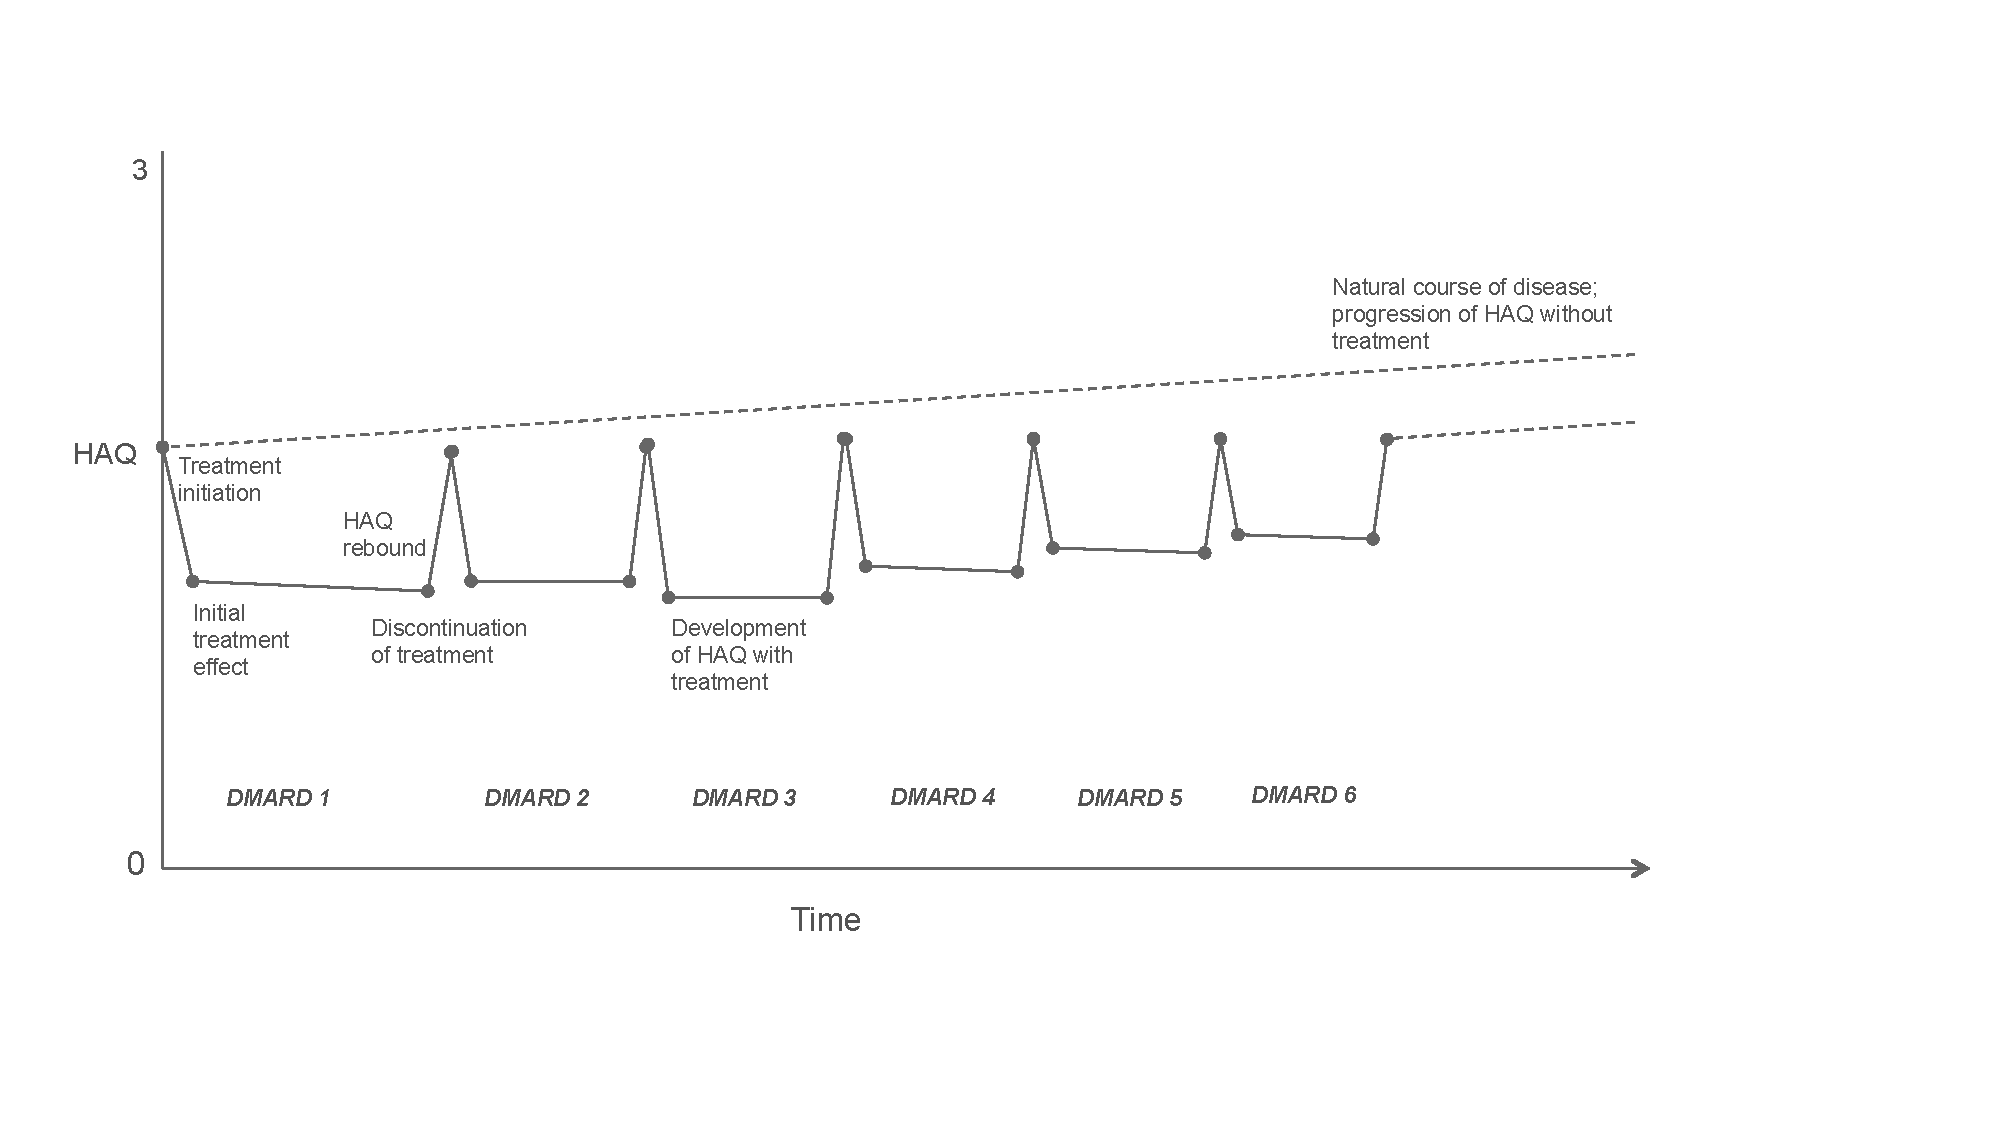
\includegraphics[max size={\textwidth}{\textheight}]{haq-structure.pdf}
\caption{Model structure regarding development of HAQ with sequential
biologic treatment}\label{fig:haq-structure}
\end{figure}

\subsection{Initial treatment phase}

During the initial treatment phase HAQ is modeled as a change from baseline.

\begin{itemize}
\item \textbf{H1}: Treatment $\rightarrow$ ACR $\rightarrow$ HAQ
\item \textbf{H2}: Treatment $\rightarrow$ ACR $\rightarrow$ EULAR $\rightarrow$ HAQ
\item \textbf{H3}: Treatment $\rightarrow$ HAQ
\end{itemize}

In \textbf{H1}, treatment influences HAQ through its effect on the American College of Rheumatology (ACR) response criteria, which is similar to the structure used in US based cost-effectiveness models \citep[e.g.][]{carlson2015economic, icer2017tim}. ACR 20/50/70 response is defined as at least a 20/50/70\% improvement. In the simulation, we convert these overlapping ACR categories to four mutually exclusive categories: no response (defined as less than 20\% improvement), ACR 20\% to <50\% improvement, ACR 50\% to <70\% improvement, and ACR 70\% improvement or greater. The rationale for using ACR response rather than HAQ directly is that the evidence base relating treatment to ACR response is larger than the evidence based relating treatment to HAQ. \textbf{H2} follows the National Institute for Health and Care Excellence (NICE) cost-effectiveness model \citep{stevenson2016adalimumab, stevenson2017cost} and models the effect of treatment on HAQ indirectly through its effect on ACR response and, in turn, the three categories of the European League Against Rheumatism (EULAR) response (no response, moderate response, or good response). Finally, since modeling the effect of treatment on HAQ through intermediary variables may mediate treatment response, in \textbf{H3}, treatment impacts HAQ directly.

Treatment switching during the initial treatment phase is modeled using 6 different pathways \textbf{S1-S6}.

\begin{itemize}
\item \textbf{S1:} Treatment $\rightarrow$ ACR $\rightarrow$ Switch
\item \textbf{S2:} Treatment $\rightarrow$ ACR $\rightarrow$ $\Delta$DAS28 $\rightarrow$ DAS28 $\rightarrow$ Switch 
\item \textbf{S3:} Treatment $\rightarrow$ ACR $\rightarrow$ $\Delta$SDAI $\rightarrow$ SDAI $\rightarrow$ Switch 
\item \textbf{S4:} Treatment $\rightarrow$ ACR $\rightarrow$ $\Delta$CDAI $\rightarrow$ CDAI $\rightarrow$ Switch 
\item \textbf{S5:} Treatment $\rightarrow$ $\Delta$DAS28 $\rightarrow$ DAS28 $\rightarrow$ Switch 
\item \textbf{S6:} Treatment $\rightarrow$ ACR $\rightarrow$ EULAR $\rightarrow$ Switch
\end{itemize}

\textbf{S1} follows a common approach where ACR non-responders discontinue treatment \citep[e.g.][]{carlson2015economic, icer2017tim}. One drawback of this approach is that it is not consistent with current treat-to-target guidelines in the United States \citep{singh20162015}. In \textbf{S2-S5}, treatment switching consequently depends on disease activity (remission, low, moderate, high) \citep{anderson2012rheumatoid}. In \textbf{S2-S4}, ACR response predicts the change in disease activity from baseline, which along with baseline disease activity, predicts absolute disease activity. Patients with moderate or high disease switch treatment while patients with low disease activity or in remission continue treatment. Disease activity is measured using either the Disease Activity Score with 28-joint counts (DAS28) \citep{prevoo1995modified}, Simplified Disease Activity Index (SDAI) \citep{smolen2003simplified, aletaha2005simplified}, or the Clinical Disease Activity Index (CDAI) \citep{aletaha2005acute}. 

\textbf{S5} is similar to \textbf{S2-S4}, but models the effect of treatment on changes in DAS28 directly, rather than indirectly through ACR response. We also aimed to model the direct effect of treatment on SDAI and CDAI, but sufficient clinical trial data are not available. Finally, since in the UK, the British Society for Rheumatology and the British Health Professionals in Rheumatology recommends using the EULAR response \citep{deighton2010bsr}, treatment switching in \textbf{S6} depends on EULAR response. In particular, following the NICE model, we assume that EULAR non-responders discontinue treatment while moderate and good responders continue treatment \citep{stevenson2016adalimumab}. The reasoning is that rules stipulated by NICE require a DAS28 improvement of more than 1.2 to continue treatment which is associated with moderate or good EULAR response. 

Not all pathways \textbf{S1-S6} can be used with each of \textbf{H1-H3}. If \textbf{H1} is used, then \textbf{S1-S5} are available, but \textbf{S6} is not because EULAR response is not simulated. In \textbf{H2}, \textbf{S1-S6} are all available while in \textbf{H3} only \textbf{S5} can be used since ACR response is not simulated. The 12 possible combinations are outlined in \autoref{tbl:initial-model-structure}.  

\begin{table}[!ht] 
\begin{center}
\begin{threeparttable}
\caption{Model structures for initial treatment phase} \label{tbl:initial-model-structure}
\begin{tabularx}{\textwidth}{@{\extracolsep{\fill}}lcccccc}
\hline
\multicolumn{1}{l}{} & \multicolumn{1}{c}{S1} & \multicolumn{1}{c}{S2} & \multicolumn{1}{c}{S3} & \multicolumn{1}{c}{S4} & \multicolumn{1}{c}{S5} & \multicolumn{1}{c}{S6}  \\
\hline
H1 & 1 & 2 & 3 & 4 & 5 & - \\
H2 & 6 & 7 & 8 & 9 & 10 & 11 \\
H3 & - & - & - & - & 12  & -\\
\hline
\end{tabularx}
\scriptsize
Notes: Rows denote the pathway used to relate treatment to HAQ and columns denote the pathway used to determine treatment switching. Each number denotes a unique combination of pathways (i.e., 1 corresponds to H1 and S1, and 8 corresponds to H2 and S3) and the ``-'' denotes a combination of pathways that is not possible. There are 12 possible model structures for the initial treatment phase. 
\end{threeparttable}
\end{center}
\end{table}

\subsection{Maintenance phase}
In the maintenance phase, the long-term progression of HAQ can be modeled in two ways. First, as is common in cost-effectiveness analyses (CEAs) of therapies for RA, HAQ is assumed to progress at a constant linear rate over time \citep[see][]{tosh2011sheffield, wailoo2008biologic}. However, since emerging evidence suggests that the rate of HAQ progression is non-linear and varies across patients \citep{gibson2016haq}, our second scenario simulates HAQ progression using a latent class growth model (LCGM) \citep{norton2014health} with 4 distinct HAQ trajectories and a rate of HAQ progression that decreases over time within each trajectory. Upon discontinuation of treatment, the HAQ score rebounds by a proportion of the improvement experienced at the end of the initial 6-month period with that treatment.

The duration of the maintenance phase (i.e., time to discontinuation of maintenance treatment) is simulated using parametric time-to-event distributions. When \textbf{S1} is used, time to treatment discontinuation is simulated using a single time-to-event curve because we have been unable to obtain curves stratified by ACR response categories. In contrast, when \textbf{S2-S5} are selected, the time-to-event curves are a function of disease activity level so patients with lower disease activity at the end of the initial treatment phase stay on treatment longer, on average. Likewise, when structure \textbf{S6} is used, the time-to-event distributions are stratified by EULAR response category and patients with good response at the end of the initial treatment phase tend to stay on treatment longer than patients with a moderate response. In each case, time to discontinuation can be simulated using one of 7 possible distributions (exponential, Weibull, Gompertz, gamma, log-logistic, lognormal, generalized gamma).

\subsection{Adverse events}
In line with \citet{stevenson2016adalimumab} the adverse events included in the model are limited to serious infections; we assume that only serious infections have a significant cost impact and increased risk over background rates to be meaningful to include \citep{ramiro2017safety}. During the initial treatment phase, a patient immediately stops treatment if a serious infection occurs; during the maintenance phase, time on treatment depends on the sampled time to treatment discontinuation and a patient experiences a serious infection if the individual's sampled time to the adverse event is shorter than the sampled time to treatment discontinuation. 

\subsection{Mortality}
Baseline HAQ scores (and changes in HAQ scores from baseline) are used to determine mortality relative to age/sex specific rates for the US general population (assumed to have a HAQ score of 0). Treatment, therefore, has an indirect effect on mortality through its effect on HAQ. 

\subsection{Utility}
Individual HAQ scores at a particular point in time were also used to simulate EuroQol five dimensions questionnaire (EQ-5D) utility scores (0-1 range), which, in turn, are used to simulate quality-adjusted life-years (QALYs). However, since a number of different methods have been used to convert HAQ into utility, our model contains two different possible mapping algorithms. Our preferred algorithm is the \citet{alava2013relationship} mixture model, which uses a much larger sample size than other statistical models and has been shown to have better predictive accuracy. Other algorithms are typically estimated using clinical trial data \citep[e.g.][]{carlson2015economic, stephens2015modelling} and consequently have limited generalizability. The second utility algorithm available within our model is based on a linear regression analysis of real-world data by \citet{wailoo2006modeling} that has been used in a few previous CEAs \citep[e.g.][]{wailoo2008biologic, icer2017tim}.

\subsection{Costs}
Annual hospitalization days and productivity losses are simulated as a function of HAQ. Health sector costs considered in the models are related to drug acquisition and administration, adverse events, general management of RA, and hospitalization. Non-health sector costs are limited to work-related productivity loss.

\subsection{Summary of simulation}
The flow diagram in \autoref{fig:flow-diagram} describes the flow of a single patient through the simulation. The simulation runs for a patient's entire lifespan beginning with treatment initiation and ending in death. The rectangles in the figure represent ``processes'' determining the effect of treatment on disease progression and the diamonds represent ``decisions'' that determine whether a patient will switch to a new treatment.

\begin{figure}
\centering
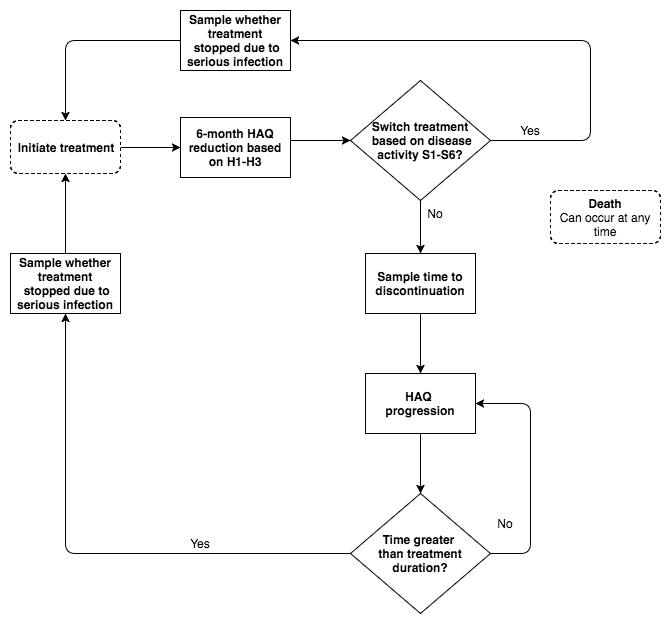
\includegraphics[max size={\textwidth}{\textheight}]{flow-diagram.png}
\caption{Flow diagram of the simulation for a single
patient}\label{fig:flow-diagram}
\begin{minipage}{\linewidth}
\footnotesize
Notes: Rectangles represent ``processes'' determining the effect of treatment on disease progression, Diamonds represent ``decisions'' that determine whether a patient will switch to a new treatment. Dotted lines denote start of a new treatment or the end of the simulation. 
\end{minipage}
\end{figure}

The influence diagram in \autoref{fig:influence-diagram} summarizes the assumed relationships among different variables in the model. Each arrow represents the direct effect of one parameter on another. Dashed lines represent relationships that depend on the structural assumptions used. \autoref{subfig:treatment-effects} focuses on the effect of treatment on disease progression and adverse events while \autoref{subfig:model-outcomes} looks at the relationships between the health and cost outcome variables. 

\begin{figure}
\centering
\begin{subfigure}{\textwidth}
\centering
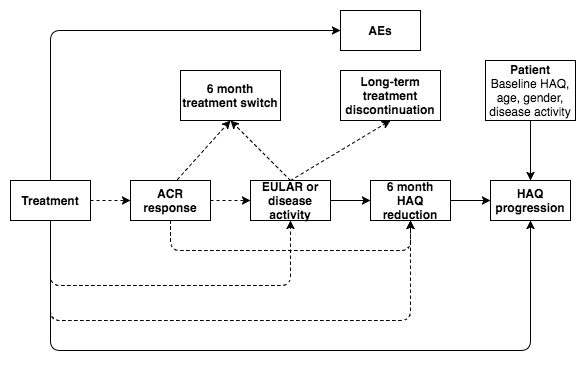
\includegraphics[width=\textwidth]{influence-diagram-a.png}
\caption{Treatment effects} \label{subfig:treatment-effects}
\end{subfigure}
\begin{subfigure}{\textwidth}
\centering
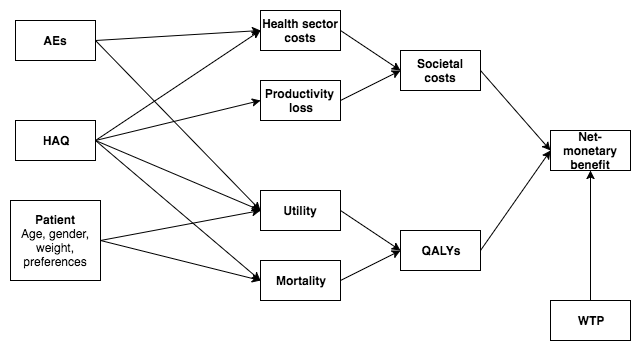
\includegraphics[width=.8\textwidth]{influence-diagram-b.png}
\caption{Long-term model outcomes} \label{subfig:model-outcomes}
\end{subfigure}
\caption{Influence diagram outlining structural relationships}\label{fig:influence-diagram}
\begin{minipage}{\linewidth}
\footnotesize
Notes: ACR: American College of Rheumatology; EULAR: European League Against Rheumatism; HAQ: Health Assessment Questionnaire: AEs: adverse events; QALYs: quality-adjusted life-years; WTP: willingness to pay. Disease activity refers to the Disease Activity Score with 28-joint counts (DAS28), the Simplified Disease Activity Index (SDAI), or the Clinical Disease Activity Index (CDAI).
\end{minipage}
\end{figure}

The model accounts for patient heterogeneity in two ways. First, baseline event rates vary across patients by both observable and unobservable factors. For example, long-term HAQ progression, mortality, and utility depend on patient specific variables including age, gender, and baseline disease level. Moreover, unobserved differences in long-term HAQ progression and utility across patients are modeled using mixture models. Second, relative treatment effects for ACR response, the change in HAQ at 6 months, and the change in DAS28 at 6 months, can be modeled as a function of explanatory variables in the \R{} package. 

\subsection{Model outcomes}\label{model-outcomes}
\subsubsection{Benefits, costs, and risks} \label{subsec:benefits-risks-costs}
The model simulates the health outcomes, costs, and risks associated with treatment. Depending on the model structure, model outcomes include the following:
\begin{itemize}
\item \textbf{Clinical outcomes during initial treatment phase}: ACR response, EULAR response, DAS28, SDAI, CDAI
\item \textbf{Long-term clinical outcomes}: HAQ, QALYs
\item \textbf{Adverse events}: number of serious infections
\item \textbf{Health care sector costs}: drug acquisition and administration costs, general management and monitoring costs, adverse event costs, hospitalization costs
\item \textbf{Non-health care sector costs}: productivity losses
\end{itemize}

\subsubsection{Outcomes for value assessment}
If CEA is used for value assessment, then the value of treatment is estimated using the NMB, as described in \autoref{sec:cea}. CEA from a societal perspective would include productivity losses while analyses from a health care sector perspective would not.

Any combination of simulated model outcomes can be used for MCDA. In IVI's web interfaces, the MCDA is currently based on the following criteria: (i) QALYs, (ii) total health care sector costs, (iii) productivity losses, (iv) number of serious infections, (v) route of administration (oral/injection/infusion) and (vi) time the medication has been on the market. We measure performance for each route of administration by calculating the percentage of total life-years that were spent using that particular route of administration. If a combination therapy is used during the treatment sequence, we allocate time equally among all routes of administration within the combination therapy (i.e., during a time period in which tofacitinib citrate is used with methotrexate, we allocate half of the time to oral admnistration and half to admnistration by injection). Performance on the time since the medication has been on the market criterion is a weighted average of time since FDA approval for each treatment in a treatment sequence, where weights are equal to the number of life-years spent using a particular treatment within the sequence. In the web interfaces users can input their own weights for each of the criteria, but it is important to note that we have not conducted the surveys required to elicit weights in a representative sample of patients. 

When analyzing value to healthy individuals---rather than sick patients---we use the framework described in \autoref{sec:braoder-value}. Following \citet{lakdawalla2015insurance} we calculate annual value for patients (e.g., benefits to an insurance enrollee during a plan year) by annualizing lifetime health gains (i.e., QALYs) and costs (see \autoref{app:insurance-value} for more details). To calculate the conventional value of a treatment to a healthy individual (i.e., $\pi( k \cdot dh - dp)$ from \autoref{eqn:insurance-value}), we estimate $dh$ using annualized incremental QALYs, $dp$ using annualized incremental costs, $k$ using willingness to pay thresholds, and $\pi$ as the probability of obtaining RA within the next year.  

\section{Source data and parameter estimation}\label{sec:data-parameters}

\subsection{Treatment effects at 6 months}\label{nma-parameters}
The effect of treatment on ACR response, DAS28, and HAQ at 6 months for tDMARD naive patients are estimated using Bayesian network meta-analyses (NMA) of published randomized controlled trials (RCTs). Primary outcomes were ACR response, change in DAS28 from baseline at 6 months, and the change in HAQ from baseline at 6 months. Results from the NMA are shown in \autoref{tbl:nma-acr-das28-haq}. Details of the systematic literature review and the statistical methodology are provided in the Appendix (\autoref{app:nma-analyses}).


\begin{sidewaystable}
\begin{center}
\begin{threeparttable}
\caption{Network meta-analysis estimates of ACR response, change in DAS28, and change in HAQ for tDMARD naive patients} \label{tbl:nma-acr-das28-haq}
\small
\begin{tabular}{lccccc}
\hline
\multicolumn{1}{c}{} & \multicolumn{3}{c}{ACR response} & \multicolumn{2}{c}{}\\
\cmidrule(lr){2-4} 
\multicolumn{1}{l}{} & \multicolumn{1}{c}{ACR20} & \multicolumn{1}{c}{ACR50} & \multicolumn{1}{c}{ACR70} & \multicolumn{1}{c}{$\Delta$DAS28} & \multicolumn{1}{c}{$\Delta$HAQ} \\
\hline
\ExpandableInput{tables/nma-acr-das28-haq.txt}
\hline
\end{tabular}
\scriptsize
Notes: ACR20/50/70 categories are the probability of at least a 20/50/70\% improvement. 95\% credible intervals are in parentheses. Estimates are based on 1,000 random draws of the NMA parameters. $\Delta$DAS28 and $\Delta$HAQ are changes in the DAS28 and HAQ score from their baseline scores respectively; negative numbers denote reductions in baseline values. cDMARDs = conventional disease-modifying antirheumatic drugs; MTX = methotrexate; ABT IV = abatacept intravenous; ABT SC = abatacept subcutaneous; ADA = adalimumab; ADA BWWD = adalimumab-bwwd (biosimilar Samsung Bioepis); ANA = anakinra; BCT = baricitinib; CZP = certolizumab pegol; ETN = etanercept; ETN SZZS = etanercept-szzs (biosimilar Sandoz); ETN YKRO = etanercept-ykro (biosimilar Samsung Bioepis); GOL = golimumab; HCQ = hydroxychloroquine sulfate; IFX = infliximab; IFX QBTX = infliximab-qbtx (biosimilar Pfizer); RTX = rituximab; SAR = sarilumab; SSZ = sulfazalazine; TCZ = tocilizumab; TOF = tofacitinib; UPA = upadacitinib;  ACR = American College of Rheumatology.
\end{threeparttable}
\end{center}
\end{sidewaystable}

Its important to note that treatment effects for each tDMARD were estimated relative to cDMARDs and then applied to the average response for patients using cDMARDs. A limitation of our current approach is that that the average response for patients using cDMARDs is estimated using data from the clinical trials include in the NMA, and may not reflect outcomes seen in routine practice. Future versions of the model could consider using real-world data instead of clinicial trial evidence to estimate this average response.

Given that there is limited evidence that treatment effects vary across patients in the published literature, treatment response at 6 months for a given treatment does not vary according to patient characteristics. Nonetheless, in our \R{} package, treatment effects for each simulated patient can be modeled as a function of any variables chosen by the user. Our approach to modeling treatment effect heterogeneity is described in \autoref{app:nma-analyses}. 

Treatment effects for tDMARD experienced patients are reduced by multiplying treatment effects for tDMARD naive patients by a constant $\gamma$. Based on evidence reported in \citet{carlson2015economic}, we assume that $\gamma$ is uniformly distributed and ranges between .75 and .92, implying that (rounding up) the average value of $\gamma$ is .84. In other words, reductions in DAS28 and HAQ scores for tDMARD experienced patients are, on average, 84\% of the reduction in DAS28 and HAQ scores for tDMARD naive patients, and an ACR response of 60/40/20 for tDMARD naive patients would, on average, be reduced to 50/33/16 for tDMARD experienced patients. 

In the simulation, treatment response depends on the line of therapy and whether a patient is tDMARD naive or tDMARD experienced at baseline. For tDMARD naive patients, first line treatment response is based on the NMA results for tDMARD naive patients while response for all other treatments in a treatment sequence is reduced using the constant $\gamma$. For tDMARD experienced patients, treatment response is reduced using $\gamma$ at each line of therapy including the first line. One limitation of this approach is that we are unable to model the relationship between line of therapy and $\gamma$; that is, treatment response for a patient who has failed at least one biologic is assumed to be reduced by, on average, .84, regardless of line of therapy. 

\subsection{Treatment switching at 6 months}
The data required to determine treatment switching at 6 months depends on the selected model structure. If \textbf{S1} is selected, then treatment switching depends on the simulated ACR response; likewise, if \textbf{S5} is selected, then treatment switching depends on the simulated level of DAS28 at 6 months. When \textbf{S2-S4} are used, treatment switching is determined by the relationship between ACR response and the change in disease activity, and in \textbf{S6}, switching is based on the relationship between ACR response and EULAR response. Details of the mapping between ACR response and change in disease activity and between ACR response and EULAR response are provided below.  

\subsubsection{ACR response and change in disease activity}
There are currently no established mappings between mutually exclusive ACR response categories and DAS28, SDAI, or CDAI \citep{madan2015consensus}. However, \citet{aletaha2005simplified} provides evidence on the relationship between overlapping ACR response categories (ACR 20/50/70) and mean changes in each of the three disease activity measures. Results are reported for three cohorts---the Leflunomide datasets, the inception cohort, and the routine cohort---with 1,839, 91, and 279 patients, respectively. We transformed mean changes by overlapping ACR response categories to mean changes by mutually exclusive ACR response categories by using the number of patients in each mutually exclusive ACR response category as described in \autoref{app-acr-da}. \citet{smolen2003simplified} provided the number of patients in each ACR response category in the Leflunomide dataset and \citet{aletaha2005acute} provided the number of patients in the inception cohort. Mean changes in disease activity in each mutually exclusive ACR response category are shown in \autoref{tbl:acr2da}. However, note that the referenced publications did not report mean outcomes, so we were unable to generate standard errors for the estimates. We consequently assume allow the estimates to vary by 20\% in either direction.  


\begin{table}[!ht]
\begin{center}
\begin{threeparttable}
\caption{Relationship between ACR response and change in disease activity measures} \label{tbl:acr2da}
\begin{tabularx}{\textwidth}{@{\extracolsep{\fill}}lcccc}
\hline
\multicolumn{1}{l}{ACR response} &  \multicolumn{3}{c}{Mean change at 6 months}\\
\cmidrule{2-5}
\multicolumn{1}{l}{} & \multicolumn{1}{c}{Leflunomide dataset} & \multicolumn{3}{c}{Inception cohort}\\
\cmidrule(lr){2-2}  \cmidrule(lr){3-5}
\multicolumn{1}{c}{} & \multicolumn{1}{c}{SDAI} & \multicolumn{1}{c}{SDAI} &\multicolumn{1}{c}{CDAI} & \multicolumn{1}{c}{DAS28} \\
\hline
\ExpandableInput{tables/acr2da.txt}
\hline
\end{tabularx}
\scriptsize
Sources: \citet{aletaha2005simplified}, \citet{smolen2003simplified}, and  \citet{aletaha2005acute} 
\end{threeparttable}
\end{center}
\end{table}

We did not include estimates from the routine cohort for two reasons. First, we were unable to find information on the number of patients in each ACR response category. Second, patients in the routine cohort had considerably lower disease activity levels \citep{aletaha2005simplified, aletaha2005acute} and our default population (see \autoref{sec:populations}) consists of patients with high disease activity at baseline. Mean DAS28 in the inception cohort and routine cohort were 5.62 and 4.09, respectively, while the mean DAS 28 ranged from 6.3 to 7 across the clinical trials making up the Leflunomide dataset.

\subsubsection{ACR response and change in EULAR response}
ACR responses were translated into EULAR response probabilities based on evidence of their relationship reported in \citet{stevenson2016adalimumab} and obtained from the US Veterans Affairs Rheumatoid Arthritis (VARA) registry (\autoref{tbl:acr2eular}).



\begin{table}[!ht]
\begin{center}
\begin{threeparttable}
\caption{Relationship between ACR response and EULAR response} \label{tbl:acr2eular}
\begin{tabularx}{\textwidth}{@{\extracolsep{\fill}}lcccc}
\hline
\multicolumn{1}{l}{} & \multicolumn{3}{c}{EULAR response} \\
\cmidrule{2-4} 
\multicolumn{1}{c}{ACR response} & \multicolumn{1}{c}{None} & \multicolumn{1}{c}{Moderate} & \multicolumn{1}{c}{Good} \\
\hline
\ExpandableInput{tables/acr2eular.txt}
\hline
\end{tabularx}
\scriptsize
Notes: Obtained from the US Veterans Affairs Rheumatoid Arthritis (VARA) registry by \citet{stevenson2016adalimumab}. The VARA registry is a multicentre, US database of veterans age 19 and older. Each cell represents the number of patients in the database in a given category. 
\end{threeparttable}
\end{center}
\end{table}

\subsection{Change in HAQ at 6 months}
In model structures including \textbf{H1}, the impact of treatment on changes in HAQ at 6 months is modeled by first estimating the effect of treatment on ACR response and then mapping ACR response to a change in HAQ. As in \citet{icer2017tim}, ACR responses from the NMA were translated into HAQ scores based on evidence from the adalimumab monotherapy for treatment of rheumatoid arthritis (ADACTA) trial reported in \citet{carlson2015economic} (\autoref{tbl:acr2haq}).


\begin{table}[!ht]
\begin{center}
\begin{threeparttable}
\caption{Relationship between ACR response and change in HAQ at 6 months} \label{tbl:acr2haq}
\begin{tabularx}{\textwidth}{@{\extracolsep{\fill}}lcc}
\hline
\multicolumn{1}{l}{} & \multicolumn{2}{c}{HAQ change} \\
\cmidrule{2-3} 
\multicolumn{1}{c}{ACR response} & \multicolumn{1}{c}{Mean} & \multicolumn{1}{c}{Standard error} \\
\hline
\ExpandableInput{tables/acr2haq.txt}
\hline
\end{tabularx}
\scriptsize
Source: \citet{carlson2015economic}
\end{threeparttable}
\end{center}
\end{table}


The relationship between EULAR response and HAQ is based on analyses conducted by \citet{stevenson2016adalimumab} using the BSRBR database. Their analysis is based on predictions from a mixture model with covariates set to sample means. Moderate and good EULAR responses are associated with -0.317 (SE = 0.048) and -0.672 (SE = 0.112) changes in HAQ scores respectively (\autoref{tbl:eular2haq}). 

\begin{table}[!ht]
\begin{center}
\begin{threeparttable}
\caption{Relationship between EULAR response and change in HAQ at 6 months} \label{tbl:eular2haq}
\begin{tabularx}{\textwidth}{@{\extracolsep{\fill}}lcc}
\hline
\multicolumn{1}{c}{EULAR response} & \multicolumn{1}{c}{Mean} & \multicolumn{1}{c}{Standard error} \\
\hline
\ExpandableInput{tables/eular2haq.txt}
\hline
\end{tabularx}
\scriptsize
Notes: Based on an analysis of the BSRBR database by \citet{stevenson2016adalimumab}.
\end{threeparttable}
\end{center}
\end{table}

\autoref{tbl:sim-haq-change} compares the impact of treatment on HAQ when using \textbf{H1-H3}. Results were estimated by simulating $1,000$ patients for 6 months and randomly sampling $1,000$ parameter sets. For each randomly sampled parameter set, we calculated the average decrease in HAQ at 6 months across the $1,000$ patients. Estimates reported in the table are the mean and 95\% credible interval of the mean decrease in HAQ at 6 months. To maintain consistency across \textbf{H1-H3}, we did not allow HAQ scores for patients who might have otherwise switched treatments accoring to \textbf{S1-S6} to rebound back to their baseline levels (i.e., levels at the start of the simulation) at the end of the 6 month period.   



\begin{table}[!ht]
\begin{center}
\begin{threeparttable}
\caption{Simulated mean change in HAQ at 6 months under different model structures} \label{tbl:sim-haq-change}
\begin{tabularx}{\textwidth}{@{\extracolsep{\fill}}lccc}
\hline
\multicolumn{1}{l}{} & \multicolumn{1}{c}{\textbf{H1}} & \multicolumn{1}{c}{\textbf{H2}} & \multicolumn{1}{c}{\textbf{H3}} \\
\hline
\ExpandableInput{tables/sim-dhaq-6months.txt}
\hline
\end{tabularx}
\scriptsize
Notes: \textbf{H1}, \textbf{H2}, and \textbf{H3} are the Treatment $\rightarrow$ ACR $\rightarrow$ HAQ, Treatment $\rightarrow$ ACR $\rightarrow$ EULAR $\rightarrow$ HAQ, and Treatment $\rightarrow$ HAQ pathways respectively. 95\% credible intervals are in parentheses. Estimates are based on 6-month simulations of 1,000 patients and 1,000 parameters sets for each therapy. $\Delta$HAQ denotes a change in the HAQ score at 6 months from baseline; a negative value indicates a reduction in the HAQ score. Mean $\Delta$HAQ is calculated for each parameter set by averaging across the 1,000 patients. cDMARDs = conventional disease-modifying antirheumatic drugs; MTX = methotrexate; ABT IV = abatacept intravenous; ABT SC = abatacept subcutaneous; ADA = adalimumab; ADA BWWD = adalimumab-bwwd (biosimilar Samsung Bioepis); ANA = anakinra; BCT = baricitinib; CZP = certolizumab pegol; ETN = etanercept; ETN SZZS = etanercept-szzs (biosimilar Sandoz); ETN YKRO = etanercept-ykro (biosimilar Samsung Bioepis); GOL = golimumab; HCQ = hydroxychloroquine sulfate; IFX = infliximab; IFX QBTX = infliximab-qbtx (biosimilar Pfizer); RTX = rituximab; SAR = sarilumab; SSZ = sulfazalazine; TCZ = tocilizumab; TOF = tofacitinib; UPA = upadacitinib;  ACR = American College of Rheumatology. 
\end{threeparttable}
\end{center}
\end{table}

Estimates for \textbf{H1} and \textbf{H3} are generally similar but treatment response is considerably smaller when using \textbf{H2}. This suggests that the additional mapping between ACR response and EULAR response attenuates treatment response. Given these varying estimates of the change in HAQ during the initial treatment phase and the impact of HAQ on other important outcomes within the model including utility and health care costs, the choice of \textbf{H1-H3} (and in particular \textbf{H2} vs. \textbf{H1/H3}) appears to have important consequences for value assessment.  

\subsection{HAQ progression in the absence of tDMARD treatment}\label{haq-progression-in-the-absence-of-tDMARD-treatment}

The natural course of HAQ progression in the absence of tDMARDs develops over time according to an estimated natural course for patients remaining on cDMARDs or following discontinuation of the last tDMARD of the sequence (i.e., on NBT). The natural course of HAQ can either be assumed to change at a constant linear rate or be modeled using a LCGM that accounts for non-linear progression and heterogeneity across patients. 

\subsubsection{Constant linear rate of progression} \label{sec:haq-linear-rate}
The rate of progression in the linear case is based on the observational study by \citet{wolfe2010loss}. They assessed the development of HAQ over time at six month intervals for up to 11 years among 3,829 RA patients who switched from non-biologic treatment to biologic treatment and participated in the National Data Bank for Rheumatic Diseases (NDB) longitudinal study of RA outcomes. The annual HAQ progression rate prior to biologic therapy was 0.031 (95\% confidence interval (95\%CI): 0.026 to 0.036) and is assumed to reflect the course of progression of HAQ in the absence of tDMARDs.

Based on the same data, \citet{michaud2011treatment} reported overall and age-specific specific HAQ progression rates. The differences between the overall and age specific rates are as follows: \textless{}40: -0.020 (95\%CI: -0.0223 to -0.0177); 40-64: -0.008 (95\%CI: -0.0101 to -0.0059); \(\geq\) 65 0.017 (95\%CI: 0.0136 to 0.0204). These estimates are applied to the overall progression rate of 0.031 to obtain age specific HAQ progression rates (see \autoref{app:age-linear-haq}).


\begin{table}[!ht]
\begin{center}
\begin{threeparttable}
\caption{Annual linear progression of HAQ in the absence of tDMARDs beyond 6 months} \label{tbl:haq-lprog}
\footnotesize
\begin{tabularx}{\textwidth}{@{\extracolsep{\fill}}lrrrl}
\hline
\multicolumn{2}{l}{} & \multicolumn{2}{c}{95\% CI} & \multicolumn{1}{l}{} \\
\cmidrule{3-4} 
\multicolumn{1}{l}{} & \multicolumn{1}{r}{Estimate} & \multicolumn{1}{r}{Lower} & \multicolumn{1}{r}{Upper} & \multicolumn{1}{l}{Reference} \\
\hline
Overall progression rate \\
\ExpandableInput{tables/haq-lprog-cdmards.txt}
Change in overall progression rate by age \\
\ExpandableInput{tables/haq-lprog-diff-byage.txt}
\hline
\end{tabularx}
\scriptsize
Notes: 95\% confidence intervals are calculated using a normal distribution. Confidence intervals for changes in HAQ progression rates by age assume no covariance between the overall progression rate and the age-specific rates reported by \citet{michaud2011treatment}.
\end{threeparttable}
\end{center}
\end{table}

\subsubsection{Latent class growth model} \label{sec:haq-lcgm}
We also model the rate of HAQ progression in the absence of tDMARDs using a mixture model approach that has increasingly been used to model HAQ progression over time \citep{stevenson2016adalimumab, norton2013trajectories, norton2014health}. These models suggest that different subgroups have distinct HAQ trajectories and that the rate of worsening of HAQ progression decreases over time. We use the LCGM estimated by \citet{norton2014health} and since we aim to model trajectories for cDMARDs and NBTs we chose the specification based on data from the Early Rheumatoid Arthritis Cohort Study (ERAS) cohort, which has a high percentage of patients receiving methotrexate and a very small percentage receiving biologics. Complete details of the LCGM are provided in \autoref{app:lcgm-haq}. 


The \citet{norton2014health} LCGM determined that there are four classes of patients and thus four distinct HAQ trajectories. The probability of class membership depends on 7 variables: age, gender, DAS28, disease duration, rheumatoid factor, the ACR 1987 criteria for RA, and a measure of socioeconomic status. Age, gender, and the DAS28 are relevant to the way the population is defined within our model (see \autoref{sec:populations}) and are therefore important determinants of the HAQ trajectory. Other variables (disease duration, rheumatoid factor, ACR criteria, and socioeconomic status) are not defined within our population. We consequently set disease duration (8.2 months), rheumatoid factor (0.73), and the socioeconomic status variable (0.49) equal to their mean values with the ERAS cohort. The ACR criteria was set to 1. 

HAQ trajectories (in levels) by class are shown \autoref{fig:lcgm-haq-prog}. The dotted lines plot observed mean values. There are clear distinguishable classes as both the level of the HAQ score and its slope vary between groups. \citet{norton2014health} refer to the groups as ``low'', ``moderate'', ``high'', and ``severe'' groups, in order from the lowest to highest HAQ scores. The observed trends for the low, medium, and high groups follow a J-shaped pattern with a sharp drop following treatment initiation and an upward slope thereafter, while the severe group experiences persistently high HAQ scores. Since our model separates the initial treatment phase from the maintenance phase, we are only concerned with HAQ progression following the initial drop. As in \citet{stevenson2016adalimumab}, we consequently only predict values from year 2 onward. The fitted values are the solid upward sloping lines in the plot.  
\begin{figure}[H]
\centering
\includegraphics[max size={.8\textwidth}{.8\textheight}]{../../data-raw/figs/haq-lcgm-obsexp.pdf}
\caption{Observed and predicted HAQ trajectories in the ERAS dataset from the latent class growth model}\label{fig:lcgm-haq-prog}
\begin{minipage}{\linewidth}
\footnotesize
Notes: The first three data points corresponds to years 0, 0.5, and 1, respectively; all other data points are spaced 1 year apart.
\end{minipage}
\end{figure}


An important question for modeling disease progression in RA is how the rate of progression within each class in the LCGM compares to a constant linear trajectory. We examine this question in \autoref{fig:lcgm-vs-linear}, which compares yearly rates of changes in HAQ using the LCGM and with constant annual rates of change (0.031 per year) based on the \citet{wolfe2010loss} analysis. The LCGM was simulated over 30 years and differences between year $t$ and year $t-1$ were used to assess changes in HAQ score from one year to the next.  

In the moderate, high, and severe groups the rate of HAQ progression is higher initially in the LCGM than in the \citet{wolfe2010loss} analysis; however, the LCGM modeled rate of HAQ progression declines over time and eventually begins to approach zero. In the low group, HAQ increases at a rate less than 0.031 per year and the rate of increase declines over time. 

\begin{figure}[H]
\centering
\includegraphics[max size={.7\textwidth}{.7\textheight}]{figs/haq-lcgm-vs-linear.png}
\caption{A comparison of predicted yearly changes in HAQ between a latent class growth model and constant linear progression from year 2 onwards}\label{fig:lcgm-vs-linear}
\end{figure}

\subsection{HAQ trajectory with tDMARD maintenance treatment}
Based on the NDB longitudinal study, \citet{wolfe2010loss} estimated the overall annual HAQ progression rate among RA patients who had switched to biologic treatment at -0.001 (95CI: -0.004 to 0.002). In a separate analysis, also based on NDB data, \citet{michaud2011treatment} reported annual HAQ progression rates by treatment adjusted for baseline HAQ score, age, sex, education, smoking, BMI, comorbidity, and RA onset. The average HAQ rate among patients on a biologic was -0.001 as well, which instills confidence that the reported HAQ progression rates for different biologics as reported by \citet{michaud2011treatment} can be directly compared with the overall annual HAQ progression rate of 0.031 reported by \citet{wolfe2010loss}. Accordingly, biologic specific HAQ progression rates by \citet{michaud2011treatment} are used in the model. For tDMARD treatments evaluated in the model for which no HAQ progression rate was reported by \citet{michaud2011treatment}, the overall biologic rate of -0.001 is used. 

\subsection{Duration of maintenance treatment}\label{duration-of-maintenance-treatment}
Time to treatment discontinuation in the maintenance phase depends on the pathway (\textbf{S1-S6}) used to model treatment switching. If \textbf{S1} is selected, a single treatment discontinuation curve based on an analysis from the CORRONA database is used for all patients. In \textbf{S2-S5}, time to treatment discontinuation is stratified by the level of disease activity, and in \textbf{S6} treatment duration depends on EULAR response.  

\subsubsection{Treatment duration in the US}\label{sec:ttd-overall}
We based our estimates of treatment duration during the maintenance phase for patients in the US with analyses of the CORRONA database \citep{strand2013op0064}. The analysis sample consisted of 6,209 patients age 18 or older treated between 2002 and 2011 receiving either TNF inhibitors or other bDMARDs. The mean age was 57.6 years, 43\% of patients were biologic naive, the mean CDAI was 16, and just over 26\% of patients had high disease activity (CDAI $\geq$ 22). 

7 parametric survival models (exponential, Weibull, Gompertz, gamma, log-logistic, lognormal, and generalized gamma) were estimated on individual patient data reconstructed from a Kaplan-Meier curve from the CORRONA analysis using the algorithm developed in \citet{guyot2012enhanced}. We compared fit using the Akaike Information Criteria (AIC) and Bayesian Information Criteria (BIC). The generalized gamma had the lowest AIC and BIC, so we consider it to be the preferred model. A plot of of the generalized gamma distribution against the Kaplan-Meier curve is shown in \autoref{fig:corrona-gg}. As can be seen in the plot, the shape of the survival curve estimated using a generalized gamma distribution tracks the Kaplan-Meier curve closely.  


\begin{table}[!ht]
\begin{center}
\begin{threeparttable}
\caption{AIC and BIC for parametric models of treatment duration from the CORRONA database} \label{tbl:ic-ttd-corrona}
\begin{tabularx}{\textwidth}{@{\extracolsep{\fill}}lcccc}
\hline
\multicolumn{1}{l}{Distribution} & \multicolumn{1}{c}{AIC} & \multicolumn{1}{c}{BIC}  \\
\hline
\ExpandableInput{tables/ttd-corrona-ipdsurv-ic.txt}
\hline
\end{tabularx}
\end{threeparttable}
\end{center}
\end{table}

\begin{figure}[h]
\centering
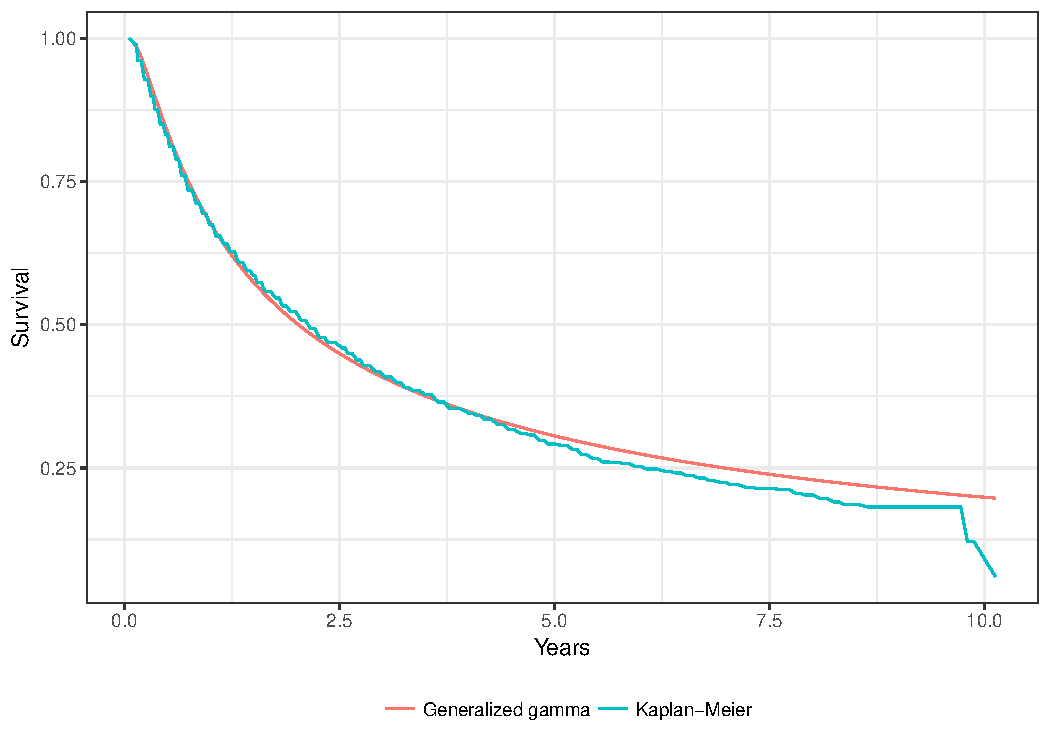
\includegraphics[max size={.7\textwidth}{.7\textheight}]{../../data-raw/figs/ttd-corrona-ipdsurv-gengamma.pdf}
\caption{Generalized gamma and Kaplan-Meier time to treatment discontinuation curves using reconstructed individual patient data from the CORRONA database}\label{fig:corrona-gg}
\end{figure}

We considered estimating separate time to discontinuation curves for each treatment, but did not for a number of the reasons cited in \citet{stevenson2016adalimumab}. The majority of the literature focuses on anti-TNFs (e.g., infliximab, etanercept, and adalimumab) \citep[e.g.][]{gomez2006switching, yazici2009changing, pan2009comparison}, which makes it difficult to estimate discontinuation curves for the other treatments. Furthermore, studies comparing rates of discontinuation across treatments tend to be observational because clinical trials are of short duration and do not reflect real-world patient populations. However, although observational studies provide accurate predictions on time to discontinuation, it is difficult to avoid bias from confounding when estimating differences across treatments because patients are not randomized into treatment and control groups \citep{souto2015rate} .   

We also lack data on treatment duration for patients on cDMARDs. Following \citet{stevenson2016adalimumab}, we assume that, conditional on continuing treatment at 6 months, treatment duration for tDMARDs is applicable to treatment duration for cDMARDs. This is, in turn, based on the assumption that cDMARDs are not likely to be more toxic than biologics used in combination with cDMARDs.

\subsubsection{Treatment duration by disease activity level}\label{ttd-da}
When \textbf{S2-S5} are selected, treatment duration is stratified by the level of disease activity. Since patients in the CORRONA database tended to have moderate disease activity (mean CDAI = 16), we use the CORRONA survival curve to model treatment duration for patients with moderate disease activity. We adjust this curve for patients in remission or low disease activity using the odds ratios reported in \citet{zhang2011thresholds}, which imply that patients in remission or with low disease activity have .52 times the odds of stopping treatment as patients with moderate disease activity. In particular, we adjust the probability of treatment failure at each point in time using the methodology described in \autoref{app:odds-ratio-prob}. As with the analysis described in \autoref{sec:ttd-overall}, we then fit 7 parametric survival models to individual patient data reconstructed from the adjusted survival curve using the \citet{guyot2012enhanced} algorithm. Generalized gamma time to treatment discontinuation curves stratified by disease activity level are shown in \autoref{fig:ttd-gg-da}. Survival curves for patients with severe disease activity are not displayed because patients with severe disease activity are assumed to switch treatments after the first 6 months of treatment.

\begin{figure}[H]
\centering
\includegraphics[max size={.6\textwidth}{.6\textheight}]{../../data-raw/figs/ttd-corrona-ipdsurv-gengamma-by-da.pdf}
\caption{Generalized gamma time to treatment discontinuation curves by disease activity level}\label{fig:ttd-gg-da}
\begin{minipage}{\linewidth}
\footnotesize
Notes: The shaded region denotes the simulation based 95\% confidence interval \citep{mandel2013simulation}.
\end{minipage}
\end{figure}

\subsubsection{Treatment duration by EULAR response} \label{ttd-eular}
In \textbf{S6}, we stratify time to treatment discontinuation by EULAR response based on analyses of the British Society for Rheumatology Biologics Registers (BSRBR) database \citep{stevenson2016adalimumab}. We again fit 7 parametric survival models using reconstructed individual patient data. The survival curves reported in \citet{stevenson2016adalimumab} were used to create the patient data. The AIC and BIC of each model by EULAR response category are shown in \autoref{tbl:ic-dur-eular}.


\begin{table}[!ht]
\begin{center}
\begin{threeparttable}
\caption{AIC and BIC for parametric models of treatment duration by EULAR response} \label{tbl:ic-dur-eular}
\begin{tabularx}{\textwidth}{@{\extracolsep{\fill}}lcccc}
\hline
\multicolumn{1}{l}{} & \multicolumn{2}{c}{Moderate EULAR response} & \multicolumn{2}{c}{Good EULAR response} \\
\cmidrule{2-3} \cmidrule{4-5}
\multicolumn{1}{l}{Distribution} & \multicolumn{1}{c}{AIC} & \multicolumn{1}{c}{BIC} & \multicolumn{1}{c}{AIC}  & \multicolumn{1}{c}{BIC}   \\
\hline
\ExpandableInput{tables/ttd-bsrbr-ipdsurv-eular-ic.txt}
\hline
\end{tabularx}
\end{threeparttable}
\end{center}
\end{table}

One concern is that the BSRBR is representative of the UK but not the US. As a result, we also estimate ``adjusted'' survival models appropriate for US based analyses. The adjustment is made in six steps using the analyses from the CORRONA database described in \autoref{sec:ttd-overall}. 

\begin{enumerate}
\def\labelenumi{\arabic{enumi}.}
\item Calculate a hazard function based on a survival curve from an analysis
  of the CORRONA database. In particular, reconstruct individual patient
  data from the survival curve \citep{guyot2012enhanced} and fit a
  spline-based survival model. Then use the spline-based model to
  estimate the hazard function $h(t)_{corrona}$.
\item Calculate a hazard function based on the BSRBR. To do so, first
  calculate hazard functions for both moderate and good EULAR responders
  using the same method described in step 1. Then calculate an overall
  hazard function with the proportion of moderate and good responders in
  the BSRBR analysis. Given that the number of moderate responders is
  \(5,492\) and the number of good responders is $2,417$ the overall
  hazard function is $h(t)_{bsrbr} = \frac{5,492}{7,909}h(t)_{bsrbr, moderate} + \frac{2,417}{7,909}h(t)_{bbsrbr, good}$.
\item At each point in time, calculate the ratio of the CORRONA and BSRBR
  hazard functions: $HR(t) = h(t)_{corrona}/h(t)_{bbsrbr}$.
\item Apply the hazard ratio in step 3 to the BSRBR hazard functions for
  each EULAR response category. That is $h(t)_{bsrbr, moderate, adj} = h(t)_{bsrbr, moderate} \cdot HR(t)$ and $h(t)_{bsrbr, good, adj} = h(t)_{bsrbr, good} \cdot HR(t)$.
\item Generate survival curves using the hazard functions from step 4.
  Specifically, given a general hazard function $h(t)$, calculate the
  cumulative hazard function, $H(t) = \int_{z = 0}^{t} h(z)dz$,
  convert this to a survival function using $S(t) = exp(-H(t))$, and
  reconstruct individual patient data using the survival curve.
\item Fit parametric survival models to the individual patient data
  generated in step 5.
\end{enumerate}

Both adjusted and unadjusted survival curves by EULAR response fit using a generalized gamma distribution are shown in \autoref{fig:bsrbr-gg}. AIC and BIC for the parametric models fit in step 6 to the adjusted individual patient data are shown in \autoref{tbl:ic-dur-adj-eular}.

\begin{figure}[h]
\centering
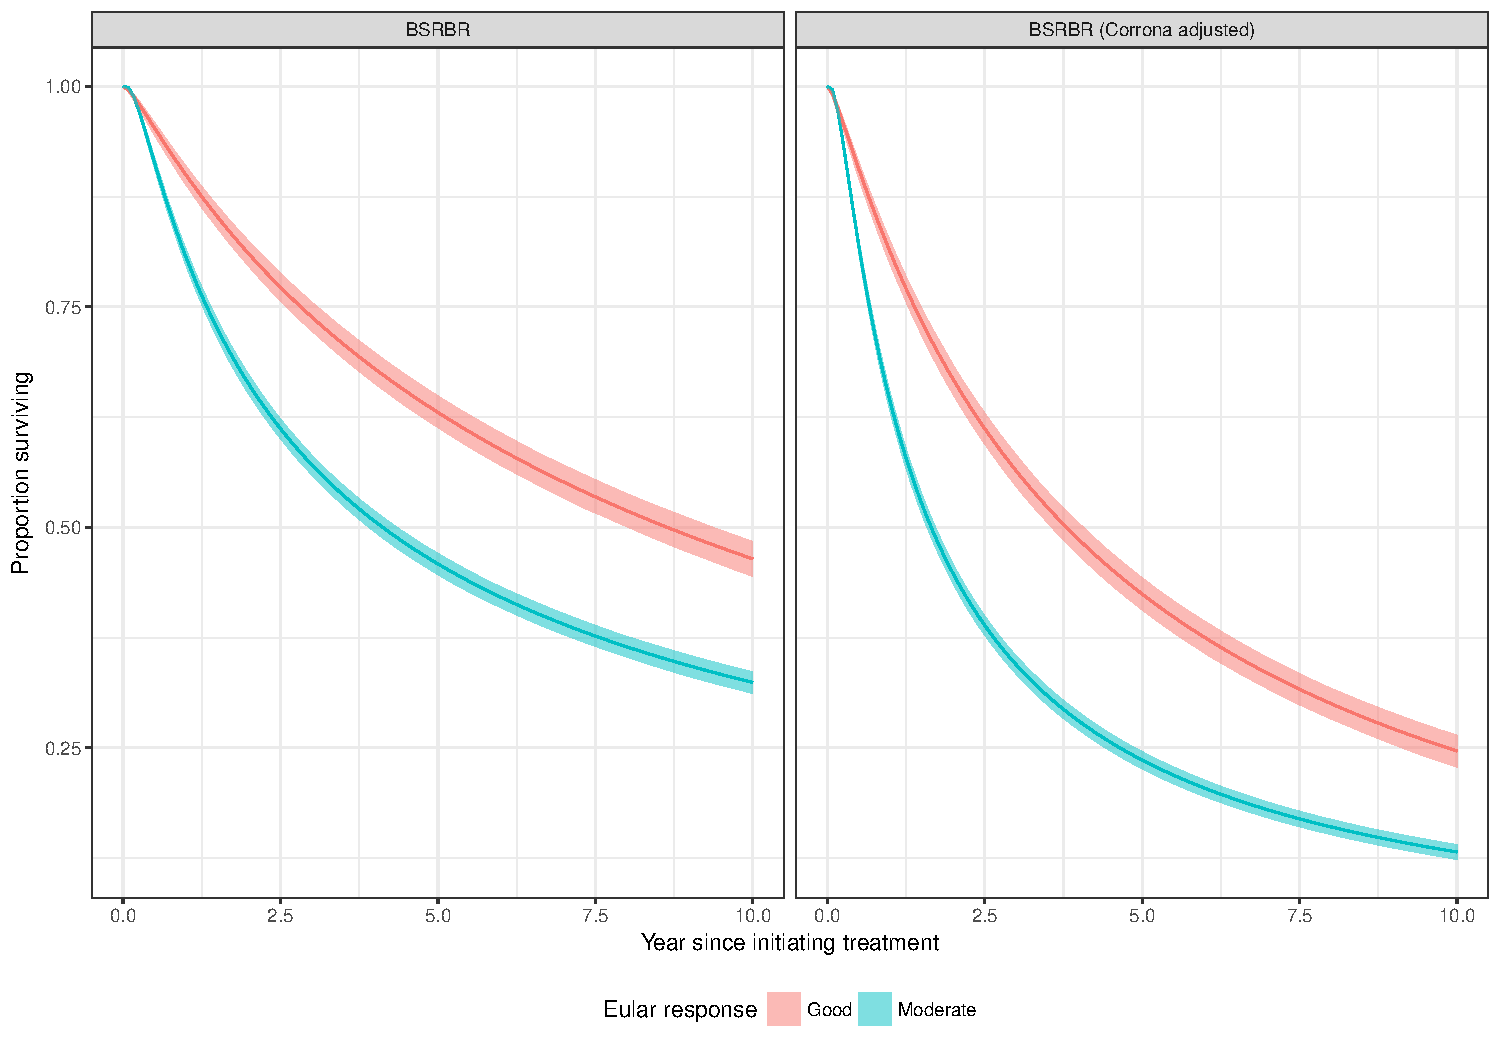
\includegraphics[max size={.7\textwidth}{.7\textheight}]{../../data-raw/figs/ttd-bsrbr-ipdsurv-comp-gengamma-by-eular.pdf}
\caption{Generalized gamma survival curve of treatment duration using reconstructed individual patient data based on analyses from Stevenson et al. (2016) by EULAR response category}\label{fig:bsrbr-gg}
\begin{minipage}{\linewidth}
\footnotesize
Notes: The shaded region denotes the simulation based 95\% confidence interval \citep{mandel2013simulation}.
\end{minipage}
\end{figure}



\begin{table}[!ht]
\begin{center}
\begin{threeparttable}
\caption{AIC and BIC for CORRONA adjusted parametric models of treatment duration by EULAR response} \label{tbl:ic-dur-adj-eular}
\begin{tabularx}{\textwidth}{@{\extracolsep{\fill}}lcccc}
\hline
\multicolumn{1}{l}{} & \multicolumn{2}{c}{Moderate EULAR response} & \multicolumn{2}{c}{Good EULAR response} \\
\cmidrule{2-3} \cmidrule{4-5}
\multicolumn{1}{l}{Distribution} & \multicolumn{1}{c}{AIC} & \multicolumn{1}{c}{BIC} & \multicolumn{1}{c}{AIC}  & \multicolumn{1}{c}{BIC}   \\
\hline
\ExpandableInput{tables/ttd-bsrbr-ipdsurv-eular-adjusted-ic.txt}
\hline
\end{tabularx}
\end{threeparttable}
\end{center}
\end{table}

\FloatBarrier


\subsection{Rebound post treatment}
Since no data exists on the size of the HAQ rebound post treatment, we vary its size as a proportion of the initial 6-month HAQ decline. 1 is used as an upper bound, which implies that the HAQ rebound is equal to the improvement experienced at the end of the initial 6-month period with that treatment. 0.7 is currently used as a lower bound.

\subsection{Serious infections}
Based on the NMA by \citet{singh2011adverse} and in accordance with \citet{stevenson2016adalimumab}, we assume a rate of 0.035 (95\% CI: 0.027 to 0.046) infections per person-year with all tDMARDs and a rate of 0.026 (no CI reported) infections per person-year with cDMARDs. The rate of infection is assumed to be equal across tDMARDs because the published results for specific tDMARDs are estimated with very little precision. The standard error on the infection rate for tDMARDs is assumed to be the same as the standard error for cDMARDs since no standard error was reported for tDMARDs in \citet{singh2011adverse}.


A patient in the IPS has a serious infection if the simulated time to serious infection occurs before the simulated time of treatment discontinuation. \autoref{tbl:si-prob} shows the probability of this occurring when treatment duration is modeled using a generalized gamma distribution. The probability of a serious infection is relatively rare as only 3.82\% of patients using cDMARDs and 8.55\% of patients using tDMARDs have serious infections. However, differences between cDMARDs and tDMARDs are not insignificant as the probability of a serious infection is almost 5 percentage points higher with tDMARDs than with cDMARDs.

\begin{table}[!ht]
\begin{center}
\begin{threeparttable}
\caption{Probability of serious infection} \label{tbl:si-prob}
\begin{tabularx}{\textwidth}{@{\extracolsep{\fill}}lrrr}
\hline
\multicolumn{1}{l}{} & \multicolumn{3}{c}{Probability} \\
\cmidrule{2-4} 
\multicolumn{2}{l}{} & \multicolumn{2}{c}{95\% CI} \\
\cmidrule{3-4} 
\multicolumn{1}{c}{} & \multicolumn{1}{c}{Mean} & \multicolumn{1}{c}{Lower} & \multicolumn{1}{c}{Upper} \\
\hline
\ExpandableInput{tables/si-prop-gengamma.txt}
\hline
\end{tabularx}
\scriptsize
Notes: Probabilities are estimated by simulating 1,000 patients and 1,000 parameter sets. Treatment duration is simulated using a generalized gamma distribution. 
\end{threeparttable}
\end{center}
\end{table}

An important question related to the sensitivity of cost-effectiveness to the model specification is whether the probability of serious infections depends on the distribution used to model time to treatment discontinuation. We consequently simulated time to treatment discontinuation using each of the 7 possible probability distributions. We used the pathway \textbf{S1} to model treatment switching, so survival is based on the discussion in \autoref{sec:ttd-overall}. Results from the simulation are reported in \autoref{tbl:si-prop-bydist}. There are very small differences across distributions, suggesting that the treatment duration distribution has almost no impact on the probability of serious infections.  

\begin{table}[!ht]
\begin{center}
\begin{threeparttable}
\caption{Probability of serious infection with cDMARDs by distribution used to model treatment duration} \label{tbl:si-prop-bydist}
\begin{tabularx}{.5\textwidth}{l@{\extracolsep{\fill}}r}
\hline
\multicolumn{1}{c}{Distribution} & \multicolumn{1}{c}{Mean probability} \\
\hline
\ExpandableInput{tables/si-prop-mtx-bydist.txt}
\hline
\end{tabularx}
\scriptsize
Notes: Probabilities are estimated by simulating 1,000 patients and 1,000 parameter sets. 
\end{threeparttable}
\end{center}
\end{table}

\FloatBarrier

\subsection{Utility}\label{utility}
Two algorithms can be used to map HAQ to an EQ-5D utility score. Each is used to simulate utility for every patient in the model to obtain a distribution of utility over time. Our preferred algorithm is the mixture model developed by \citet{alava2013relationship}, which is described in detail in \autoref{app:sim-utility-mixture}. The second algorithm uses the logistic regression equation reported in \citet{wailoo2006modeling}. Regression coefficients are reported in \autoref{app:sim-utility-logistic}. 

\autoref{fig:util-comparison} compares results from the two algorithms. Mean utility scores from the \citet{alava2013relationship} mixture model lie above those from the \citet{wailoo2006modeling} equation for all values of HAQ. Moreover, the slope of utility curve produced from the mixture model is steeper (although less so for the commonly observed HAQ scores between 1 and 1.5), implying that changes in HAQ from the mixture model predict larger changes in utility. Given that the mixture models have been shown to predict utility more accurately \citep{alava2012tails, alava2013relationship, hernandez2014comparison}, this suggests that standard models underestimate the quality-adjusted life-year benefits, and hence, the cost-effectiveness of treatments. 


\begin{figure}
\centering
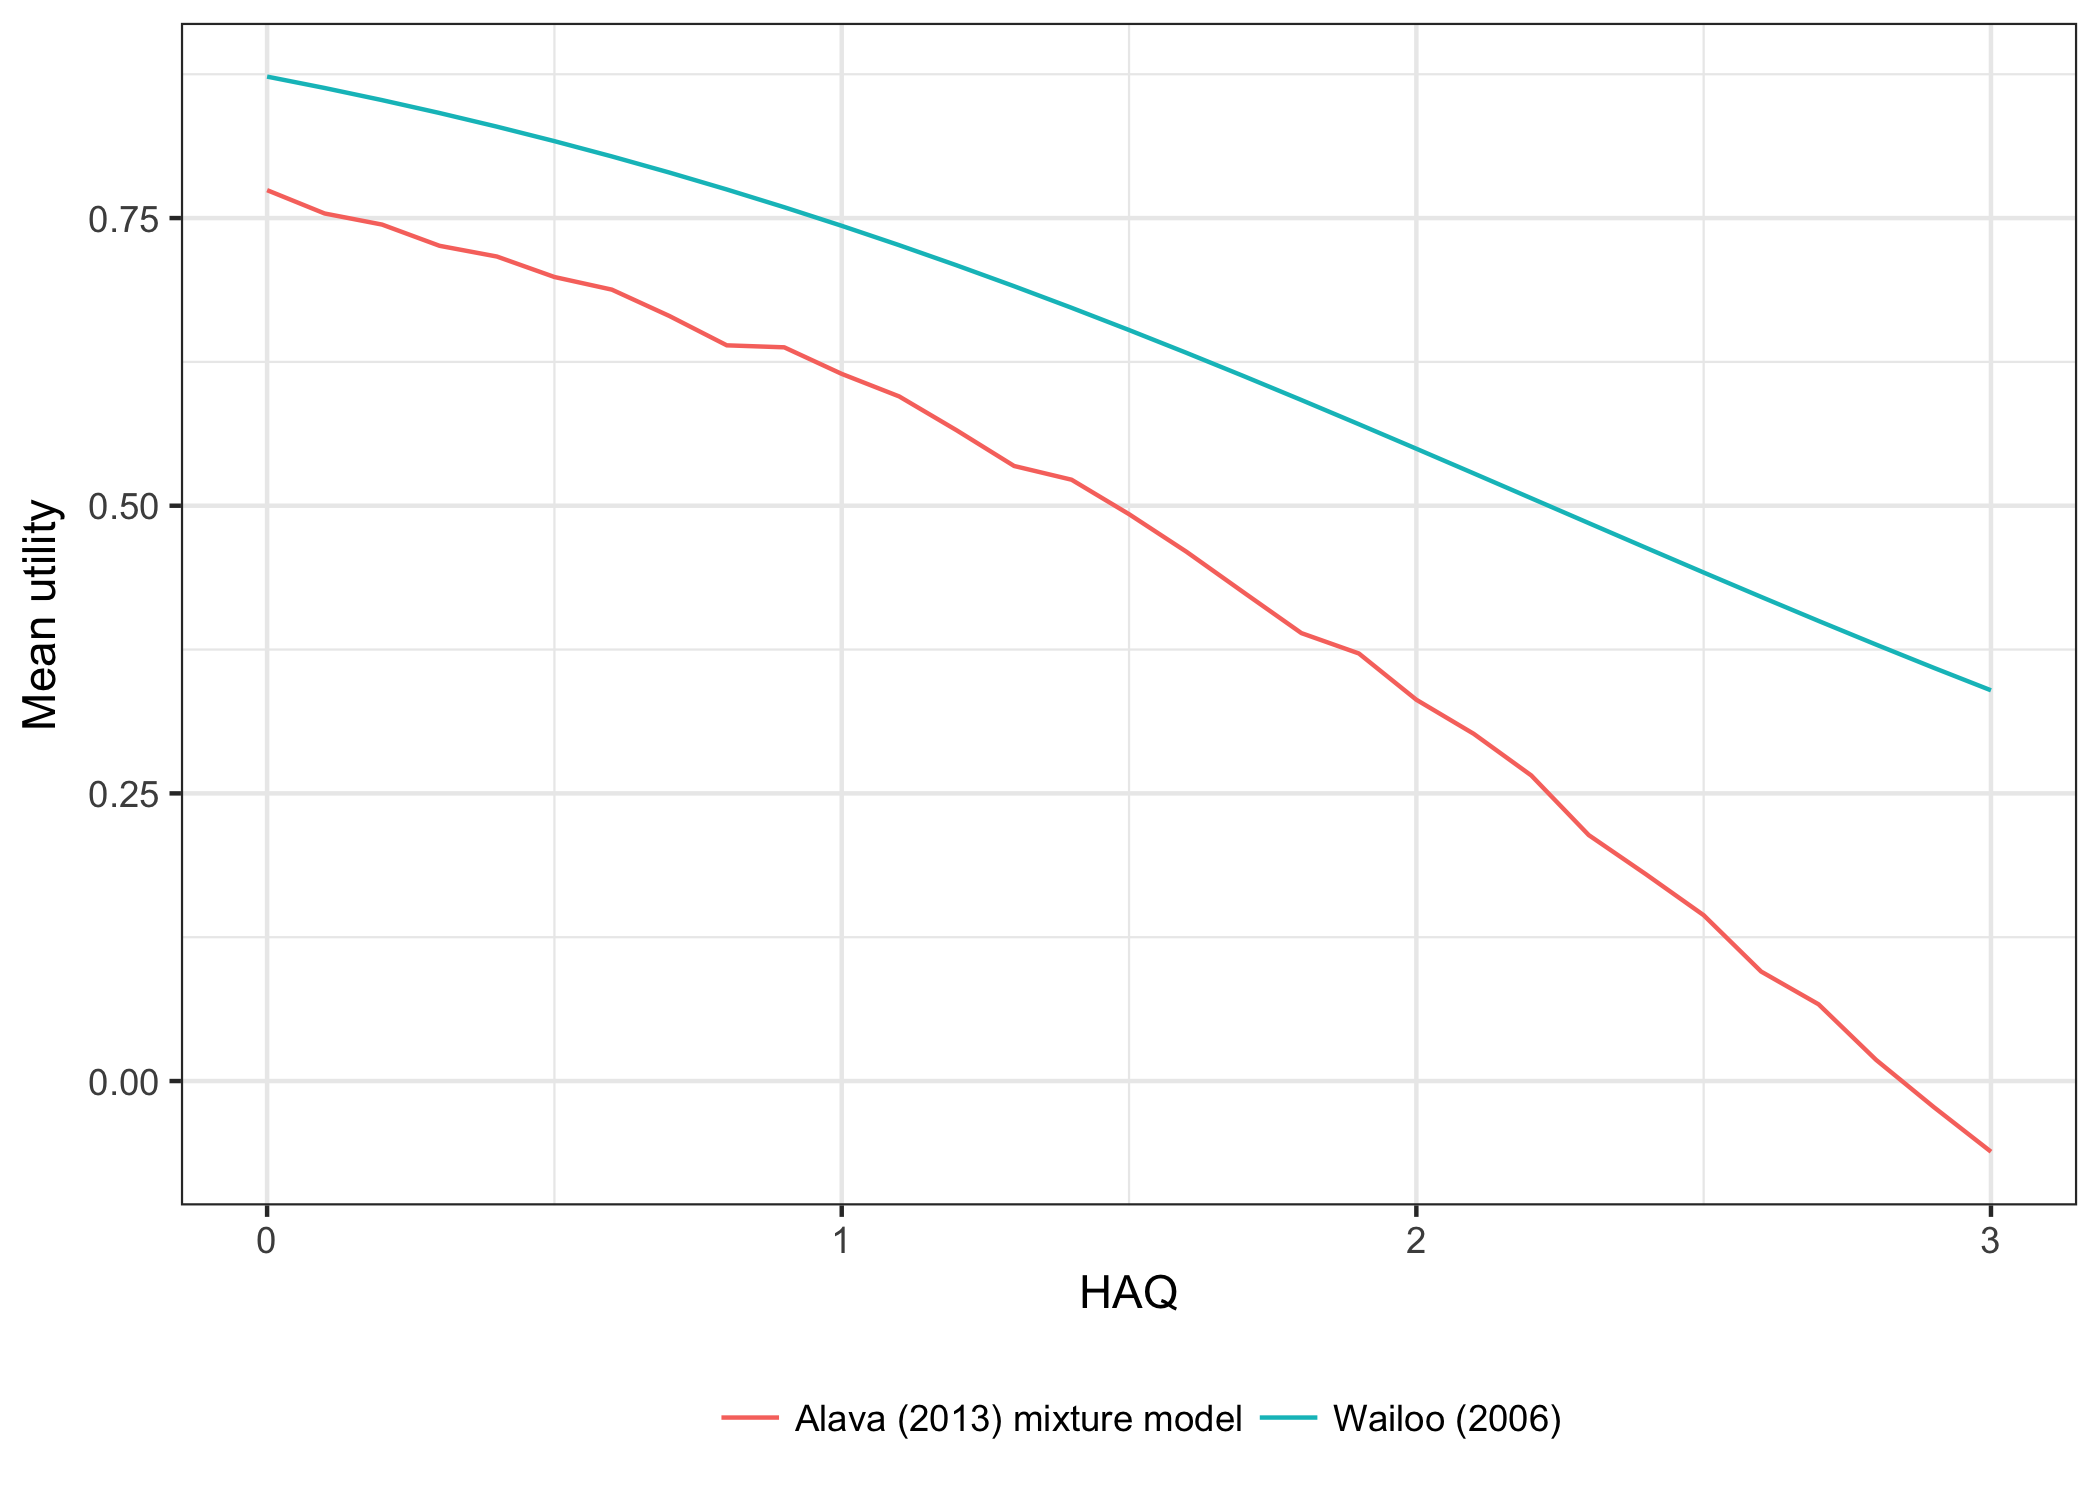
\includegraphics[max size={.8\textwidth}{.8\textheight}]{figs/util-byhaq-comparison.png}
\caption{Simulated mean utility by current
HAQ}\label{fig:util-comparison}
\end{figure}

The utility score depends on serious infections in addition to HAQ. In particular, disutility due to serious infections is assumed to be 0.156 for the duration of the month of infection based on prior studies \citep{stevenson2016adalimumab, oppong2013impact}. However, given the weak evidence for this estimate, the disutility of an infection is allowed to vary by 20\% in either direction.

Finally, in the \R{} package, we also allow users to incorporate treatment attributes unrelated to safety or efficacy that might impact utility. In particular, users can specify a vector of variables and a vector of corresponding coefficients. Each coefficient is the impact of the corresponding variable on utility in a given 6 month period. By default, we include variables related to mode of administration (infusion, injection, oral) and years since FDA approval; however, since we have no evidence on the impact of each variable on utility, the coefficients are set to 0 in our default settings.  

\subsection{Mortality}
The probability of death is simulated as a function of age/sex specific mortality from U.S. lifetables \citep{arias2015united}, baseline HAQ, and changes in HAQ from baseline. \citet{wolfe2003predicting} estimate an odds ratio for the effect of HAQ on mortality of 2.22, which is applied to the absolute mortality rates of the general population (HAQ score of 0). To capture the effect of treatment on mortality, we assume that, for every 0.25-unit increase in HAQ score, subsequent 6-month mortality increases according to the hazard ratios reported in \citet{michaud2012mortality}. Parameter estimates are shown in \autoref{tbl:mortpars}.


\begin{table}[!ht]
\begin{center}
\begin{threeparttable}
\caption{Mortality parameters} \label{tbl:mortpars}
\footnotesize
\begin{tabularx}{\textwidth}{@{\extracolsep{\fill}}lcccc}
\hline
\multicolumn{2}{l}{} & \multicolumn{2}{c}{95\% CI} & \multicolumn{1}{l}{} \\
\cmidrule{3-4} 
\multicolumn{1}{l}{} & \multicolumn{1}{l}{Estimate} & \multicolumn{1}{c}{Lower} & \multicolumn{1}{c}{Upper} & \multicolumn{1}{c}{Reference} \\
\hline
Impact of baseline HAQ on mortality \\
\ExpandableInput{tables/mort-or.txt}
Impact of 0.25-unit change in HAQ from baseline on mortality\\
\ExpandableInput{tables/mort-hr-haqdif.txt}
\hline
\end{tabularx}
\scriptsize
Notes: 95\% confidence intervals are calculated using normal distributions on the log odds
and log hazard ratio scales. 
\end{threeparttable}
\end{center}
\end{table}


\autoref{fig:surv} plots survival curves by gender for $1,000$ patients with a baseline age of 55. Survival was simulated by setting the log odds ratios and log hazard ratios from \autoref{tbl:mortpars} equal to their point estimates. Three scenarios are considerd. In scenario one, patients do not have RA (i.e., HAQ score of 0). In the second scenario, patients have baseline HAQ score of 1 but it does not increase over time. In the third scenario, patients still have a baseline HAQ score of 1, but it increases by 0.03 per year. The third scenario, therefore, utilizes the relationship between changes and HAQ and mortality from \citet{michaud2012mortality} while the second scenario does not. 

Mean survival for females without RA was 82.5 years and declined to 77.0 for females with a constant baseline HAQ of 1 and to 72.4 when HAQ increased by 0.03 per year. Mean survival for males in the first, second, and third scenario were 79.4, 73.2, and 70.1 years respectively. Overall, the figure suggests that RA increases mortality and that larger increases in HAQ over time increase mortality by even more.

\begin{figure}[H]
\centering
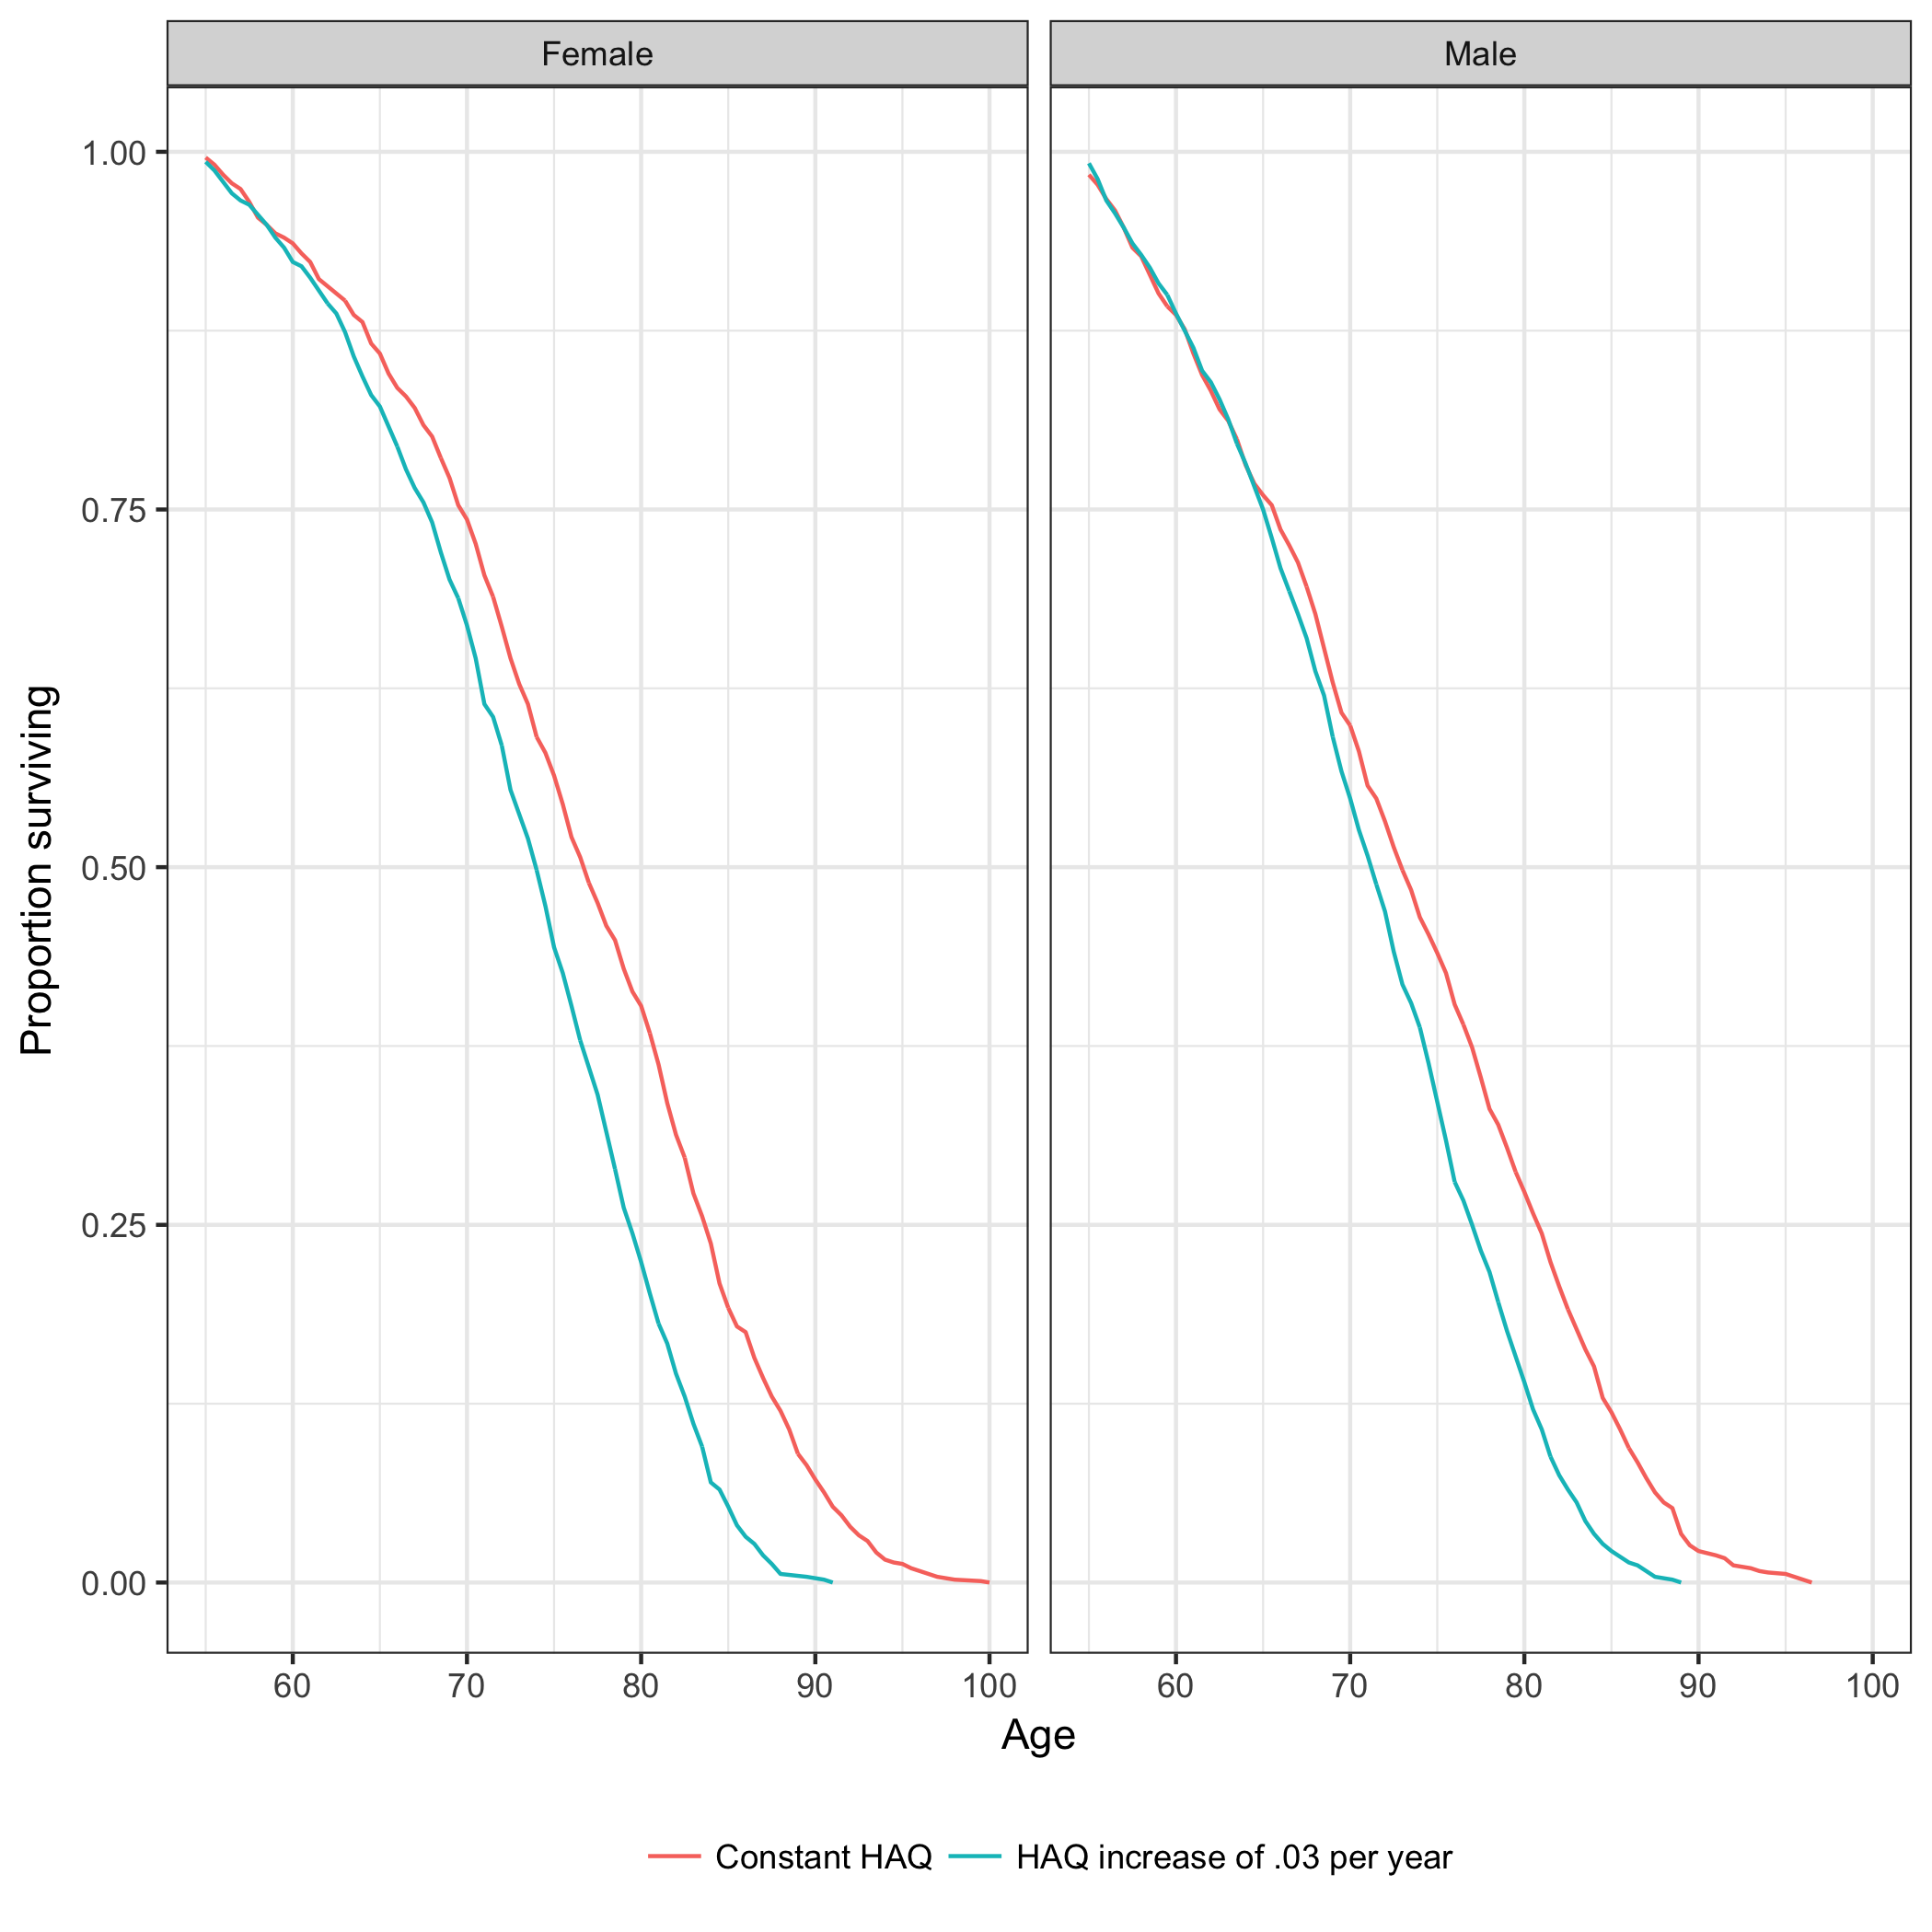
\includegraphics[max size={.7\textwidth}{.7\textheight}]{figs/surv.png}
\caption{Simulated survival curve for a patient age 55}\label{fig:surv}
\begin{minipage}{\linewidth}
\footnotesize
Notes: Baseline HAQ is 1 for the ``Constant HAQ'' and ``HAQ increase of 0.03 per year'' scenarios; baseline HAQ is 0 for the ``No RA'' scenario.
\end{minipage}
\end{figure}

\FloatBarrier

\subsection{Costs}\label{cost}

An overview of drug acquisition and administration costs is presented in \autoref{tbl:treat-cost}. Costs are a function of dose and frequency of administration, strength and dosage form, price, and infusion costs. Since infliximab dosing depend on patient weight, the costs for infliximab reported in the table average over a patient population that is 21\% male. The prices in the table are based on the wholesale acquisition cost (WAC) and do not include discounts or rebates so they may be higher than actual drug costs. In the simulation, a unique discount can be used for each drug; currently the discount is assumed to range from 20\% to 30\%. The methodology used to calculate drug acquisition and administration costs is described in more detail in \autoref{app:treat-cost}. 

\begin{sidewaystable}
\begin{center}
\begin{threeparttable}
\caption{Drug acquisition and administration cost} \label{tbl:treat-cost}
\scriptsize
\begin{tabular}{p{0.15\linewidth}p{0.15\linewidth}p{0.15\linewidth}rrrrrr}
\hline
\multicolumn{1}{p{0.15\linewidth}}{Drug} &
\multicolumn{1}{p{0.15\linewidth}}{Dose and frequency of administration} & 
\multicolumn{1}{p{0.15\linewidth}}{Strength and dosage form} & 
\multicolumn{1}{p{0.05\linewidth}}{Number of doses first 6 months}  & 
\multicolumn{1}{p{0.08\linewidth}}{Number of doses per year beyond the first 6 months} & 
\multicolumn{1}{c}{Price per unit} & 
\multicolumn{1}{c}{Infusion cost} & 
\multicolumn{1}{p{0.08\linewidth}}{Cost for the first 6 months} &
\multicolumn{1}{p{0.08\linewidth}}{Cost per year beyond the first 6 months}\\
\hline
\ExpandableInput{tables/treat-cost.txt}
\hline
\end{tabular}
\tiny
Notes: Costs in the table do not include rebates or discounts, but rebates and discounts are used in the simulation. Cost for infliximab are calculated by assuming that 21\% of patients are male and that the weight of men and women are 89 kg and 75 kg respectively. Tocilizumab is dosed weekly if weight is greater than 100 kg; costs for tocilizumab reported in the table are for patients weighing less than 100 kg. IV = intravenous; SC = subcutaneous. 
\end{threeparttable}
\end{center}
\end{sidewaystable}



Parameters associated with resource use are show in in \autoref{tbl:resource-use-pars}. Costs related to physician visits, chest X-rays, tuberculosis tests, and outpatient follow-up are based on \citet{claxton2016economic}. The cost per hospital day and the relationship between the HAQ score and the annual number of hospital days are from \citet{carlson2015economic}. Cost of any serious infection are assumed to be equal to the cost of pneumonia hospitalization at \$5,873, based on Medicare reimbursement rates. \citet{wolfe2005household} provide an estimate of annual income loss in relation to HAQ scores: \$4,372 (95\% CI: 2,078 to 6,607; 2002 dollars) change per unit HAQ change, which are inflated to 2019 dollars.


\begin{table}[H]
\begin{center}
\begin{threeparttable}
\caption{Resource use parameters} \label{tbl:resource-use-pars}
\footnotesize
\begin{tabularx}{\textwidth}{@{\extracolsep{\fill}}lcccc}
\hline
\multicolumn{2}{l}{} & \multicolumn{2}{c}{95\% CI} & \multicolumn{1}{l}{} \\
\cmidrule{3-4} 
\multicolumn{1}{l}{} & \multicolumn{1}{l}{Estimate} & \multicolumn{1}{c}{Lower} & \multicolumn{1}{c}{Upper} & \multicolumn{1}{c}{Reference} \\
\hline
Days in hospital per year \\
\ExpandableInput{tables/hosp-days-haq.txt}
\ExpandableInput{tables/hosp-cost-perday.txt}
General management cost \\
\ExpandableInput{tables/mgmt-cost.txt}
Productivity loss \\
\ExpandableInput{tables/prod-loss.txt}
\hline
\end{tabularx}
\scriptsize
Notes: 95\% confidence intervals for hospital days per year by HAQ score and hospital cost per day are calculated by using the methods of moments to generate the parameters of the gamma distribution given a mean and standard error. The 95\% confidence intervals for general management costs are based on normal distributions as assumed in \citet{claxton2016economic}. 95\% confidence interval for productivity loss are calculated using a normal distribution and inflated to 2016 dollars. 
\end{threeparttable}
\end{center}
\end{table}

\subsection{Insurance value}
In the IVI-RA Model interface, users have complete control over the probability of illness parameter and the marginal rate of substitution between the sick and the well states. In the IVI-RA Value Tool, we set the probability of obtaining RA in the next year equal to $0.000633$, based on the annual incidence rate reported for individuals age 55 to 64 in \citet{myasoedova2010incidence}. Furthermore, we set the the marginal rate of substitution between the sick and well states equal to 1.5 given that positive demand for health insurance suggests that it is positive, but note that there is considerable uncertainty around this estimate and that more research is required.  

\section{Simulation and uncertainty analysis}\label{sec:sim-uncertainty}

\subsection{Individual patient simulation}\label{individual-patient-simulation}

The IPS is a discrete-time simulation that simulates individual patients one at a time. Model cycles, denoted by $t$, were chosen to be 6-months long to be consistent with most RCT and real-world data evidence. \autoref{alg:IPS} describes the main components of the IPS for a single patient and a single treatment. The full simulation cycles through each treatment in a treatment sequence and through each simulated patient.

\begin{algorithm}
\caption{Main components of the individual patient simulation}
\label{alg:IPS}
\begin{enumerate}
\item \textbf{First 6 months ($t = 0$)}
\begin{enumerate}
\item Simulate treatment switching using \textbf{S1-S6}, time to serious infection $T_{si}$, and death (\autoref{ssec:simulating-death}).
\begin{enumerate}
\item \textbf{If} \textbf{S1-S6} leads to a treatment switch or if the sampled time to serious infection occurs during cycle 0 (i.e., $T_{si} = 0$), \textbf{then} stop treatment. It is assumed that HAQ does not change.
\newline \textbf{Else}, continue treatment. Simulate change in HAQ using \textbf{H1-H3} and time to treatment discontinuation $T$.
\item \textbf{If} patient died, \textbf{then} move to next patient. 
\end{enumerate}
\end{enumerate}
\item \textbf{Maintenance phase} (for $t > 0 \text{ and } t \leq T$)
\begin{enumerate}
\item Simulate death and change in HAQ.
\item \textbf{If} patient died, \textbf{then} move to next patient.
\item \textbf{If} $t = T$, \textbf{then} switch treatment. Treatment switch caused by a serious infection if time to serious infection occurred during or before cycle T (i.e., $T_{si} \leq T$). 
\end{enumerate}
\end{enumerate}
\end{algorithm}

\subsection{Parameter uncertainty}\label{parameter-uncertainty}
Parameter uncertainty is quantified using PSA, which propagates uncertainty in the model input parameters throughout the model by randomly sampling the input parameters from their joint probability distribution \citep{baio2015probabilistic, claxton2005probabilistic}. Probability distributions are determined according to the distributional properties of the statistical estimates, which, in turn, depend on the statistical techniques used and the distributions of the underlying data. We use normal distributions for sample means, gamma distributions for right-skewed data (e.g., hospital costs), and Dirichlet distributions for multinomial data. The multivariate normal distribution is used for regression parameters estimated using frequentist techniques, provided that the variance-covariance from the statistical analysis is available. For parameters estimated using a Bayesian NMA, we fit multivariate normal distributions to the posterior distribution of the parameters generated from the Markov-Chain Monte-Carlo (MCMC) algorithm using sample means and the sample covariance matrix. When we lack evidence on a parameter, we typically assume a uniform distribution with lower and upper limits that reflect the degree of uncertainty in the parameter. The PSA parameter distributions are summarized in \autoref{tbl:psa-dists}. 

\begin{table}[!ht] 
\begin{center}
\begin{threeparttable}
\caption{Probabilistic sensitivity analysis parameter distributions} \label{tbl:psa-dists}
\def\arraystretch{1.5}
\begin{tabularx}{\textwidth}{@{\extracolsep{\fill}}p{.65 \linewidth}p{.35 \linewidth}}
\hline
\multicolumn{1}{l}{Parameter(s)} & \multicolumn{1}{l}{Distribution} \\
\hline
Rebound factor & Uniform\\
NMA parameters - ACR response & Multivariate normal \\
NMA parameters - DAS28 & Multivariate normal \\
NMA parameters - HAQ & Multivariate normal \\
Drug acquisition and administration cost & Fixed \\
Survival model parameters for treatment duration during maintenance phase & Multivariate normal \\
US lifetable mortality rates & Fixed \\
Mortality probability odds ratio - baseline HAQ & Normal \\
Mortality probability hazard ratio - change in HAQ from baseline & Normal\\
ACR response to EULAR response mapping & Dirichlet \\
ACR response to SDAI mapping & Uniform \\
ACR response to CDAI mapping & Uniform \\
ACR response to HAQ mapping & Normal \\
EULAR response to HAQ mapping & Normal \\
Linear HAQ progression - by therapy & Normal \\
Linear HAQ progression - by age & Normal \\
Latent class growth model for HAQ progression & Normal \\
Utility model - \cite{alava2013relationship} mixture model & Multivariate normal \\
Utility model - \citet{wailoo2006modeling} & Normal \\
Hospital costs - hospital days by HAQ & Gamma \\
Hospital costs - hospital costs per day & Gamma \\
General management cost & Gamma \\
Serious infection - survival parameters & Normal \\
Serious infection - cost per infection & Uniform \\
Serious infection - utility loss & Uniform \\
\hline
\end{tabularx}
\scriptsize
%Notes: 
\end{threeparttable}
\end{center}
\end{table}


\subsection{Structural uncertainty}\label{stuctural-uncertainty}
We consider structural uncertainty due to two factors:

\begin{itemize}
\item The relationship between health states within the model.
\item The statistical model used to estimate parameters.
\end{itemize}

\autoref{tbl:competing-structures} summarizes the competing model structures, which are conditional on the perspective of the decision maker. In total, there are 12 x 2 x 8 x 2 = 384 possible model structures. The choice of model structure for the initial treatment phase (\textbf{H1-H3} and \textbf{S1-S6}) depends on the preferred measures of disease activity included in the model as well as whether statistical relationships should be modeled directly or indirectly. Likewise, model structures related to HAQ progression, treatment duration, and converting HAQ to utility all reflect uncertainty in the appropriate statistical model. 

\renewcommand{\arraystretch}{1.5}

\begin{table}[!ht]
\begin{center}
\begin{threeparttable}
\caption{Competing model structures} \label{tbl:competing-structures}
\begin{tabular}{p{0.80\linewidth}p{0.20\linewidth}}
\hline
\multicolumn{1}{c}{Component of model structure} & \multicolumn{1}{c}{Possible combinations} \\
\hline
Initial effect of treatment on HAQ (\textbf{H1-H3}) and switching (\textbf{S1-S6}) & 12  \\
HAQ trajectory & 2 \\
Cause and probability distribution used to model treatment discontinuation & 8 \\
Utility algorithm & 2 \\
\hline
\end{tabular}
\end{threeparttable}
\end{center}
\end{table}\renewcommand{\arraystretch}{1}


\subsection{Implementation}\label{implementation}
We begin by describing the simulation procedure conditional on model structure, which uses PSA to capture uncertainty within but not between models. The procedure proceeds in two steps: first, model parameters are sampled from their joint probability distribution (\autoref{parameter-uncertainty}), and second, for each parameter set, model outcomes are simulated one at a time for individual patients in the specified population (\autoref{sec:populations}).   

Analysts who wish to expand the analysis to capture uncertainty between models can follow the approach described in \citet{bojke2009characterizing}. In particular, for each randomly sampled parameter set, each model structure (or a subset of plausible model structures) can be simulated. The distribution of simulated outcomes across parameters and models will then reflect uncertainty both within and between models. 

It's important to note that simulation output for an individual patient captures differences in outcomes across patients due to random variation (often referred to as first order uncertainty). This information might be useful to patients since it is needed to predict the distribution of their future outcomes conditional on their characteristics, but less useful to a decision maker concerned with making treatment decisions for a population or subset of a population. Analysts wishing to use the model for CEA or MCDA should therefore estimate mean outcomes by averaging over the simulated patients for each parameter set and model structure. The number of simulated patients should be sufficiently large so that mean outcomes are stable across model runs (i.e., so that first order uncertainty is eliminated). 

Although CEA and MCDA is concerned with mean outcomes, that does not imply that it does not account for heterogeneity. Instead, since outcomes depend on the characteristics of each patient, model averages are a function of the population analyzed. Subgroup analyses can be used to examine differences in cost-effectiveness across subgroups by simulating patients with certain shared characteristics. 

Parameter and structural uncertainty imply decision uncertainty, or the degree to which decisions are made based on imperfect knowledge. Indeed, in CEA, with the aim to maximize health outcomes for a given budget, the optimal decision with current information is to choose the policy that maximizes the expected NMB; however, due to uncertainty, the incorrect policy may be considered the most cost-effective. To characterize uncertainty within a CEA framework, standard summary measures including 95\% credible intervals for NMBs and other model outcomes, cost-effectiveness planes, CEACs, the CEAF, and the EVPI can be calculated from the simulated output. Since the EVPI is computationally costly, it can be approximated using meta-modeling techniques \citep{jalal2013linear, jalal2015computing, heath2016estimating}.

\section{Validation}\label{sec:validation}
We aim to validate the model using the five types of validation described by \citet{eddy2012model}. Currently, we are able to use the first three validation types. First, we have checked the model for face validity by ensuring that simulated outcomes are consistent with current science and evidence. Second, we performed unit tests to verify that the individual units of code that are used to simulate the model return expected results. Third, we compared simulated results for key outcomes such as mortality, HAQ over time, and time to treatment discontinuation with real-world data and our underlying parameter values. In particular, we ran the model online under various scenarios using our R Shiny web application and checked the simulated outcomes. 

In the future, we plan to use both external validation and predictive validation to help fine tune our model. External validation will be performed by comparing outcomes simulated using our model to real-world outcomes and predictive validity will involve using our model to forecast future events and comparing our forecasted outcomes to the observed outcomes. 

\section{Limitations and areas for improvement}\label{sec:limitations}
The IVI-RA model is an open-source model that is part of the OSVP process and therefore designed to be updated and improved over time. We believe that there are number of potential areas for improvement.

\begin{itemize}
\item \textbf{Adverse events other than serious infections:} The current model does not account for side effects other than serious infections even though these are important to patients and can result in treatment switching. 
\item \textbf{Adverse events that vary across biologics:} The model allows the serious infection rate to differ between cDMARDs and tDMARDs but assumes that the infection rate is equal among tDMARDs. Future model versions might want to reconsider the evidence underlying this assumption.
\item \textbf{Time to treatment discontinuation:} Our time to treatment discontinuation curves are based on scanned data and combine information from multiple sources. Direct analyses of databases like the CORRONA database or the National Data Bank for Rheumatic Diseases (NDB) could generate more accurate estimates of treatment duration as well the effect of treatment response or disease activity level on discontinuation rates.  
\item \textbf{Patient preferences:} In the current model, patient utility is a function of the HAQ score and varies according to age, gender, and unobserved patient-specific factors. In other words, utility depends on treatment (through the effect of treatment on HAQ) and the characteristics of the patient. Future iterations of the model should consider other ways that treatment influences utility and that utility varies across patients. For example, disease activity level or the number of previous therapies might help predict utility conditional on HAQ. Furthermore, surveys could be used to estimate the effect of treatment attributes such as route of administration or frequency of administration on utility. Finally, since unobserved patient-specific factors are very important predictors of utility, the model could be run for specific classes of patients within the mixture model (e.g., subgroups where HAQ has the largest effect on utility), although it might be difficult to identify these patient subgroups in a real-world setting. 

\item \textbf{Treatment effect modifiers:} There is currently little evidence (that we are aware of) suggesting that treatment effects vary across patients. When there is sufficient evidence in the literature related to treatment response heterogeneity, we will allow treatment response at 6 months to depend on the characteristics of the patient.  
\item \textbf{Treatment effects after treatment failure:} There are two main limitations in the model related to reductions in treatment response after failing a biologic; first, there are not enough RCTs to reliably estimate tDMARD-specific treatment effects for tDMARD experienced patients using a NMA, and second, treatment response likely does not only depend on whether a patient is tDMARD naive or experienced, but on the number of previous failures as well. Our current approach is to assume that treatment response is reduced for tDMARD experience patients based on evidence from \citet{carlson2015economic}. One possible extension is to use a Bayesian NMA approach in which the \citet{carlson2015economic} results are used to generate priors for the tDMARD experienced group. As new RCTs become available, the posterior distributions from the Bayesian analysis would move further from the prior and closer to estimates from the trials. The estimates could be further improved by combing NMA results with real-world data and modeling reductions in treatment response as a flexible function of the number of failed biologics. 
\item \textbf{A LCGM for the progression of tDMARDs over time:} The LCGM can be used to model HAQ progression for patients using cDMARDs or on NBT; however, we only have estimates of constant linear progression of HAQ for patients on biologics. Future studies that use non-linear mixture models to model the long-term progression of disease for patients using tDMARDs are needed. 
\item \textbf{Long-term trends in disease activity:} The current model uses results from RCTs to model changes in disease activity during the first 6 months of treatment. But there is, to our knowledge, no evidence on the progression of disease activity over time. New studies are needed to model both the long-term impact of treatment on disease activity and the correlation between changes in disease activity and changes in HAQ.
\item \textbf{The patient population:} Our population characteristics are based on summary data reported in the published literature. As a result, the sampled patient populations within the model do not account for correlations across all of the variables. Distributions estimated from patient databases like the CORRONA database or the NDB would yield more realistic patient populations. 
\item \textbf{Estimating the rebound effect:} One of the most important predictors of cost-effectiveness is the degree to which the HAQ score increases following treatment failure. Most models currently assume that the HAQ score increases by the same amount as the initial 6 month decline in the HAQ score, but there is little evidence to support this. Studies that attempt to quantify the rebound effect are critical. 
\item \textbf{Insurance value:} Additional research is needed on insurance value and its use in value assessment. First, the framework presented here assumes that there is a single probability of illness and that treatment benefits and costs can be attributed to that sick state. However, in practice, the probability of illness depends on age and illness (e.g., RA) worsens over time. Moreover, in RA, treatment benefits and costs depend on disease severity. Future research should consider insurance value in a dynamic context, in which the value to a healthy individual today depends on the probability of all future health states. Second, new research is needed on the marginal rate of substitution between the sick and well states. \citet{lakdawalla2017insurance} suggest a few promising approaches.     
\end{itemize}

\begin{appendices}
\setcounter{table}{0}
\renewcommand{\thetable}{A\arabic{table}}
\setcounter{figure}{0}
\renewcommand{\thefigure}{A\arabic{figure}}
\setcounter{equation}{0}
\renewcommand{\theequation}{A\arabic{equation}}

\section{Rates, probabilities, and standard errors}\label{app:math}
\subsection{Using odds ratios to adjust probabilities}\label{app:odds-ratio-prob}
Let $p_1$ be a baseline probability, $\beta$ be a vector of log odds ratios, and $x$ be a vector of regressors. We apply the log odds ratios to $p_1$ to generate a new probability $p_2$ with the logistic equation,

\begin{align}
p_2 &= \frac{1}{1 + \exp\left[-\left(\logit(p_1) + x^T\beta \right)\right]},
\end{align}

where,

\begin{align}
\logit(p) = \log\left(\frac{p}{1-p}\right)
\end{align}

\subsection{Converting rates and probabilities}\label{app:rate-prob}
Given a \emph{constant} rate $r$ during a given time period, we estimate the probability of an event occurring before time $t$ using the exponential distribution,

\begin{align}
p(\tau < t |r) &= 1 - e^{-rt}.
\end{align}

Given a probability $p$, the rate parameter is recovered by applying the log transformation,

\begin{align}
r = \frac{-\ln(1-p)}{t}.
\end{align}

\subsection{Calculating standard errors from confidence intervals}\label{app:ci-se}
Journal articles often report confidence intervals rather than standard errors. However, given that regression coefficients are asymptotically normally distributed, standard errors can be calculated from a confidence interval using the normal distribution. In particular, given a coefficient estimate $\beta$ (e.g., a log hazard ratio, log odds ratio, or linear regression coefficient) and an upper bound $u$ and lower bound $l$ of a two-sided 95\% confidence interval, we calculate the standard error as,

\begin{align}
SE(\beta) = \frac{u - l}{2 \cdot \Phi^{-1}(0.975)},
\end{align}

where $\Phi^{-1}(p)$ is the quantile function of the normal distribution. 


\section{Heterogeneous populations}\label{app:population}
When generating heterogeneous patient populations, we sample binary variables from binomial distributions, continuous uncorrelated variables from normal distributions, and continuous correlated variables from multivariate normal distributions. Truncated distributions are used when variables are restricted to lie within certain intervals. 

In particular, the proportion of the female population is drawn from a binomial distribution while age, disease duration and the number of previous DMARDs are drawn from truncated normal distributions. Each sampled value of the number of previous DMARDs is rounded to the nearest integer. Baseline HAQ and three disease activity measures (DAS28, SDAI, and CDAI) are drawn from truncated multivariate normal distributions. The covariance matrix is calculated using the correlations reported in \citet{aletaha2005acute} (\autoref{fig:da-cor}).


\begin{figure}[H]
\centering
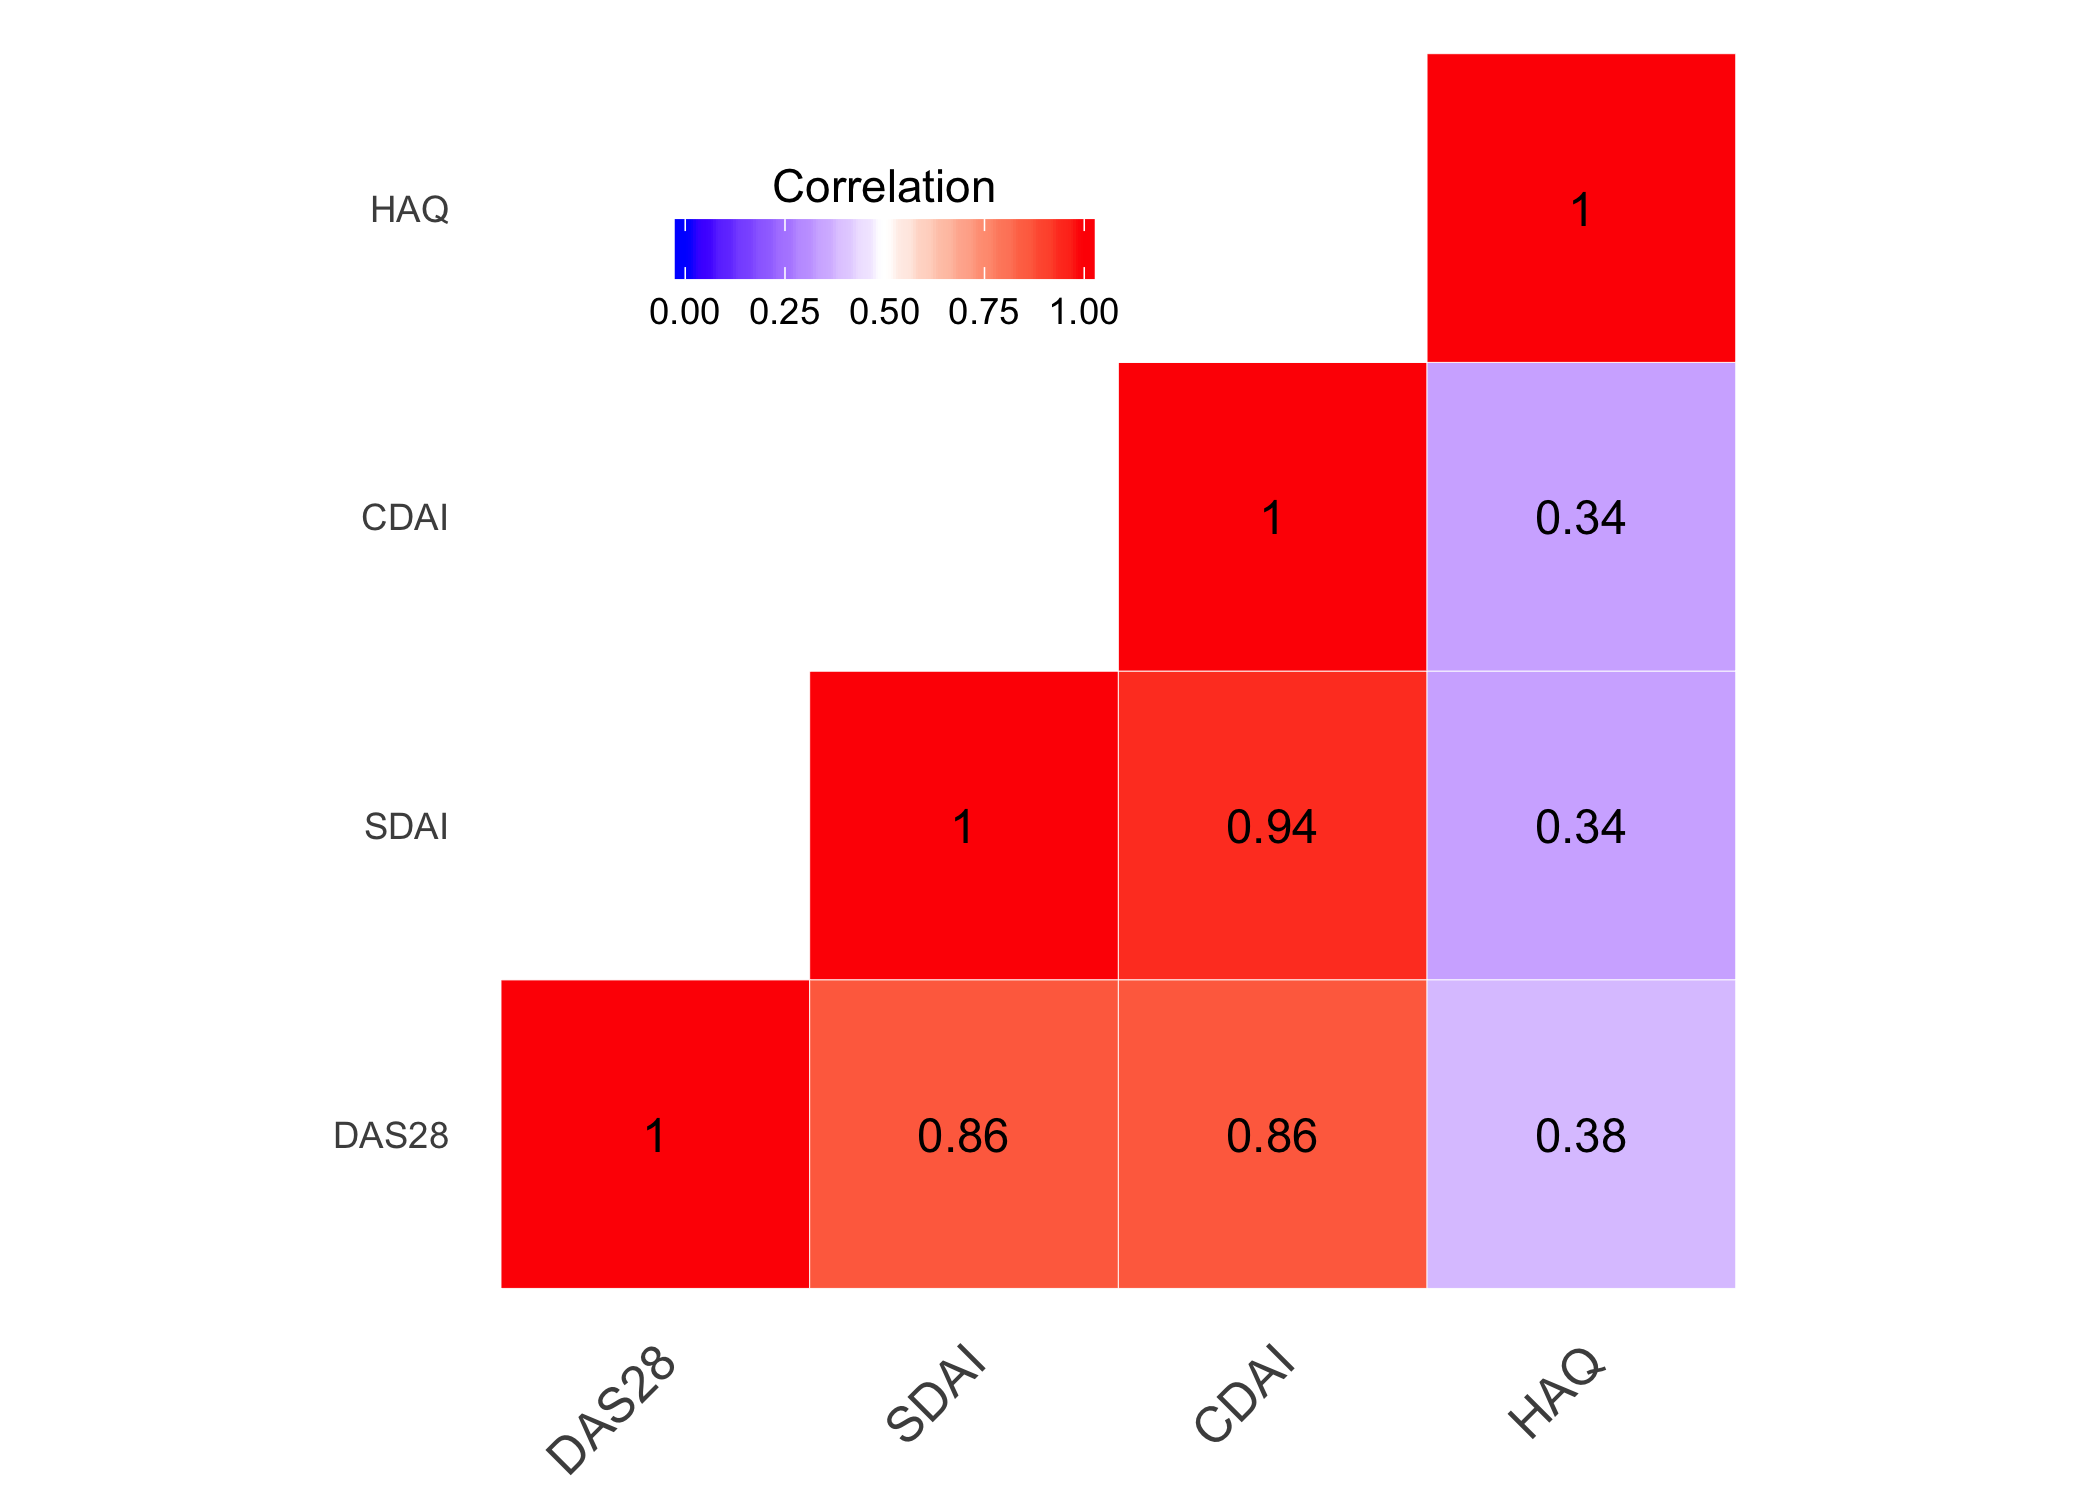
\includegraphics[max size={.7\textwidth}{.7\textheight}]{figs/da-cor.png}
\caption{Correlations between disease activity measures and HAQ}\label{fig:da-cor}
\end{figure}

We used the correlations from the routine cohort (during visit 1) rather than correlations in the inception cohort (at baseline) since the correlation between HAQ and the disease activity measures were more similar to those from the Leflunomide database \citep{smolen2003simplified}. That said, correlations between the three disease activity measures were nearly identical in each cohort. The one exception was that the correlation between SDAI and CDAI of 1 in the routine cohort seemed unreasonably high so we used the value of 0.94 from the inception cohort. 



We used this sampling procedure to simulate 1,000 patients. Summary statistics from a simulated patient cohort of size 1,000 are shown in \autoref{tbl:pats-samp}.

\begin{table}[!ht]
\begin{center}
\begin{threeparttable}
\caption{Summary of characteristics for 1,000 simulated patients} \label{tbl:pats-samp}
\begin{tabularx}{\textwidth}{@{\extracolsep{\fill}}lccc}
\hline
\multicolumn{2}{c}{} & \multicolumn{2}{c}{95 CI\%} \\
\cmidrule{3-4}
\multicolumn{1}{l}{} & \multicolumn{1}{c}{Mean} & \multicolumn{1}{c}{Lower} & \multicolumn{1}{c}{Upper}\\
\hline
\ExpandableInput{tables/pats-samp.txt}
\hline
\end{tabularx}
\scriptsize
\end{threeparttable}
\end{center}
\end{table}

\section{Mapping ACR response to changes in disease activity}\label{app-acr-da}
Let $DA$ denote disease activity, $n_1$ the number of patients with ACR 20 to <50 response, $n_2$ the number of patients with ACR 50 to <70 response, $n_3$ the number of patients with ACR $\geq$70 response, and $N$ the number of patients with an ACR response greater than or equal to 20\%. Mean changes in SDAI, CDAI, and DAS28 by overlapping ACR response categories are converted to mean changes by mutually exclusive ACR response categories as follows:

\begin{itemize}
\item \textbf{ACR 70}: Mean changes by ACR $\geq$70 were reported directly in \citet{aletaha2005simplified}.
\item \textbf{ACR 50 to <70}: Mean change in disease activity given ACR 50 to <70 response is calculated by solving for $\E[DA|50 \leq ACR < 70]$:

\begin{align}
\E[DA|ACR \geq 50] = \frac{n_2}{N} \cdot \E[DA|50 \leq ACR < 70]  + \frac{n_3}{N} \cdot \E[DA|ACR \geq 70].
\end{align}

\item Mean change in disease activity given ACR 20 to <50 response is calculated by solving for $\E[DA|20 \leq ACR < 50]$

\begin{align}
\E[DA|ACR \geq 20] = \frac{n_1}{N} \cdot \E[DA|20 \leq ACR < 50]  + \frac{n_2 + n_3}{N} \cdot \E[DA|ACR \geq 50].
\end{align}

\end{itemize}

\section{HAQ progression}\label{app:haq-progression}
\subsection{Effect of age on linear HAQ progression}\label{app:age-linear-haq}
\citet{michaud2011treatment} report an overall rate of linear HAQ progression and rates for three age groups (<40, 40-64, $\geq$ 65). Let $\beta$ be the overall rate of progression and $\beta_a$ be the rate of progression for age group $a$. To estimate the effect of age on the progression rate, we calculated the difference between the overall progression rate and the age specific rate, $\delta_a = \beta - \beta_a$. We estimated the standard error of this quantity assuming no covariance between $\beta$ and $\beta_a$,

\begin{align}
SE(\delta_a) = \sqrt{SE(\beta)^2 + SE(\beta_a)^2}.
\end{align}


\subsection{HAQ trajectory with a latent class growth model}\label{app:lcgm-haq}
\citet{norton2014health} model HAQ progression using a LCGM. The probability that individual $i$ is a member of class $c$ at time $t$ is modeled using a multinomial logistic regression,

\begin{align}
P(C_{it} = c) &= \frac{\exp(w_{it}^T\delta_c)}{\sum_{s=1}^{4}\exp(w_{it}^T\delta_s)},
\end{align}

where $\delta_s$ is the vector of regression coefficients associated with class $s$ and $w_{it}$ is the corresponding vector of regressors. The variables included in $w_{it}$ are age, gender, baseline DAS28, symptom duration, rheumatoid factor, ACR criteria, and socioeconomic status. Regression coefficients for classes 2-4 relative to class 1 are shown in \autoref{tbl:lcmm-class-coefs}. Older age and female gender are especially important predictors of membership in higher risk classes; a worse DAS28 score, rheumatoid factor positivity, fulfillment of the 1987 ACR criteria, lower socioeconomic status, and longer disease duration are also predictors of membership in classes with worse HAQ progression. 


\begin{table}[!ht] 
\begin{center}
\begin{threeparttable}
\caption{Determinants of class membership in the ERAS cohort} \label{tbl:lcmm-class-coefs}
\begin{tabularx}{\textwidth}{@{\extracolsep{\fill}}lccc}
\hline
\multicolumn{2}{l}{} & \multicolumn{2}{c}{95\% CI} \\
\cmidrule{3-4} 
\multicolumn{1}{l}{} & \multicolumn{1}{c}{Coefficient} & \multicolumn{1}{c}{Lower} & \multicolumn{1}{c}{Upper}  \\
\hline
\multicolumn{4}{@{}l}{\textbf{Class 2: moderate}} \\
\ExpandableInput{tables/lcgm-coef-class2.txt} \\
\multicolumn{4}{@{}l}{\textbf{Class 3: high}} \\
\ExpandableInput{tables/lcgm-coef-class3.txt} \\
\multicolumn{4}{@{}l}{\textbf{Class 4: severe}} \\
\ExpandableInput{tables/lcgm-coef-class4.txt}
\hline
\end{tabularx}
\scriptsize
Notes: Class 1, or the "low" group, is the reference category.
\end{threeparttable}
\end{center}
\end{table}

The HAQ trajectory for a given class can be written as,

\begin{align}\label{eqn:lcgm-haq}
y_{itc}^{*} &= \beta_{0c} + \beta_{1c}x_t + \beta_{2c}x_t^2 + \beta_{3c}x_t^3 + \epsilon_{it} \\
y_{itc} &= 
\begin{cases}
  0 & \text{if}\  y_{itc}^{*} < 0 \\
  y_{itc}^{*}& \text{if}\  0 \leq y_{itc}^{*} \leq 3 \\
   3 & \text{if}\  y_{itc}^{*} > 3 ,
\end{cases}
\end{align}

where $y_{itc}$ is the HAQ score, $x_t$ is a variable that is a function of time, the $\beta_{jc}$ are polynomial regression coefficients for members of class c, and $\epsilon_{it}$ is an error term.

Sam Norton generously provided us with statistical estimates of the 4 class LCGM used in \citet{norton2014health} from \href{https://www.statmodel.com}{MPlus}. Like \citet{stevenson2016adalimumab}, we noted that the coefficient estimates the MPlus resulted in large fluctuations in the predicted HAQ scores, likely because three decimal places was not precise enough for the cubic term in \autoref{eqn:lcgm-haq}. We consequently used the coefficient estimates to predict the probability of class membership---which are less likely to be influenced by the number of reported decimal places---but estimated \autoref{eqn:lcgm-haq} using the observed HAQ values reported in Figure 2 in \citet{norton2014health}. However, since standard errors were artificially high using grouped data, we standard errors in \autoref{eqn:lcgm-haq} were based on those reported in the original paper. Moreover, since we are only interested in the HAQ trajectory following the HAQ decline during the initial treatment phase, we limited our analysis to HAQ values from year 2 and onwards. Using the post year 2 data, we estimated \autoref{eqn:lcgm-haq} using separate linear regressions with cubic polynomials for each class (\autoref{tbl:lcmm-growth-coefs}). Like \citet{norton2014health}, we set $x_t$ equal to a reciprocal transformation of time,

\begin{align}
x_t &= 1 - \frac{1}{t+1}
\end{align}

\begin{table}[!ht] 
\begin{center}
\begin{threeparttable}
\caption{LCGM HAQ trajectory coefficients} \label{tbl:lcmm-growth-coefs}
\begin{tabularx}{\textwidth}{@{\extracolsep{\fill}}lccc}
\hline
\multicolumn{1}{l}{} & \multicolumn{1}{c}{Coefficient} & \multicolumn{1}{c}{Standard error}  \\
\hline
\multicolumn{3}{@{}l}{\textbf{Class 1: low}} \\
\ExpandableInput{tables/lcgm-coef-growth-class1.txt} \\
\multicolumn{3}{@{}l}{\textbf{Class 2: moderate}} \\
\ExpandableInput{tables/lcgm-coef-growth-class2.txt} \\
\multicolumn{3}{@{}l}{\textbf{Class 3: high}} \\
\ExpandableInput{tables/lcgm-coef-growth-class3.txt} \\
\multicolumn{3}{@{}l}{\textbf{Class 4: severe}} \\
\ExpandableInput{tables/lcgm-coef-growth-class4.txt}
\hline
\end{tabularx}
\scriptsize
Notes: Class 1, or the ``low'' group, is the reference category.
\end{threeparttable}
\end{center}
\end{table}

In the simulation model, we simulate the HAQ score at 6 months as a function of the baseline HAQ score and the change in HAQ during the initial treatment phase. Since the \citet{norton2014health} model is not conditional on the HAQ score in the previous period, we use it to predict changes in HAQ rather than the level of the HAQ score. More precisely, for a patient in a given class, we model the change in HAQ as,  

\begin{align}\label{eqn:lcgm-dhaq}
\Delta y_{itc}^{*} &= y_{i,t,c}^{*} - y_{i,t-1,c}^{*} \\
&= \beta_{1c}(x_t - x_{t-1}) + \beta_{2c}(x_t^2 - x_{t-1}^2) + \beta_{3c}(x_t^3-x_{t-1}^3) + (\epsilon_{i,t} - \epsilon_{i,t-1}). \nonumber
\end{align}

Since \autoref{eqn:lcgm-haq} was estimated on aggregated data, we did not have reliable estimates of $\epsilon_{it}$. We consequently set $\epsilon_{i,t} - \epsilon_{i,t-1}$ equal to 0, which implies that we are generating a mean response rather than a predicted response. In other words, we are not simulating the random variation associated with each individual, but are still accurately simulating mean outcomes across populations or subpopulations. 

\section{Simulating mortality}\label{ssec:simulating-death}
Death is simulated for each patient during each model cycle based on age, gender, baseline HAQ, and change in HAQ from baseline. A 0/1 death indicator is randomly drawn using the following procedure: 
\begin{enumerate}
\item Find $q_{xg}$, the probability that a patient of gender $g$ and age $x$ will die before age $x+1$, from lifetables.
\item As described in \autoref{app:odds-ratio-prob}, adjust $q_{gx}$ using the effect of a change in baseline HAQ on the odds of mortality, $OR$,
\begin{align}
p_m = \frac{1}{1 + \exp{\left[-(\text{logit}(q_x) + \log(OR)\cdot HAQ)\right]}}.
\end{align}
\item Following \autoref{app:rate-prob}, convert the mortality probability, $p_m$, into a mortality rate, $r_m$.
\begin{align}
r_m &= -log(1 - p_m).
\end{align}
\item Adjust the mortality rate, $r_m$, using the estimated log hazard ratio of mortality, $HR$, of a change in HAQ from baseline, $\Delta$ HAQ.
\begin{align}
r_m &= r_m \cdot \exp[\log(HR) \cdot \Delta HAQ]
\end{align}
\item Following \autoref{app:rate-prob}, convert the mortality rate into a probability given a 6-month cycle length,
\begin{align}
p_m = 1 - \exp[-r_m * (6/12)].
\end{align}
\item Randomly draw a 0/1 death indicator, $d$, given the probability of death, $p_m$,
\begin{align}
d \sim \text{Bin}(1, p_m).
\end{align}
\end{enumerate}

\section{Simulate utility}\label{app:utility}
\subsection{Mixture model}\label{app:sim-utility-mixture}
The mixture model estimated by \citet{alava2013relationship} simulates utility in two stages. In the first stage, we sampled pain for a given individual in a particular model cycle based on the HAQ score. In the second stage, we simulated utility as a function of HAQ, pain and age/sex.

\subsubsection{Simulating pain}
To simulate pain from HAQ, we used the summary statistics for pain and HAQ reported in \citet{sarzi2002correlation}. Pain was measured with the visual analog scale (VAS) with mean  $\mu_{pain} =$ 61.65 and standard deviation $\sigma_{pain} =$ 19.10, while HAQ was reported to have mean $\mu_{haq} =$ 1.39 and standard deviation $\sigma_{haq} =$ 0.59. 

We then estimated the correlation between pain and HAQ by digitally scanning the curve depicting the (linear) relationship between pain and HAQ (Figure 114) shown in \citet{stevenson2016adalimumab}. Using the scanned data, we regressed pain on HAQ using simple ordinary least squares (OLS). The correlation between pain and HAQ, estimated as $\rho =$ 0.52, was calculated by rearranging the OLS estimate for the slope, $\beta$, of the regression model,

\begin{align}
\rho = \beta \cdot \frac{\sigma_{haq}}{\sigma_{pain}}.
\end{align}

Pain was simulated using these parameters by assuming that pain was normally distributed conditional on HAQ,

\begin{align}
pain | haq = h \sim N\left (\mu_{pain} + \rho \frac{\sigma_{pain}}{\sigma_{haq}}(h - \mu_{haq}), \sigma^2_{pain}(1 - \rho^2)\right).
\end{align}

However, since the VAS is constrained to lie between 0 and 100, pain was drawn from a truncated normal distribution with a lower limit of 0 and an upper limit of 100. 

\subsubsection{Simulating utility}
After simulating pain, we simulated utility with a mixture model. Within each class $c$, the HAQ score for patient $i$ in period $t$ was modeled as,

\begin{align}
y_{it|C_{it}} &= 
\begin{cases}
  1 & \text{if}\  y^{*}_{it|C_{it}}>0.883 \\
  y^{*}_{it|C_{it}} & \text{otherwise}
\end{cases}\\
y^{*}_{it|C_{it}} &= \alpha_{ic} +  x_{it}^T\beta_{c} + \epsilon_{it}\\
\alpha_{ic} &=  \gamma_{c} + z_{i}^T\kappa + \mu_{i},
\end{align}

where $\epsilon_{it}$ is a random error term and $\beta_{c}$ is a vector of regression coefficients corresponding to the vector of variables $x_{it}$. $\alpha_{ic}$ is a random intercept for individual $i$ and class $c$ that is predicted by a class-specific intercept, $\gamma_c$, a vector of individual-specific variables $z_{i}$, a coefficient vector $\kappa$, and an error term, $\mu_i$. Variables included in $x_{it}$ are $HAQ$, $HAQ^2$, $Pain/100$, $Age/10$, and $Age/100$; $z_{i}$ contains a single indicator variable, $Male$, equal to 1 if the patient is male and 0 if female.

The probability of class membership was modeled using a multinomial logit model,

\begin{align}
P(C_{it} = c) &= \frac{\exp(w_{it}^T\delta_c)}{\sum_{s=1}^{4}\exp(w_{it}^T\delta_s)},
\end{align}

where there are four possible classes and $\delta_c$ is a vector of coefficients corresponding to the vector of variables, $w_{it}$ (which includes an intercept). Variables included in $w_{it}$ other than the intercept are $HAQ$, $Pain/100$, and $Pain/100^2$.

We sampled from the mixture model as follows.

\begin{enumerate}
\item For each individual $i$, sample the error term, $\mu_{i} \sim N(0, \sigma^2_\mu)$.
\item For each individual $i$ and time-period $t$: 
\begin{enumerate}
\item Sample class membership conditional on $w_{it}$; that is, sample $C_{it} \sim \Cat(p_1, p_2, p_3, p_4)$ where $p_c$ is the probability of being in class $c$.
\item Predict the intercept $\alpha_{ic}$.
\item Sample the error term, $\epsilon_{it} \sim N(0, \sigma^2_\epsilon)$.
\item Predict the HAQ score, $y_{it}$. 
\end{enumerate}
\end{enumerate}

\subsection{Logistic regression model}\label{app:sim-utility-logistic}
\citet{wailoo2006modeling} use a logistic regression equation to predict utility as a function of patient demographics, disease history, and current disease status. The regression coefficients from the model are shown in \autoref{tbl:util-wailoo-coef} and used to predict utility with the inverse logit function. Specifically, if the vector of coefficients is denoted by $\beta$ and the corresponding vector of explanatory variables is denoted by the vector $x$, then predicted utility is given by $1/(1 + \exp(-x^T\beta))$.


\begin{table}[!ht]
\begin{center}
\begin{threeparttable}
\caption{Logistic regression coefficient from Wailoo utility algorithm} \label{tbl:util-wailoo-coef}
\begin{tabularx}{\textwidth}{@{\extracolsep{\fill}}lcc}
\hline
\multicolumn{1}{c}{} & \multicolumn{1}{c}{Estimate} & \multicolumn{1}{c}{Standard error}  \\
\hline
\ExpandableInput{tables/util-wailoo-pars.txt}
\hline
\end{tabularx}
\scriptsize
Notes: Coefficients are from the logistic regression reported in \citet{wailoo2006modeling}. 
\end{threeparttable}
\end{center}
\end{table}

\section{Drug acquisition and administration costs}\label{app:treat-cost}

Drug acquisition and administration costs are calculated separately during the initial treatment phase and the maintenance phase since dosing typically differs. Costs are separated into acquisition costs and infusion costs. Infusion costs are calculated by multiplying the number of doses in a 6 month period by the cost of an infusion and acquisition costs are calculated as,

\begin{align}
cost = \left\lceil\frac{dose_{amt}}{strength_{amt}}\right\rceil \cdot doses_{num} \cdot price,
\end{align}

where $\lceil\cdot\rceil$ is the ceiling function and implies that products cannot be reused after opening, $dose_{amt}$ is the recommended dose of the drug, $strength_{amt}$ is the strength of the drug, $doses_{num}$ is the number of doses in a 6 month period, and $price$ is the price per unit of the treatment after discounts and rebates. For example, as shown in \autoref{tbl:treat-cost}, both the strength and the dose of adalimumab are 50 mg, so costs (before discounts and rebates) for the initial 6 month period are calculated by multiplying the number of doses (13) by the WAC (\$2,587.05).

When dosing depends on weight, costs are calculated separately for each patient in the simulation. In particular, costs are calculated as,

\begin{align}
cost &= \lceil weight \cdot dose_{amt}/strength_{amt}\rceil \cdot doses_{num} \cdot price,
\end{align}

where $weight$ is patient weight, $dose_{amt}$ is the dose per weight, and $strength_{amt}$, $price$, and $doses_{num}$ are defined in the same way as in the non-weight based scenario. To illustrate, the acquisition cost (before discounts and rebates) for infliximab after the first 6 months is calculated by multiplying each patient's weight by the dose (6 mg/kg) and dividing by the size of a vial (100 mg), and then multiplying by the number of doses (8.67) and the price per unit (\$1,167.82). 

\section{Annualized costs and benefits}\label{app:insurance-value}
Letting $t$ index time (in years), total costs ($\hat{cost}$) and QALYs ($\hat{qalys}$) for each patient simulated over a time horizon $T$ are given by,

\begin{align}
\hat{cost} &= \sum_{t=1}^T c_t \beta_c^t\\
\hat{qalys} &= \sum_{t=1}^T q_t \beta_q^t,
\end{align}

where costs and QALYs at time $t$, $c_t$ and $q_t$, are discounted using the discount factors $\beta_c$ and $\beta_q$, respectively. The discount factor is a function of the annual discount rate (typically assumed to be 0.03); that is, $\beta_s = 1/(1+r_s)$ where $r_s$ is the discount rate for $s=c,q$. The time horizon $T$ is set to equal the maximum number of years that a patient could survive within the model---currently the maximum age that a patient could survive to is 100 given the default lifetables used within the model, so $T$ is equal to 100 minus a patient's age at the start of the simulation. 

Annualized QALY gains and costs, which are used to estimate the annual insurance value of treatment, can therefore be calculated using the formula for a geometric series and assuming a constant flow rate each model cycle (that is, by setting $c_t = c$ and $q_t = q$ in each time period). In particular, annualized costs $c$ and QALYs $q$, can be derived by solving the following equations for $c$ and $q$,  

\begin{align}
\hat{cost} = c \frac{1-\beta_c^T}{1- \beta_c}\\
\hat{qalys} = q \frac{1-\beta_q^T}{1- \beta_q}.
\end{align}

\section{Network Meta-Analysis}\label{appendix:NMA}
Treatment effects with tDMARDs relative to cDMARDs for moderate to severe RA patients who failed treatment with a conventional DMARD were estimated based on currently available evidence as reported in the literature. The two populations of interest were: 1) RA patients without a history of prior tDMARD treatment (tDMARD naive population); and 2) RA patient with a history of tDMARD treatment (tDMARD experienced population). Relevant randomized controlled trials were identified with a systematic literature review and treatment effects were estimated by means of a network meta-analysis.
\subsection{Systematic literature review to identify relevant studies}\label{systematic-literature-review}
\subsubsection{Eligibility criteria}
Study eligibility criteria were defined in terms of the population, interventions, comparisons, outcomes, and study design (PICOS).

\begin{table}[!ht]
\begin{center}
\scriptsize
\begin{threeparttable}
\caption{Study eligibility criteria} \label{tbl:study-eligibility}
\begin{tabular}{p{0.20\linewidth}p{0.80\linewidth}}
\hline
\multicolumn{1}{l}{Criteria} & \multicolumn{1}{l}{Description}\\
\hline
Population & Adult (>18) patients with moderate to severe active rheumatoid arthritis who failed treatment with a conventional DMARD and were either targeted DMARD naive or experienced. \\
&\\
Interventions & Approved dosing regimens (or equivalent) of the following tDMARDs as monotherapy or in combination with a cDMARD: adalimumab, certolizumab pegol, etanercept, golimumab, infliximab, rituximab, abatacept, tocilizumab, sarilumab, anakinra, tofacitinib, baricitinib, upadacitinib, biosimilars; triple therapy (methotrexate, sulfasalazine, and hydroxychloroquine)\\

& \\
Comparators & cDMARDs; placebo; any of the interventions of interest; any other intervention (or dosing regimen) that facilitates an indirect comparison between the interventions of interest \\
&\\
Outcomes & At least one of the following outcomes at 6 months of follow-up: ACR 20/50/70, HAQ-DI, DAS28 \\
&\\
Study design & Randomized clinical trials \\
&\\
Other & Only full text reported in Enlgish were included. Studies only available as conference abstracts or presentations were excluded. \\
\hline
\end{tabular}
\scriptsize
\end{threeparttable}
\end{center}
\end{table}

\subsubsection{Literature search}
Relevant studies were identified by searching the following databases: Medline, EMBASE, and Cochrane Central Register of Controlled Trials. The searches were executed June 2017 with the following predefined search strategies and corresponding results.


\setlength\LTleft{0pt}
\setlength\LTright{0pt}

\subsubsubsection{Medline}

\begin{center}
\footnotesize
\begin{longtable}{@{\extracolsep{\fill}}rp{0.70\linewidth}r}
\caption{Medline literature search strategy} \label{tbl:medline-search} \\
\hline
\multicolumn{1}{r}{Order} & \multicolumn{1}{c}{Search terms} & \multicolumn{1}{r}{Results}  \\
  \hline 
\endfirsthead
  \caption[]{Medline literature search strategy}\\
  \hline
\multicolumn{1}{r}{Order} & \multicolumn{1}{c}{Search terms} & \multicolumn{1}{r}{Results}  \\
  \hline
\endhead
\hline
\multicolumn{2}{l}{Continued on next page}\\
\endfoot
\endlastfoot
\ExpandableInput{tables/medline-search.txt}
\hline
\end{longtable}
\end{center}

\subsubsubsection{Embase}

\begin{center}
\footnotesize
\begin{longtable}{@{\extracolsep{\fill}}rp{0.70\linewidth}r}
\caption{Embase literature search strategy} \label{tbl:embase-search} \\
\hline
\multicolumn{1}{r}{Order} & \multicolumn{1}{c}{Search terms} & \multicolumn{1}{r}{Results}  \\
  \hline 
\endfirsthead
  \caption[]{EMBASE literature search strategy}\\
  \hline
\multicolumn{1}{r}{Order} & \multicolumn{1}{c}{Search terms} & \multicolumn{1}{r}{Results}  \\
  \hline
\endhead
\hline
\multicolumn{2}{l}{Continued on next page}\\
\endfoot
\endlastfoot
\ExpandableInput{tables/embase-search.txt}
\hline
\end{longtable}
\end{center}

\subsubsubsection{Cochrane Central Register of Controlled Trials}

\begin{center}
\footnotesize
\begin{longtable}{@{\extracolsep{\fill}}rp{0.70\linewidth}r}
\caption{Cochrane Central Register of Controlled Trials literature search strategy} \label{tbl:cochrane-search} \\
\hline
\multicolumn{1}{r}{Order} & \multicolumn{1}{c}{Search terms} & \multicolumn{1}{r}{Results}  \\
  \hline 
\endfirsthead
  \caption[]{Cochrane Central Register of Controlled Trials literature search strategy}\\
  \hline
\multicolumn{1}{r}{Order} & \multicolumn{1}{c}{Search terms} & \multicolumn{1}{r}{Results}  \\
  \hline
\endhead
\hline
\multicolumn{2}{l}{Continued on next page}\\
\endfoot
\endlastfoot
\ExpandableInput{tables/cochrane-search.txt}
\hline
\end{longtable}
\end{center}

\subsubsection{Study selection}
Two investigators working independently scanned all abstracts identified in the literature search. The same two investigators independently reviewed relevant abstracts in full-text. Discrepancies occurring between the studies selected by the two investigators were resolved by involving a third investigator and reaching consensus.

\subsubsection{Data extraction}
Two investigators working independently extracted relevant data on study characteristics, interventions, patient characteristics, and outcomes from the final list of selected eligible studies. Discrepancies observed between the data extracted by the two investigators were resolved by involving a third investigator and reaching consensus.

\subsection{Analyses}\label{app:nma-analyses}
In order to perform a network meta-analysis where the risk of biased relative treatment effect estimates is limited we need to have 1) a single evidence network where each randomized controlled trial has at least one intervention in common with another trial; and 2) no differences in study designs and the distribution of patient characteristics that act as relative treatment effect-modifiers across the studies in the network (ref). For both the tDMARD naive population and the tDMARD experienced population a connected evidence network could be defined, however for the latter population the treatment history across studies was considered too different to obtain valid results from a network meta-analysis, and the limited number of studies would not allow adjusting for these differences with statistical techniques. Hence, network meta-analyses were only performed for the tDMARD naive population. Studies that reported results for a mixed population regarding prior tDMARD use were excluded from the analyses; only studies with results reported for a tDMARD naive population were included. 

Treatment effects at 6 months with each of the interventions in the network relative to cDMARDs were estimated in terms of ACR response, change from baseline in HAQ, and change from baseline in DAS28 with Bayesian random effects network meta-analysis models as presented by Dias et al. 2013. To avoid influencing the observed results by prior belief, uninformative prior distributions were used for the estimated treatment effect and between-study heterogeneity parameters. Posterior distributions for the model parameters are derived with the Markov chain Monte Carlo method using the JAGS software package (\url{http://mcmcjags.sourceforge.net/}). The studies included in each analysis for the tDMARD naive population were considered sufficiently similar regarding study design and distribution of patient characteristics that may act as relative treatment effect-modifiers. Accordingly, no meta-regression was performed to adjust for between-trial differences and the obtained estimated for each of the interventions were considered reflective of this target population of interest. 

\subsubsection{ACR response at 6 months}
The four mutually exclusive ACR response categories were estimated from the overlapping ACR categories using a ordered probit model appropriate for ordered categorical data \citep{dias2013evidence}. The model assumes that there is an underlying continuous variable (ACR20/50/70) categorized by specifying different cutoffs corresponding to the point at which an individual moves from one category to the next in each trial. The advantage of this approach over an analysis that considers ACR categories separately is that all possible outcomes are analyzed simultaneously based on the same randomized controlled trials, allowing for consistent estimates by category. 

More specifically, let $r_{jkl}$ be the number of patients in trial $j$ for treatment $k$ in the mutually exclusive category $l = 1,2,3,4$. The model can be written as,

\begin{align}
r_{jkl} \sim \Multinomial(p_{jk1}, p_{jk2}, p_{jk3}, p_{jk4}, n_{jk}),
\end{align}

where $p_{jkl}$ is the probability that a patient from trial $j$ and treatment $k$ is in category $l$ and there are $n_{jk}$ patients in trial $j$ and treatment $k$. Probabilities are modeled using a probit function,

\begin{align}
\Phi^{-1}(p_{jkl}) =
 \begin{cases}
     u_{jb} + z_{jl} & \text{ if } k = b \\
     u_{jb} + z_{jl} + \delta_{jbk} & \text{ if } k \succ b, \\
  \end{cases}
\end{align}

where $u_j$ is a trial specific intercept, $z_{jl}$ is a cutpoint for trial $j$ and category $l$, and $\delta_{jbk}$ is the effect of treatment $k$ relative to treatment $b$. The cutpoint for category $c$, $z_{jc}$, is modeled as random,

\begin{align}
z_{jc} \sim N(v_c, \sigma^2_z).
\end{align}

The study-specific relative treatment effects are also drawn from a common population distribution with mean $d_{bk}$ and variance $\tau^2$,

\begin{align}
\delta_{jbk} \sim N(d_{bk}, \tau^2),
\end{align}

where $d_{bk} = d_{Ak} - d_{Ab}$. To generate treatment responses, we estimate the response for treatment $A$ by averaging $\mu_{jA}$ across trials containing treatment $A$. In particular, letting $S_A = \{\mu_{1A}, \ldots \mu_{|S_A|A}\}$ be the set of all trials containing treatment $A$, we estimate,

\begin{align} \label{eqn:NMA-A}
A = \frac{1}{|S_A|}\sum_{\mu_{A} \in S_A} \mu_{A}.
\end{align}

We calculate the probability of ACR < 20\% improvement, ACR < 50\% improvement, and ACR < 70\% improvement with treatment $k$ as,

\begin{align}
P(ACR_k < 70) &= \phi(A + z_3 + d_{kA}) \\
P(ACR_k < 50) &= \phi(A + z_2 + d_{kA}) \\
P(ACR_k < 20) &= \phi(A + d_{kA}).
\end{align}

The probabilities of overlapping ACR response (i.e., ACR 20/50/70) are then,

\begin{align} \label{eqn:ACR-overlap}
P(ACR_k > 70) &= \gamma \cdot (1 - P(ACR_k < 70))\\
P(ACR_k > 50) &= \gamma \cdot  (1 - P(ACR_k < 50)) \\
P(ACR_k > 20) &= \gamma \cdot (1 - P(ACR_k < 20)),
\end{align}

where $\gamma$ is the reduction in treatment response at a given line of therapy. $\gamma = 1$ is a patient is bDMARD naive and on average, equal to .84 after failing a biologic. The mutually exclusive ACR response categories are easily derived from the overlapping categories. 

To avoid influencing the observed results by prior belief, uninformative prior distributions were used for the estimated model parameters. Posterior distributions for the model parameters are derived with the Markov chain Monte Carlo method.

\subsubsection{Change in HAQ and DAS28 at 6 months}
The models of changes in HAQ and DAS28 at 6 months use a normal likelihood (since the sample mean is approximately normally distributed by the central limit theorem if the sample size is reasonably large) and an identity link. 

More specifically, let $y_{jk}$ be the outcome of interest in trial $j$ and treatment $k$, and consider the model,

\begin{align}
y_{jk} \sim N(\theta_{jk}, \sigma^2_{jk}),
\end{align}

where,

\begin{align}
\theta_{jk} &=
 \begin{cases}
     \mu_{jb} & \text{ if } k = b \\
     \mu_{jb} + \delta_{jbk} & \text{ if } k \succ b.
  \end{cases}
\end{align}

$\delta_{jbk}$ is modeled using a random effect with $d_{AA} =0$,

\begin{align}
\delta_{jbk} \sim N(d_{bk}, \sigma^2),
\end{align}

where $d_{bk} = d_{Ak} - d_{Ab}$. As with the ACR response model, we allow treatment response to depend on patient characteristics by modeling $d_{bk}$ as a function of covariates for each individual patient $i$,

\begin{align}
d_{bk} &= x_{i}^T\beta_{bk},
\end{align}

In the simulation, we allow for treatment effect modifiers by modeling $d_{bk}$ as a function of covariates for each individual patient $i$,

\begin{align}
d_{bk} &= x_{i}^T\beta_{bk}.
\end{align}

The absolute treatment effect is estimated by calculating $A$ as in \autoref{eqn:NMA-A}. The absolute treatment effect for treatment $k$ is then,

\begin{align}
\gamma (A + d_{kA}),
\end{align}

where $\gamma$ is defined as in \autoref{eqn:ACR-overlap}. Uninformative priors were used to derive the posterior distributions.

\subsection{Evidence base}
\subsubsection{Study identification and selection}
\begin{figure}[H]
\centering
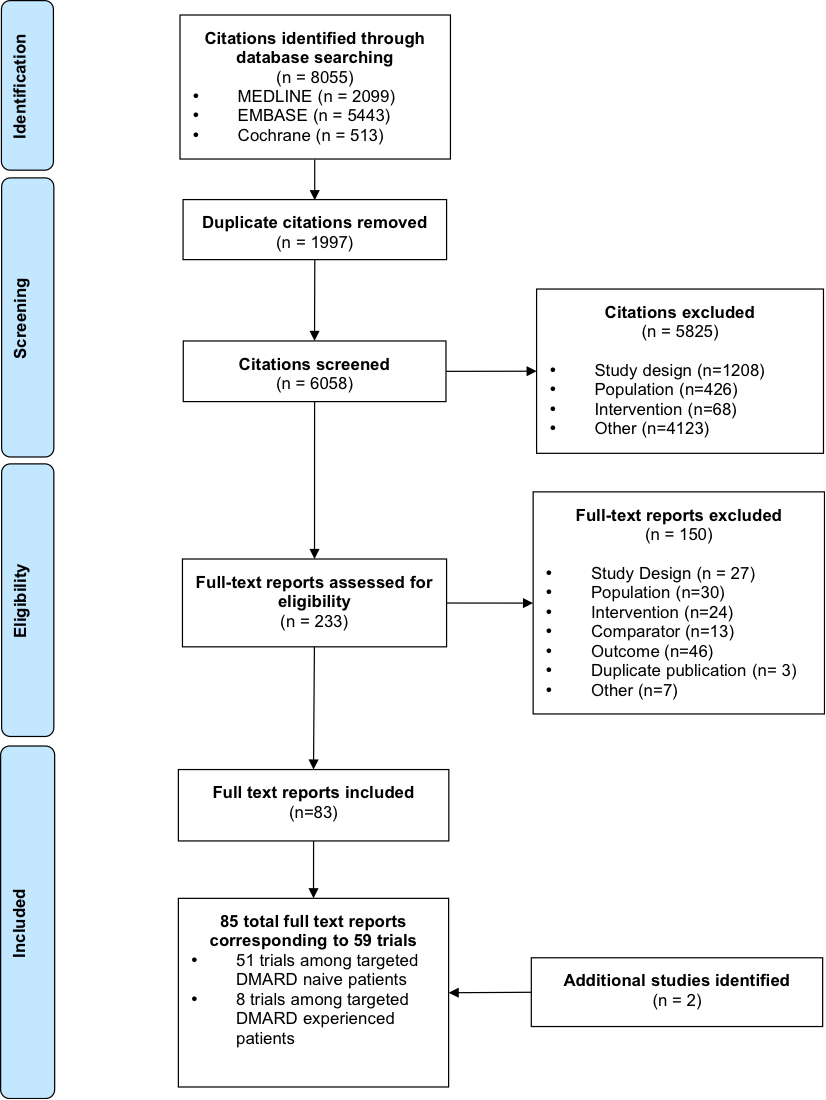
\includegraphics{study-selection.png}
\vspace*{10mm}
\caption{Study identification and selection}\label{fig:study-identification}
\end{figure}

\subsubsection{Included studies}




\begin{landscape}
\scriptsize
\begin{longtable}{p{2cm}p{2cm}p{10cm}p{4cm}}
\caption{Included studies and publications} 
\label{tbl:included studies} \\
\hline
\textbf{Trial ID}&\textbf{Author and Year}&\textbf{Title}&\textbf{Journal} \\
\hline
\endfirsthead
\hline
\textbf{Trial ID}&\textbf{Author and Year}&\textbf{Title}&\textbf{Journal} \\
\hline
\endhead
\hline 
\multicolumn{7}{l}{\emph{Continued on next page}} \\
\endfoot
\endlastfoot

\input{tables/included-studies.txt} \\
\hline 
\end{longtable}
\end{landscape}




\begin{landscape}
\scriptsize
\begin{longtable}{p{2cm}p{8cm}p{4cm}p{2cm}p{2cm}}
\caption{Excluded publications} 
\label{tbl:excluded-publications} \\
\hline
\textbf{Author and Year}&\textbf{Title}&\textbf{Journal}&\textbf{Reason}&\textbf{Subreason}& \\
\hline
\endfirsthead
\hline
\textbf{Author and Year}&\textbf{Title}&\textbf{Journal}&\textbf{Reason}&\textbf{Subreason}& \\
\hline
\endhead
\hline 
\multicolumn{7}{l}{\emph{Continued on next page}} \\
\endfoot
\endlastfoot

\input{tables/excluded-studies.txt} \\
\hline 
\end{longtable}
\end{landscape}








\begin{landscape}
\scriptsize
\begin{longtable}{p{2cm}p{2cm}p{2cm}p{2cm}p{4cm}p{4cm}p{4cm}}
\caption{Eligibility criteria of included studies}
\label{tbl:eli-criteria}\\
\hline
\textbf{Trial}&\textbf{Disease duration}&\textbf{Acute-phase reactant}&\textbf{Swollen and tender joint count}&\textbf{Prior treatment requirement}&\textbf{Prior treatment failure requirement}&\textbf{Exclusion criteria prior treatment history} \\
\hline
\endfirsthead
\hline
\textbf{Trial}&\textbf{Disease duration}&\textbf{Acute-phase reactant}&\textbf{Swollen and tender joint count}&\textbf{Prior treatment requirement}&\textbf{Prior treatment failure requirement}&\textbf{Exclusion criteria prior treatment history} \\
\hline
\endhead
\hline 
\multicolumn{7}{{p{24cm}}}{\emph{Continued on next page}} \\
\endfoot
\multicolumn{7}{{p{24cm}}}{\emph{Notes: a. study required either of the two acute phase reactant criteria specified above, or alternatively morning stiffness lasting 45 minutes or longer in lieu of fulfillment of CRP/ESR;}} \\
\multicolumn{7}{{p{24cm}}}{\emph{b. study required at least 2 of the following: >=9 tender joints or painful joints, morning stiffness >=45 min, or CRP >1.5 mg/dL;}}\\
\multicolumn{7}{{p{24cm}}}{\emph{c. study required at least 3 of the 4 following features: ESR >22mg/h, CRP >1.9mg/dL, morning stiffness >45 min, >5 swollen joints and >10 tender joints;}}\\
\multicolumn{7}{{p{24cm}}}{\emph{d. patients were required to meet at least two of the following criteria at baseline: 1) CRP >1.5 mg/dL or ESR of 28mm/h, 2) morning stiffness lasting >=30 minutes, radiographic evidence of bone erosion, or 4) anti-cyclic circullinated peptide antibody;}}\\ 
\multicolumn{7}{{p{24cm}}}{\emph{e. in addition to meeting either the CRP or ESR requirements, patients were required to have the presence of IgG anti-cyclic citrullinated peptide antibodies or rheumatoid factor (RF);}}\\ 
\multicolumn{7}{{p{24cm}}}{\emph{f. study entry required one or more of the following: >=10 swollen joints (66-joint count), >=12 tender joints (68-joint count), or CRP >=1.0mg/dL;}}\\ 
\multicolumn{7}{{p{24cm}}}{\emph{g. out of 66 swollen joints and 68 tender joints evaluated;}}\\ 
\multicolumn{7}{{p{24cm}}}{\emph{h. out of 46 swollen joints and 49 tender joints evaluated;}}\\ 
\multicolumn{7}{{p{24cm}}}{\emph{i. out of 28 swollen joints and 28 tender joints evaluated;}}\\ 
\multicolumn{7}{{p{24cm}}}{\emph{j. number of joints evaluated not specified; h. The study design of RA-BUILD permitted but did not require concomitant cDMARD background therapy (which was not based on random assignment, but at the discretion of the investigator). Subgroup data stratified by background cDMARD were therefore used within the analysis, and the corresponding results were treated as two separate trials (RA-BUILD-A and RA-BUILD-B). }}\\

\endlastfoot

\input{tables/eligibility-criteria.txt} \\
\hline 
\end{longtable}
\end{landscape}




\scriptsize
\begin{longtable}{p{5cm}p{5cm}p{5cm}}
\caption{Definition of tDMARD naive population regarding study selection for estimation of treatment effects} 
\label{tbl:tdmard-naive-selection}\\
\hline
\textbf{Criteria for selection of studies}&\textbf{Criteria for exclusion}&\textbf{Comments} 
\\
\hline
\endfirsthead
\endhead
\input{tables/tdmard-naive-definition.txt}\\
\hline
\end{longtable}






\begin{landscape}
\scriptsize
\begin{longtable}{p{3cm}p{2cm}p{2cm}p{2cm}p{6cm}p{2cm}p{2cm}p{2cm}}
\caption{Study characteristics, tDMARD naive population}
\label{tbl:study-characteristics}\\
\hline
\textbf{Trial}&\textbf{Region}&\textbf{Multicenter}&\textbf{Masking}&\textbf{Treatment}&\textbf{Availability of ACR 20/50/70 at 6 months f-up}&\textbf{Availability of DAS28 at 6 months f-up}&\textbf{Availability of HAQ-DI at 6 months f-up} \\
\hline
\endfirsthead
\hline
\textbf{Trial}&\textbf{Region}&\textbf{Multicenter}&\textbf{Masking}&\textbf{Treatment}&\textbf{Availability of ACR 20/50/70 at 6 months f-up}&\textbf{Availability of DAS28 at 6 months f-up}&\textbf{Availability of HAQ-DI at 6 months f-up} \\
\\
\hline
\endhead
\hline 
\multicolumn{8}{{p{20cm}}}{\emph{Continued on next page}} \\

\endfoot
\endlastfoot

\input{tables/study-characteristics.txt} \\
\hline 
\end{longtable}
\end{landscape}



\begin{landscape}
\scriptsize
\begin{longtable}{p{2cm}p{3cm}p{0.5cm}p{1.6cm}p{1.2cm}p{1.6cm}p{1cm}p{1.6cm}p{1.6cm}p{1.6cm}p{1.6cm}p{1.6cm}}
\caption{Patient characteristics, tDMARD naive population}
\label{tbl:patient-characteristics}\\
\hline
\textbf{Trial}&\textbf{Intervention}&\textbf{N}&\textbf{Age (mean,(SD))}&\textbf{Male (n,(\%))}&\textbf{Caucasian (n,(\%))}&\textbf{Asian (n,(\%))}&\textbf{TJC (mean,(SD))}&\textbf{SJC (mean,(SD))}&\textbf{DAS28 CRP (mean,(SD))}&\textbf{DAS28 ESR (mean,(SD))}&\textbf{HAQ-DI (mean,(SD))} \\
\hline
\endfirsthead
\hline
\textbf{Trial}&\textbf{Intervention}&\textbf{N}&\textbf{Age (mean,(SD))}&\textbf{Male (n,(\%))}&\textbf{Caucasian (n,(\%))}&\textbf{Asian (n,(\%))}&\textbf{TJC (mean,(SD))}&\textbf{SJC (mean,(SD))}&\textbf{DAS28 CRP (mean,(SD))}&\textbf{DAS28 ESR (mean,(SD))}&\textbf{HAQ-DI (mean,(SD))} \\
\hline
\endhead
\hline 
\multicolumn{12}{{p{22cm}}}{\emph{Continued on next page}} \\
\endfoot
\multicolumn{12}{{p{22cm}}}{\emph{Notes: a. median reported in lieu of mean}} \\
\multicolumn{12}{{p{22cm}}}{\emph{b. evaluated out of 68 tender joints and 66 swollen joints respectively, unless other specified}} \\
\multicolumn{12}{{p{22cm}}}{\emph{c. 28 joints evaluates}} \\
\multicolumn{12}{{p{22cm}}}{\emph{d. 71 tender joints and 68 swollen joints evaluated}} \\
\multicolumn{12}{{p{22cm}}}{\emph{e. 49 tender joints and 56 swollen joints evaluated}} \\
\multicolumn{12}{{p{22cm}}}{\emph{f. the study design of RA-BUILD permitted but did not require concomitant cDMARD background therapy (which was not based on random assignment, but the discretion of the investigator). Subgroup data stratified by background cDMARD therapy was therefore used within the analysis, and the corresponding reults were treated as two separate trials (RA-BUILD-A and RA-BUILD-B). Baseline demographic data depicted here reflect that of the overall population in lieu of subgroup specific data, which were not unavailable}} \\
\endlastfoot

\input{tables/Patient-characteristics.txt} \\
\hline 
\end{longtable}
\end{landscape}






\subsubsection{Evidence network, tDMARD naive population}

\begin{figure}[H]
\centering
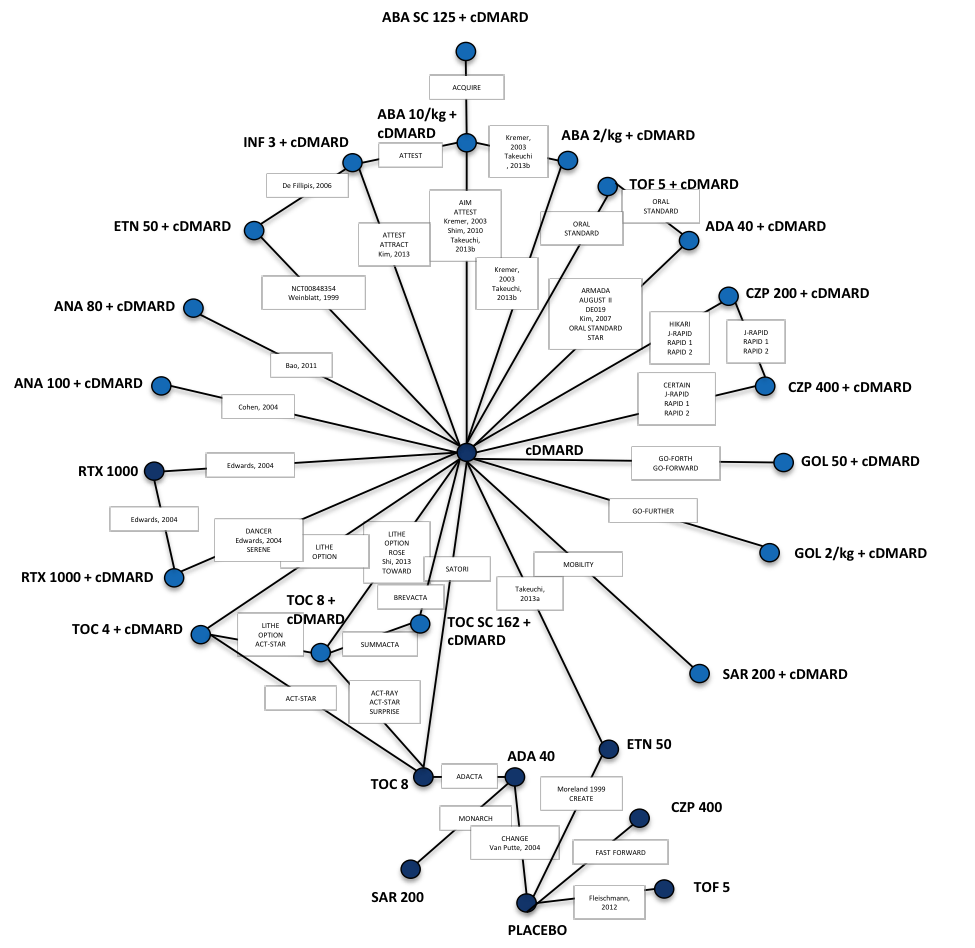
\includegraphics{evidence-network.png}
\vspace*{10mm}
\caption{Evidence network, tDMARD naive population}\label{fig:evidence-network}
\end{figure}

\subsubsection{Study specific 6-month data, tDMARD naive population}

\begin{center}
\scriptsize
\renewcommand*{\arraystretch}{1}
\begin{longtable}{@{\extracolsep{\fill}}lp{.1\linewidth}rcrrrrr}
\caption{Study specific data} \label{tbl:trial-data} \\
\hline
  \multicolumn{1}{l}{} & 
  \multicolumn{1}{c}{} & 
  \multicolumn{1}{c}{ACR 20} & 
  \multicolumn{1}{c}{ACR 50} & 
  \multicolumn{1}{c}{ACR 70} & 
  \multicolumn{1}{c}{$\Delta$DAS28} & 
  \multicolumn{1}{c}{$\Delta$HAQ-DI} \\

  \multicolumn{1}{l}{Trial ID} & 
  \multicolumn{1}{c}{Treatment} & 
  \multicolumn{1}{c}{(\%)} & 
  \multicolumn{1}{c}{(\%)} & 
  \multicolumn{1}{c}{(\%)} & 
  \multicolumn{1}{c}{(SE)} & 
  \multicolumn{1}{c}{(SE)} \\
  \hline 
  
\endfirsthead
  \caption[]{Study specific data}\\
  \hline
  \multicolumn{1}{l}{} & 
  \multicolumn{1}{c}{} &  
  \multicolumn{1}{c}{ACR 20} & 
  \multicolumn{1}{c}{ACR 50} & 
  \multicolumn{1}{c}{ACR 70} & 
  \multicolumn{1}{c}{$\Delta$DAS28} & 
  \multicolumn{1}{c}{$\Delta$HAQ} \\

  \multicolumn{1}{l}{Trial ID} & 
  \multicolumn{1}{c}{Treatment} &  
  \multicolumn{1}{c}{(\%)} & 
  \multicolumn{1}{c}{(\%)} & 
  \multicolumn{1}{c}{(\%)} & 
  \multicolumn{1}{c}{(SE)} & 
  \multicolumn{1}{c}{(SE)} \\
  \hline
\endhead
\hline
\multicolumn{2}{l}{Continued on next page}\\
\endfoot
\multicolumn{9}{l}{Note: $\Delta$DAS28 and $\Delta$HAQ denote differences between the end of the trial and baseline.}\\
\endlastfoot
\ExpandableInput{tables/trial-data.txt}
\hline
\end{longtable}
\end{center}


\subsection{Comparing the IVI NMA to the NICE NMA}\label{app:nma-ivi-nice-comp}
To help ensure that differences in cost-effectiveness estimates from our model relative to others are not driven by the NMA results, we compared our NMA estimates to estimates reported by NICE in \citet{stevenson2016adalimumab}. We focus on ACR response, since the NICE report and other models use treatment pathways similar to \textbf{H1} and \textbf{H2} and rarely use DAS28 to inform treatment duration. As shown in \autoref{tbl:nma-acr-nice-vs-ivi}, our results are similar and the NICE point estimates are generally within the 95\% credible intervals surrounding our point estimates.

\begin{table}[!ht]
\begin{center}
\scriptsize
\begin{threeparttable}
\caption{A comparison of NICE and IVI estimates of ACR response probabilities} \label{tbl:nma-acr-nice-vs-ivi}
\begin{tabularx}{\textwidth}{@{\extracolsep{\fill}}lrrrrrr}
\hline
\multicolumn{1}{c}{} & \multicolumn{3}{c}{IVI} & \multicolumn{3}{c}{NICE}\\
\cmidrule(lr){2-4} \cmidrule(lr){5-7}
\multicolumn{1}{l}{} & \multicolumn{1}{c}{ACR20} & \multicolumn{1}{c}{ACR50} & \multicolumn{1}{c}{ACR70} & \multicolumn{1}{c}{ACR20} & \multicolumn{1}{c}{ACR50} & \multicolumn{1}{c}{ACR70}\\
\hline
\ExpandableInput{tables/nma-acr-nice-vs-ivi.txt}
\hline
\end{tabularx}
\scriptsize
Notes: ACR20/50/70 categories are the probability of at least a 20/50/70\% improvement. 95\% credible intervals are in parentheses. IVI estimates are based on 6-month simulations of 1,000 patients and 1,000 parameters sets for each therapy. NICE estimates are from Table 37 in \citet{stevenson2017cost}. cDMARDs = conventional disease-modifying antirheumatic drugs; MTX = methotrexate; ABT IV = abatacept intravenous; ADA = adalimumab; ETN = etanercept; GOL = golimumab; IFX = infliximab; TCZ = tocilizumab; CZP = certolizumab pegol; ABT SC = abatacept subcutaneous; RTX = rituximab; TOF = tofacitinib. ACR = American College of Rheumatology.
\end{threeparttable}
\end{center}
\end{table}

\end{appendices}

\pdfbookmark[1]{References}{References}
\bibliography{../../vignettes/vignettes}

\end{document}
